\documentclass[fr]{../../../eplsummary}

\usepackage{../../../eplunits}
\usepackage{../../../eplelec}
\usepackage{circuitikz}
\sisetup{detect-all}
\usepackage[makeroom]{cancel}
\usepackage{amsmath,mathtools}
\usepackage{multicol}
\usepackage{float}
\usepackage{trimclip}
\usepackage{soul}

\newcommand{\Ueff}{U_\text{eff}}
\newcommand{\Ieff}{I_\text{eff}}
\newcommand{\Umr}{U_\text{moy,r}}
\newcommand{\Imr}{I_\text{moy,r}}
\newcommand{\Up}{\bar{U}}
\newcommand{\Ip}{\bar{I}}
\newcommand{\Zp}{\bar{Z}}
\newcommand{\Icc}{I_\text{cc}}
\newcommand\numberthis{\addtocounter{equation}{1}\tag{\theequation}}
\newcommand\encircle[1]{%
  \tikz[baseline=(X.base)] 
    \node (X) [draw, shape=circle, inner sep=0] {\strut #1};}
\def\doubleunderline#1{\underline{\underline{#1}}}
\def\Perp{\perp\!\!\!\perp}
\def\utilde#1{\mathord{\vtop{\ialign{##\crcr
$\hfil\displaystyle{#1}\hfil$\crcr\noalign{\kern1.5pt\nointerlineskip}
$\hfil\tilde{}\hfil$\crcr\noalign{\kern1.5pt}}}}}

\makeatletter
\providecommand\add@text{}
\renewcommand\u[1]{%
  \gdef\add@text{[\si{#1}\gdef\add@text{}]}}% 
\renewcommand\tagform@[1]{%
  \maketag@@@{\llap{\add@text\quad}(\ignorespaces#1\unskip\@@italiccorr)}%
}
\newenvironment{Figure}
  {\par\medskip\noindent\minipage{\linewidth}}
  {\endminipage\par\medskip}

\usepackage{tikz}
\usetikzlibrary{arrows,shapes,positioning,shadows,trees}


\tikzset{
  basic/.style  = {draw, text width=6cm, drop shadow, font=\sffamily, rectangle},
  root/.style   = {basic, rounded corners=2pt, thin, align=center,
                   fill=green!30},
  level 2/.style = {basic, rounded corners=6pt, thin,align=center, fill=green!60,
                   text width=12em},
  level 3/.style = {basic, thin, align=left, fill=pink!60, text width=8em}
}
\def\Perp{\perp\!\!\!\perp}

\hypertitle{Télécommunications}{6}{ELEC}{1360}
{Louis Colin}
{Luc Vandendorpe}



\part{Introduction}

\section{Les sources d'information}

Les plus communément rencontrées sont \textit{la parole}, \textit{la musique},\textit{les images ou la vidéo} et \textit{les données d'ordinateur}. Dans le cadre de la parole, de la musique ou encore des données numériques, le signal est monodimensionnel. Les images sont transmises via un signal bidimensionnel  $(x,y)$ les coordonnées horizontales et verticales et la vidéo n'est qu'une suite d'images dans le temps ce qui en fait un signal tridimensionnel $(x,y,t)$.\\
Le signal peut aussi être vectoriel ou scalaire. Le son par exemple est scalaire (sauf dans le cas du stéréo) et la vidéo en couleur nécessitera une transmission d'un vecteur de trois signaux bidimensionnels.

\subsection{La parole et la musique}

Le son se propage dans l'air sous forme d'onde de pression à 300 m/s. Son intensité décroît donc avec le cube de la distance à la source ponctuelle et est donnée en $\left[ \frac{W}{cm^2} \right]$, au même pied que le vecteur de Poynting en électricité.\\
L'oreille humaine est sensible au logarithme d'un rapport d'intensité. On ressentira la même sensation d'accroissement entre une intensité de 10 et 100 qu'entre une intensité de 20-200. C'est pourquoi on mesurera l'intensité acoustique en $dB_{ac}$ comme :
$$ I_{dB_{ac}} = 10\ \log_{10} [I/(10^{-16}\ W/cm^2)] $$
La valeur de $10^{-16}\ W/cm^2$ représente le seuil d'audibilité de la fréquence de $1 kHz$ qui est la fréquence de sensibilité maximale.\\

En raison des effets de résonance du canal auditif et de la fonction de transfert des organes présents dans l'oreille interne, l'oreille n'est pas identiquement sensible à toutes les fréquences. Le diagramme de Fletcher-Munson nous montre que la dynamique de l'oreille est de l'ordre de 120 dB. 

\begin{figure}[H]
    \centering
    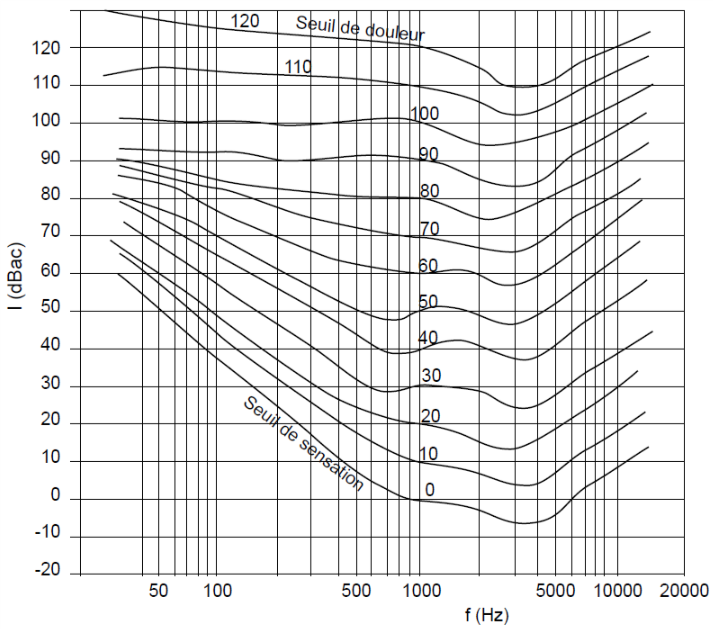
\includegraphics[width=0.5\textwidth]{img/fletcher.png}
    \caption{diagramme de Fletcher-Munson}
\end{figure}

Les niveaux subjectifs sont exprimés pour des sons purs
\footnote{Pour les sons non sinusoïdaux l’on recourt à
la notion de volume qui est une intensité pondérée par la sensibilité de l’oreille en fonction de la fréquence et est exprimée en sones.}
 en \textit{phones}. Il s'agit de l'intensité objective qui, à 1 kHz produirait la même sensation de niveau sonore. On remarque que 40$dB_{ac}$ à 200 Hz correspond à 20 phones. \\
On notera les différents niveaux de bruit ambiant :
\begin{itemize}
\item
calme complet : 40 $dB_{ac}$
\item
conversation normale : 70 $dB_{ac}$
\item
niveau permanent max permis par le règlement général sur la protection du travail : 90 $dB_{ac}$
\item
train sur le quai : 110 $dB_{ac}$
\item
sono dans une soirée : 120 $dB_{ac}$
\end{itemize}

L'oreille est aussi sensible à la fréquence des sons, là encore de manière logarithmique. Une \textit{décade} exprime un rapport de fréquences de 10 et une  \textit{octave}, un rapport de 2. Le seuil de sensibilité en fréquence est de l'ordre d'un \textit{comma} $\simeq 1/45$ \textit{octave}.\\

Le diagramme de Fletcher-Munson montre qu'une oreille en bon état entend des fréquences entre \textbf{50} et \textbf{16000} Hz environ. Cependant, on ne retransmet pas l'intégralité de cette bande de fréquences à l'émission. En radio AM, on ne reproduit les fréquences que jusque \textbf{4500}Hz pour une qualité raisonnable. En \textit{téléphonie}, où l'objectif est l'intelligibilité du message, la bande de fréquences normalisée est de \textbf{300 à 3400} Hz.

\subsection{Image et vidéo}

\subsubsection*{monochrome ou noir et blanc}

Les images en mouvement de type \textit{monochrome} sont transmises via le signal de \textit{luminance} qui est une information dépendant du temps, et des deux coordonnées spatiales $Y(x,y,t) \in \mathbb{R^+}$. Si l'on veut transmettre cette information qui ne dépende que du temps, il faut nécessairement passer par deux étapes d'échantillonnage. La première se fait selon le temps, à savoir ne capturer l'information qu'au droit d'un nombre fini de positions temporelles. Pour cela, il est nécessaire de dépasser la capacité d'absorption du cerveau qui va saturer au delà de 10 à 20 fps. Deux problèmes vont alors se poser :\\
Avec de telles cadences, l’œil humain perçoit un phénomène de papillotement. De plus, certains parasites sur le réseau électrique peuvent venir se superposer au signal et ainsi produire un défilement sur l'image si les deux fréquences sont différentes.\\
En vue de convertir notre signal bidimensionnel en un signal monodimensionnel, on procède au second échantillonnage dans la dimension verticale cette fois-ci. L'image sera donc divisée en lignes horizontales, dont le nombre minimum peut-être déterminé en fonction du pouvoir de résolution de l’œil qui est de l'ordre de la minute d'arc soit $\frac{1}{60}^{\circ}$. Un observateur situé à une distance de six fois la hauteur de l'écran ne pourra distinguer plus de 500 lignes sur l'écran.\\
Pour venir à bout de l'effet de papillotement, on aura recours à \textit{l'entrelacement}. Cette technique consiste à diviser chaque image en deux sous-ensembles appelés \textit{trames}. La première trame contient les lignes paires et la seconde les lignes impaires. On présentera les deux trames 25 fois par seconde ce qui nous écarte du problème de papillotement. La fréquence de trame est donc de 50 Hz qui est choisie pour coller à la fréquence de réseau pour annuler l'effet de défilement. La fréquence de réseau a donc un impact sur le nombre d'images par seconde (fps). On aura les paramètres suivants pour les deux systèmes de télévision mondiaux principaux :

\begin{table}[H]
\centering
\begin{tabular}{|l|l|l|}
\hline
 \textbf{Paramètres}&\textbf{Syst. B,G,I}  &\textbf{Syst. M}  \\ \hline
Fréquence d'image & 25 Hz  & 30 Hz (env.) \\ 
Nombre de lignes & 625 & 525 \\ 
Fréquence de ligne & 15 625 Hz & 15 750 Hz (env.) \\ 
Durée de ligne & 64 $\mu s$ & 63.5 $\mu s$ \\ 
Durée active de la ligne & 51.7 - 52.2 $\mu s$ & 52.1-53.3 $\mu s$ \\ 
Suppression de ligne & 11.8 - 12.3 $\mu s$  & 10.2 - 11.4 $\mu s$  \\ 
Impulsion synchro & 4.5 - 4.9 $\mu s$  & 4.19 - 5.7 $\mu s$  \\ 
Durée de trame & 20 ms & 16.667 ms (env.) \\ 
Suppression de trame & 1.612 ms & 1.217-1.344 ms \\ 
 & (25 lignes) & (19-21 lignes) \\ 
Partie active de la trame & 18.388 ms & 15.323-15.450 ms \\ 
Nombre de lignes actives & 575 & 485 \\ \hline
\end{tabular}
\caption{Paramètres des systèmes de télévision}
\end{table}

La figure \ref{lum} représente le signal de luminance correspondant à une ligne de télévision monochrome, il varie de 0 à 1 Volt. La partie comprise entre 0,3V et 1V détermine la luminosité du spot : en fait, quand le signal est inférieur à 0,375V le spot est noir (éteint) ; quand il est à 1Volt, le spot est blanc (luminosité maximale) entre 0,375 et 1 V il est gris plus ou moins foncé suivant la tension.

\begin{figure}[H]
    \centering
    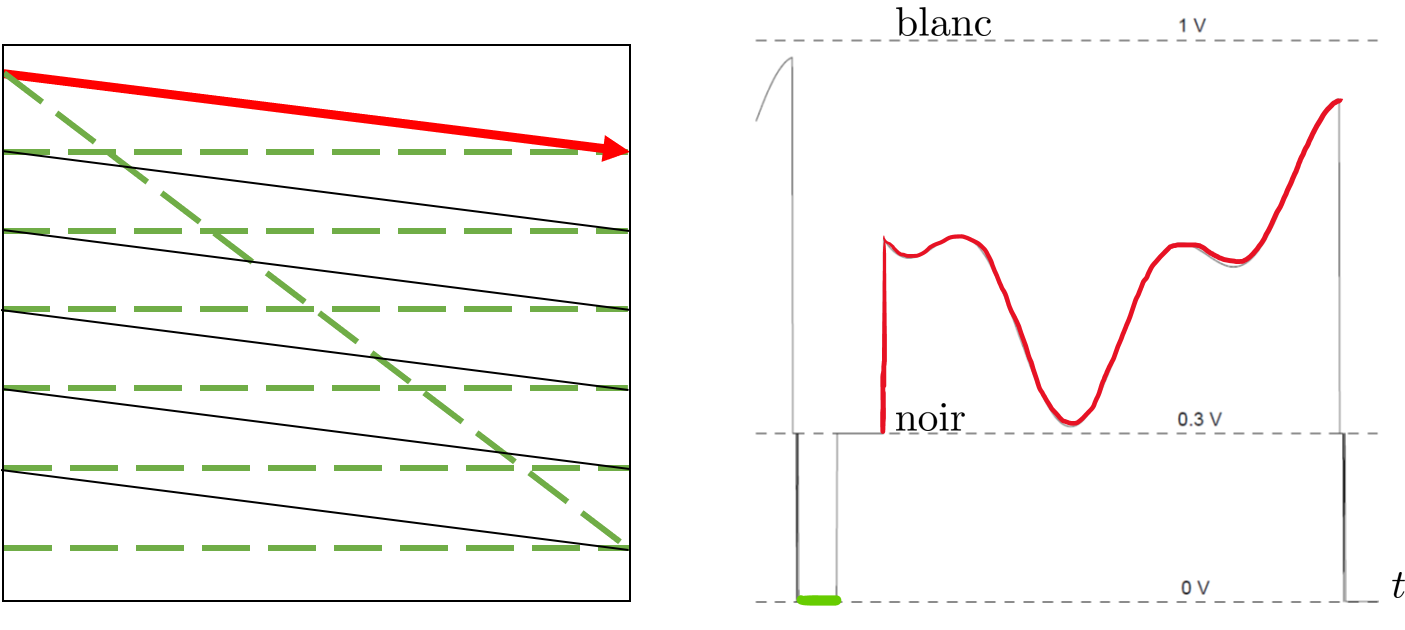
\includegraphics[width=0.75\textwidth]{img/luminance.png}
    \caption{Signal de luminance sur une ligne}
    \label{lum}
\end{figure}

La bande passante requise sera déterminée par la vitesse de variation de la luminance sur les lignes. On déterminera la fréquence maximale en exigeant que les résolutions horizontales et verticales soient les mêmes. Si on a un rapport de Largeur/Hauteur de 4/3 avec $N_l$ lignes, cela équivaut à $4N_l/3$ points (échantillons) par ligne. En vertu du théorème de Shannon, la résolution sera la demi-fréquence d'échantillonnage soit $2N_l/3$ cycles par ligne. La fréquence de ligne étant $f_l$, on aura $2N_lf_l/3$ cycles/sec $= 2\times 575\times 15625/3 = 5.98 MHz $. On retiendra que le spectre s'étend jusque \textbf{5 à 6} MHz. 

\begin{figure}[H]
    \centering
    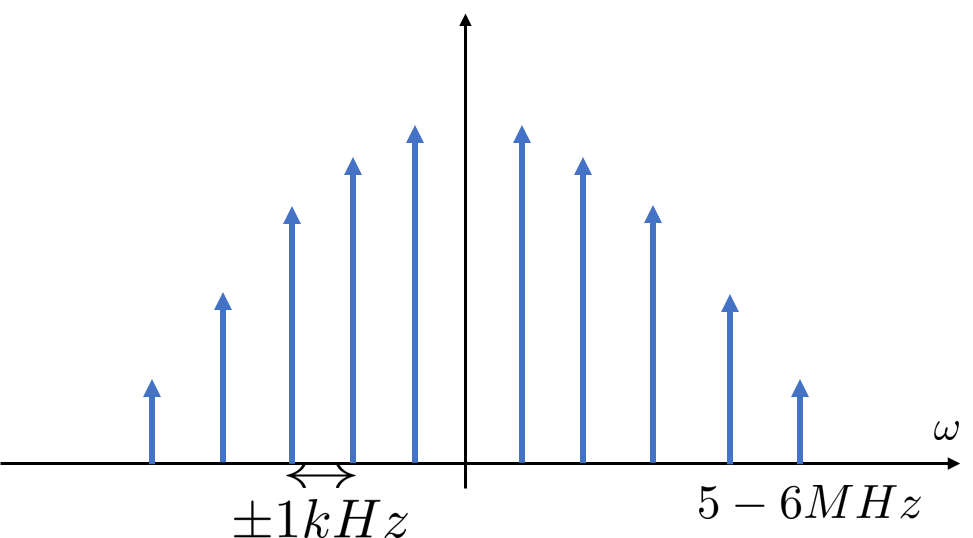
\includegraphics[width=0.3\textwidth]{img/lumF.png}
    \caption{Signal de luminance dans le domaine fréquentiel}
    \label{lumF}
\end{figure}


\subsubsection{La couleur}

On peut reconstituer une teinte et une luminance arbitraires à partir de trois \textit{couleurs primaires} quelconques. On peut donc représenter une lumière quelconque par un vecteur dans l'espace dont les vecteurs de base correspondent aux trois primaires choisies. On peut passer d'un triplet de primaires à un autre par une opération de produit matriciel (changement de base). Le choix des primaires utilisées pour la transmission a été guidé par les considérations suivantes :
\begin{itemize}
\item
l'une des primaires doit être la luminance de manière à permettre à un récepteur monochrome de pouvoir décoder un signal émis en couleur. 
\item
les deux autres primaires contenant l'information de couleur, doivent être telles que leur bande passante soit aussi petite que possible statistiquement sur un grand nombre d'images. Elles doivent en fait venir s'intercaler entre les raies du signal de luminance voir \ref{lumF}
\end{itemize}
Il existe ainsi un système de trois vecteurs orthogonaux $(\vec{x},\vec{y},\vec{z})$ défini par la commission internationale de l'éclairage dont on retiendra que la coordonnée le long de $\vec{y}$ représente bien la luminance et que toutes les lumières réelles ont des coordonnées positives dans ce système.\\
On représente les \textit{couleurs} par les coordonnées de \textit{chromaticité} définies par :
\begin{align*}
x &= \frac{X}{X+Y+Z} \\
y &= \frac{Y}{X+Y+Z} \\
z &= \frac{Z}{X+Y+Z} = 1-x-y
\end{align*}
Ces coordonnées sont donc débarrassées du facteur d'amplitude correspondant à la luminance. De plus, deux d'entre elles définissent la troisième. On peut donc recourir à une représentation dans un plan appelé \textit{diagramme de chromaticité} ou \textit{triangle des couleurs}.

\begin{figure}[H]
    \centering
    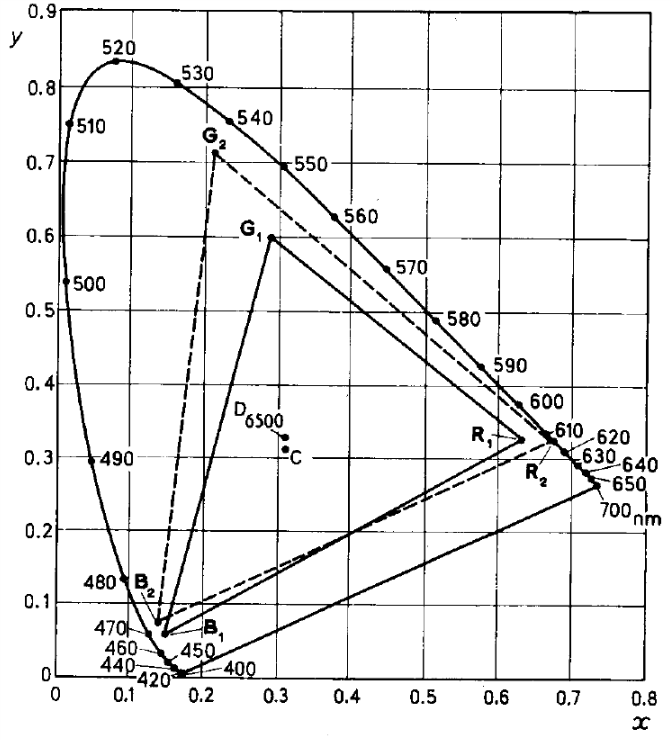
\includegraphics[width=0.5\textwidth]{img/Triangle.png}
    \caption{Triangle des couleurs}
\end{figure}

\section{Canaux de communication}

Le canal de communication est le véritable support au signal envoyé. On peut les classer en deux grandes familles : ceux où la propagation est \textit{guidée} et ceux où elle est \textit{libre}.\\
La première famille comprend les lignes téléphoniques, les câbles coaxiaux et les fibres optiques. On regroupe aussi les lignes et les câbles sous une même appellation de \textit{lignes métalliques}, constituée de deux conducteurs l'un aller et l'autre retour. Une telle ligne comporte des paramètres importants fonctions de la fréquence tels que la résistance linéique $R\ [\Omega/m]$, inductance linéique $L\ [H/m]$, la capacitance linéique $C\ [F/m]$ ou la perditance linéique $G\ [S/m]$.\\
La seconde famille de canaux comprend les canaux de radiodiffusion, les canaux pour mobiles et les canaux pour satellites.

\subsection{Les paires torsadées}

Les câbles téléphoniques contiennent de nombreuses paires de conducteurs. Si les fils sont agencés de manière parallèle, le couplage entre circuits peut être très élevé et provoquer de la diaphonie. On peut réduire ces interférences en torsadant les paires avec un pas bien défini. 

\subsection{Câbles coaxiaux}

Un câble coaxial est constitué d’une partie centrale (fil de cuivre) enveloppé dans un isolant, puis d’un blindage métallique tressé et enfin d’une gaine extérieure. Il est utilisé comme câble pour la transmission de la télédistribution. Il profite d'une large bande passante et d'une meilleur protection contre les interférences qu'un câble classique. 

\subsection{Fibre optique}

Une fibre optique est un conducteur de lumière en fil en verre ou en plastique très fin utilisé pour la transmission de données (sous forme de lumière). Un mode est un chemin emprunté par la lumière par rapport à sa réflexion et réfraction au sein de la fibre optique. Les plus gros avantages de la fibre optique est qu'elle bénéficie d'une énorme bande passante. Les ondes peuvent néanmoins interagir avec les structures moléculaires du verre et les impuretés mais les atténuations restent très faibles.

\subsection{Ondes radio}

\begin{figure}[H]
    \centering
    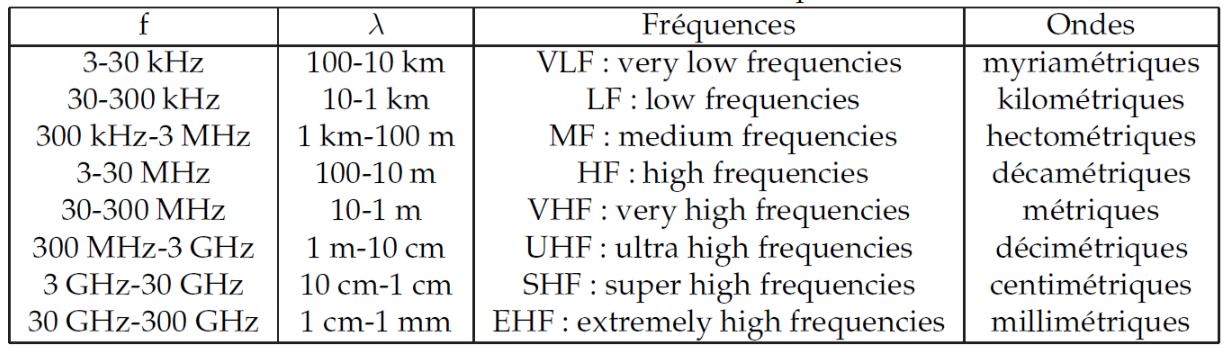
\includegraphics[width=0.8\textwidth]{img/ondesradio.png}
    \caption{caractéristiques des différentes bandes de fréquences avec leur nom}
\end{figure}

\begin{figure}[H]
\tiny
\centering
\begin{picture}(500,162)
	%\put(0,0){\framebox(500,180)}
	% Longueur d'onde
	\put(500,152){\vector(-1,0){430}}
	\put(100,150){\line(0,1){4}} \put(90,156){1Mm}
	\put(130,150){\line(0,1){4}} \put(120,156){100km}
	\put(160,150){\line(0,1){4}} \put(153,156){10km}
	\put(190,150){\line(0,1){4}} \put(184,156){1km}
	\put(220,150){\line(0,1){4}} \put(212,156){100m}
	\put(250,150){\line(0,1){4}} \put(243,156){10m}
	\put(280,150){\line(0,1){4}} \put(275,156){1m}
	\put(310,150){\line(0,1){4}} \put(302,156){10cm}
	\put(340,150){\line(0,1){4}} \put(334,156){1cm}
	\put(370,150){\line(0,1){4}} \put(362,156){1mm}
	\put(400,150){\line(0,1){4}} \put(391,156){100$\mu$m}
	\put(430,150){\line(0,1){4}} \put(423,156){10$\mu$m}
	\put(460,150){\line(0,1){4}} \put(453,156){1$\mu$m}
	\put(0,150){Longueur d'onde}
	\put(60,150){$\lambda$}
	% Fréquence
	\put(0,130){Fréquence}
	\put(70,132){\vector(1,0){430}}
	\put(85,130){\line(0,1){4}} \put(77,122){100Hz}
	\put(115,130){\line(0,1){4}} \put(107,122){1kHz}
	\put(145,130){\line(0,1){4}} \put(134,122){10kHz}
	\put(175,130){\line(0,1){4}} \put(165,122){100kHz}
	\put(205,130){\line(0,1){4}} \put(195,122){1MHz}
	\put(235,130){\line(0,1){4}} \put(222,122){10MHz}
	\put(265,130){\line(0,1){4}} \put(251,122){100MHz}
	\put(295,130){\line(0,1){4}} \put(286,122){1GHz}
	\put(325,130){\line(0,1){4}} \put(314,122){10GHz}
	\put(355,130){\line(0,1){4}} \put(342,122){100GHz}
	\put(385,130){\line(0,1){4}} \put(376,122){1THz}
	\put(415,130){\line(0,1){4}} \put(404,122){10THz}
	\put(445,130){\line(0,1){4}} \put(432,122){100THz}
	\put(475,130){\line(0,1){4}} \put(466,122){1PHz}
	% Pointille
	\multiput(85,120)(0,-4){30}{\line(0,-1){2}}
	\multiput(115,120)(0,-4){30}{\line(0,-1){2}}
	\multiput(145,120)(0,-4){5}{\line(0,-1){2}}
	\multiput(175,120)(0,-4){5}{\line(0,-1){2}}
	\multiput(205,120)(0,-4){5}{\line(0,-1){2}}
	\multiput(235,120)(0,-4){5}{\line(0,-1){2}}
	\multiput(265,120)(0,-4){5}{\line(0,-1){2}}
	\multiput(295,120)(0,-4){5}{\line(0,-1){2}}
	\multiput(325,120)(0,-4){5}{\line(0,-1){2}}
	\multiput(355,120)(0,-4){5}{\line(0,-1){2}}
	\multiput(385,120)(0,-4){22}{\line(0,-1){2}}
	\multiput(385,16)(0,-4){4}{\line(0,-1){2}}
	\multiput(415,120)(0,-4){30}{\line(0,-1){2}}
	\multiput(445,120)(0,-4){30}{\line(0,-1){2}}
	\multiput(475,120)(0,-4){30}{\line(0,-1){2}}
	\put(130,82){\framebox(30,18){VLF}}
	\put(160,82){\framebox(30,18){LF}}\put(170,74){km}
	\put(190,82){\framebox(30,18){MF}}\put(200,74){hm}
	\put(220,82){\framebox(30,18){HF}}\put(228,74){dam}
	\put(250,82){\framebox(30,18){VHF}}\put(262,74){m}
	\put(280,82){\framebox(30,18){UHF}}\put(290,74){dm}
	\put(310,82){\framebox(30,18){SHF}}\put(320,74){cm}
	\put(340,82){\framebox(30,18){EHF}}\put(350,74){mm}
	\put(0,92){Désignation}
	\put(0,84){internationale}
	% Pointille sous boite
	\multiput(145,80)(0,-4){20}{\line(0,-1){2}}
	\multiput(175,72)(0,-4){18}{\line(0,-1){2}}
	\multiput(205,72)(0,-4){18}{\line(0,-1){2}}
	\multiput(235,72)(0,-4){18}{\line(0,-1){2}}
	\multiput(265,72)(0,-4){2}{\line(0,-1){2}}
	\multiput(265,56)(0,-4){14}{\line(0,-1){2}}
	\multiput(295,72)(0,-4){5}{\line(0,-1){2}}
	\multiput(295,44)(0,-4){11}{\line(0,-1){2}}
	\multiput(325,72)(0,-4){5}{\line(0,-1){2}}
	\multiput(325,36)(0,-4){9}{\line(0,-1){2}}
	\multiput(355,72)(0,-4){7}{\line(0,-1){2}}
	\multiput(355,24)(0,-4){6}{\line(0,-1){2}}
	% Line
  \textcolor{red}{\put(145,60){\line(1,0){90}}} \put(240,58){onde de sol}
  \textcolor{blue}{\put(175,50){\line(1,0){90}} }\put(270,48){réflection ionosphérique}
  \textcolor{orange}{\put(235,40){\line(1,0){60}}} \put(300,38){réfraction troposphérique}
  \textcolor{purple}{\put(265,30){\line(1,0){60}} }\put(330,28){dispersion troposphérique}
  \textcolor{green}{\put(235,20){\line(1,0){120}}} \put(360,18){visibilité directe}
\end{picture}
\normalsize
\caption{Les différentes techniques de propagation}
\end{figure}


Il existe plusieurs modes de propagation :
\begin{itemize}
\item
par onde directe :\\

Les ondes directes sont envoyées en ligne droite d’une antenne à une autre. Elles ont une portée relativement limitée et il y a des interférences avec l’onde réfléchie sur la terre. \textit{(En effet entre deux antennes il existe deux chemins : l’un direct et l’autre avec une réflexion de l’onde sur la terre).}
\item
par onde de sol :\\

Les ondes de sol utilisent des ondes basse fréquence qui ont tendance à
se propager le long du sol,\textit{ selon une propriété de celle ci}. En
effet, les fronts d'ondes des ondes basses fréquences se déplacent perpendiculairement au sol.
\begin{figure}[H]
\centering
\begin{tabular}{ll}
\hline
Frequence & Portée (km)\\
\hline
$100 kHz$ & $200$\\
$1 MHz$ & $60$\\
$10 MHz$ & $6$\\
$100 MHz$ & $1.5$\\
\hline
\end{tabular}
\end{figure}

\item
par réflexion/réfraction sur l'ionosphère :\\

Sous l'effet de l'\textbf{ionisation} de l'air par les UV solaires, la
densité en électrons des couches de l'ionosphère les plus éloignées
augmentent. Ainsi ce \og{}mur\fg{} d'électrons cause la réfraction,
voire même la réflexion des signaux. On reconnait \textbf{4 couches
précises} (càd 4 endroits où la densité augmente de facon
particulièrement rapide). De la plus proche à la plus éloignée de la
Terre, la couche $D$, $E$, $F_1$ et $F_2$ (ces deux dernières devenant une seule pendant la nuit, la couche $F$).

Grâce à cette propagation, on peut faire \og{}rebondir\fg{} des ondes
sur ces couches et propager une onde entre les continents (au-delà de
l'horizon). On utilise massivement cette technique pour les ondes de hautes fréquence.

\item
par satellite :\\

Pour transmettre ces signaux, on envoie des ondes directement d'une antenne à un satellite géostationnaire se trouvant sur une orbite équatoriale à $36.000km$ d'altitude. Ensuite le satellite renvoi le signal vers une antenne au sol.

\end{itemize}





\part{Fonction aléatoires}

\begin{itemize} 
\renewcommand{\labelitemi}{$\bullet$}
\renewcommand{\labelitemii}{$\cdot$}
\setlength\itemsep{1em}

\item Un \textcolor{red}{\textbf{R}andom \textbf{Signal}} est une \textcolor{red}{\textbf{R}andom \textbf{V}ariable} pour chaque valeur de la variable indépendante (ex: $t$)\\
ex: pour un $t_1$, $X(t_1)$ est une RV avec pour \textcolor{red}{pdf} : $T_X[x(t_1)]$ et \textcolor{red}{cdf} : $F_X[x(t_1)]$

\item \textcolor{red}{Moyenne} : $m_X(t) = \textbf{E}[X(t)] = \int_{-\infty}^{\infty} xT_X[x(t)]dx$

\item \textcolor{red}{Variance} : $\sigma_X^2(t) = \textbf{E}[X_c(t)\ X_c^*(t)]$

\item \textcolor{red}{Covariance} :  $C_X(t_1,t_2) = \Gamma_X(t_1,t_2) = \textbf{E}[X_c(t_1)\ X_c^*(t_2)]\vspace{0.3cm}\\
 = \int_{x_1} \int_{x_2} [x_1-m_X(t_1)][x_2 - m_X(t_2)]^*\ T_X[x(t_1),x(t_2)]dx_1\ dx_2
\vspace{0.3cm}$

\begin{itemize}
\setlength\itemsep{0.75em}
\item $\sigma^2_X=C_X(t,t)$
\item pour des fonctions réelles : $C_X(t_1,t_2) = C_X(t_2,t_1)$
\item pour des fonctions complexes : $C_X(t_1,t_2) = C_X^*(t_2,t_1)$
\item un RS a des valeurs \textbf{décorrellées} si $C_X(t_1,t_2) = \sigma_X^2 \ \delta(t_1-t_2)$
\end{itemize}

\item \textcolor{red}{Mutual Covariance} :  $C_{XY}(t_1,t_2) = \textbf{E}[X_c(t_1)\ Y_c^*(t_2)]
\vspace{0.3cm}\\
 = \int_{x} \int_{y} [x-m_X(t_1)][y - m_Y(t_2)]^*\ T_{XY}[x(t_1),y(t_2)]dx\ dy
\vspace{0.3cm}$

\item \textcolor{red}{Matrice de covariance} : 
Soit $\begin{pmatrix}X_1 & X_2 \end{pmatrix}^T$ on aura $\utilde{C}_{\textbf{XX}} = \textbf{E}[\vec{X}_c\ \vec{X}_c^T] = \begin{pmatrix} \sigma_1^2 & C_{12} \\C_{21} & \sigma_2^2 \end{pmatrix} $

\item \textcolor{red}{VA $\mathbb{C}$} :
$Z = X+j\ Y \ \rightarrow \ T_{XY}(x,y)$

\begin{itemize}
\setlength\itemsep{0.75em}
\item 
$\sigma_Z^2 = \underbrace{\textbf{E}(Z_c\ Z_c^*)}_{\in \mathbb{R}} = \textbf{E}(|Z_c^2|) = \textbf{E}(X_c^2) + \textbf{E}(Y_c^2) = \sigma_X^2 + \sigma_Y^2$

\item $C_{Z_{1c}Z_{2c}} = \underbrace{\textbf{E}(Z_{1c}Z_{2c}^*)}_{\in \mathbb{C}}$

\item $\vec{Z} = \begin{pmatrix}Z_1 & Z_2 \end{pmatrix}^T \rightarrow \utilde{C}_{\textbf{ZZ}} = \textbf{E}(\vec{Z}_c \ \vec{Z}_c^{T,*})$
\end{itemize}

\item \textcolor{red}{Stationnarité au sens stricte (SSS)}: les PDFs de n'importe quel ordre ne dépendent pas des origines des axes. Dépend seulement de \textbf{$\neq$ de temps}.
\vspace{-2ex}
\begin{align*}
T_X[x(t)] &= T_X(x) \\
T_X[x(t_1),x(t_2),...,x(t_n)] &= T_X[x(0),x(t_2-t_1),...,x(t_n-t_1)]
\end{align*}

\item \textcolor{red}{Stationnarité au sens faible (WSS)}: Idem mais limité à l'ordre 2:
\vspace{-2ex}
\begin{align*}
T_X[x(t)] &= T_X(x) \\
T_X[x(t_1),x(t_2)] &= T_X[x(0),x(t_2-t_1)]
\end{align*}

\begin{itemize}
\item \textcolor{blue}{Propriétés} :
\begin{align*}
\text{Moyenne constante}&: \\
m_X(t) &\stackrel{\textcolor{blue}{(1A)}}{=} m_X \\
\text{Covariance dépendante de } \tau &: \\
C_X(t_1,t_2) &\stackrel{\textcolor{blue}{(1B)}}{=} C_X(t_1-t_2,0) = C_X(\tau)
\end{align*}
$\rightarrow \sigma_X^2(t) = C_X(t,t) = C_X(0) = \sigma_X^2$
\end{itemize}


\item \textcolor{red}{Ergodism}: 
C'est l'étude des conditions sous lesquelles une moyenne d'ensemble peut être remplacée par une moyenne temporelle.
\begin{multicols}{2}
\noindent
ensemble averaging:
\begin{Figure}
    \centering
    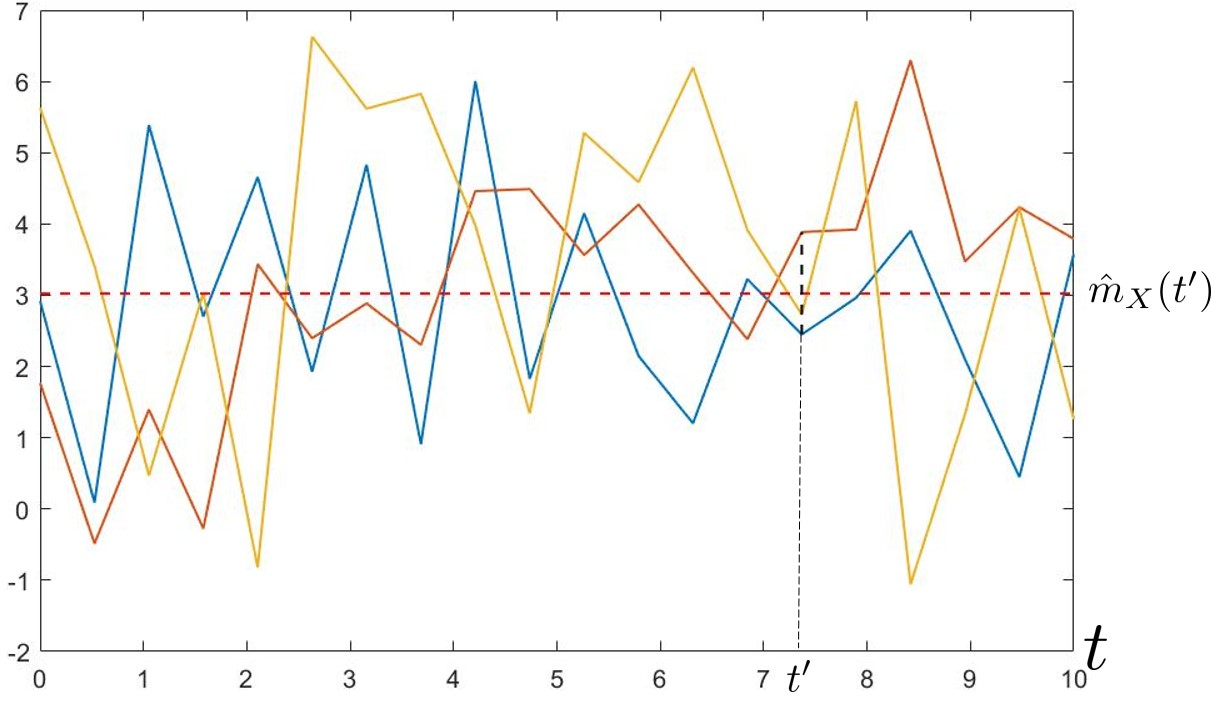
\includegraphics[width=0.9\textwidth]{img/mX.jpg}
\end{Figure}

$$\hat{m}_X(t') = \frac{1}{K} \sum_{k=1}^{K} x_k(t')$$
\vfill\null
\columnbreak
time averaging:
\noindent
\begin{Figure}
    \centering
	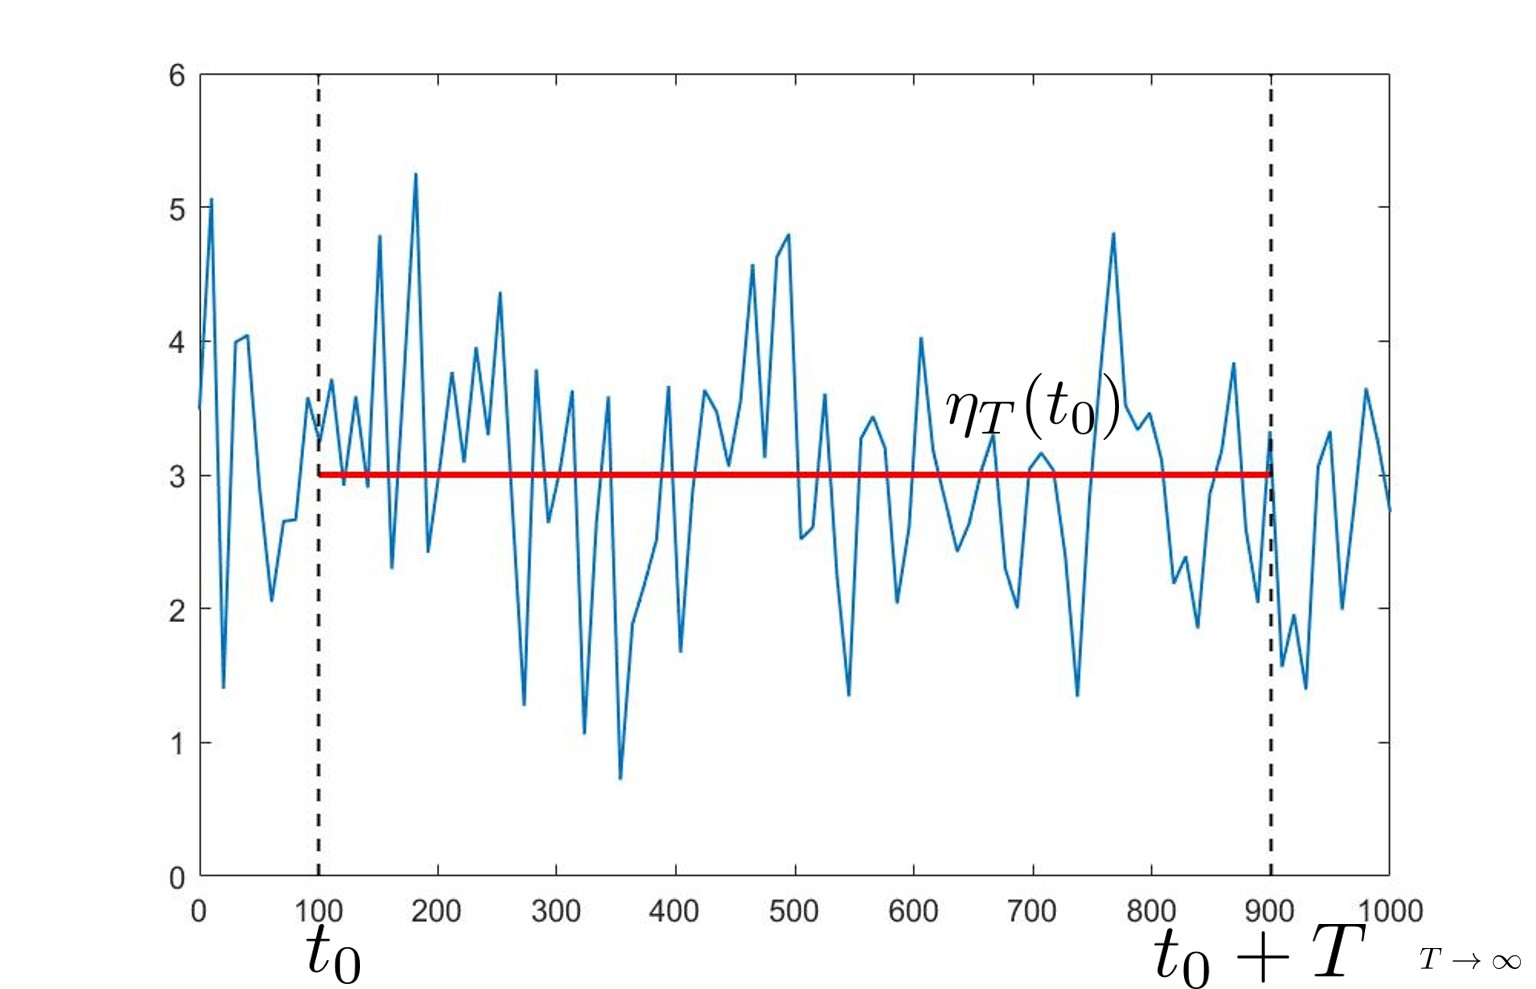
\includegraphics[width=0.9\textwidth]{img/nT.jpg}
\end{Figure}

$$ \eta_T(t_0) = \frac{1}{T} \int_{t_0}^{t_0+T} X(t)dt$$
\vfill\null
\end{multicols}

Il y a \textcolor{red}{ergodisme p/r à la moyenne} si:
$\lim_{T \to \infty} \eta_T(t_0) = m_X$

\item \textcolor{red}{Fonction de corrélation $\phi_X(\tau,t_0)$} d'un RS WSS $X(t)$ :
$$\phi_X(\tau,t_0) = \frac{1}{T} \int_{t_0}^{t_0+T} \left[ X(t+\tau) - \eta_T(t_0+\tau)\right]
\left[ X(t) - \eta_T(t_0)\right]^* dt$$
Il y a \textcolor{red}{ergodisme p/r à $\phi_X(\tau,t_0)$} si :

\begin{itemize}
\item il y a ergodisme p/r à la moyenne ($\eta_T(t_0) \rightarrow m_X$)
\item $\lim_{T \to \infty} \phi_T(\tau,t_0) = C_X(\tau)$
\end{itemize}

%\begin{itemize}
%\item
%il y a ergodisme par rapport à la moyenne ($\eta_T(t_0) \rightarrow m_X$)
%\item
% $\lim_{T \to \infty} \phi_T(\tau,t_0) = C_X(\tau)$
%\end{itemize}

$$ \textcolor{red}{\rightarrow}\ C_X(0) = \sigma_X^2 = \lim_{T \to \infty} \frac{1}{T} \int_{t_0}^{t_0+T} | \underbrace{x(t)}_{AC} - \underbrace{m_x}_{DC} | ^2 dt = \text{Puissance contenue dans le signal} $$

\underline{NB}: $\phi_X(\tau, t_0)$ est une variable non déterministe tandis que $C_{x_1,x_2}$ est déterministe ! C'est quand $T \rightarrow \infty$ que la fonction de corrélation perd son déterminisme si il y a ergodisme.

\item \textcolor{red}{Transformées de signaux aléatoires} :
\begin{align*}
\mathcal{X}(\omega) &= \int_{-\infty}^{\infty} e^{-j\omega t} X_{\textcolor{red}{c}}(t) dt \\
X_c(t) &= \frac{1}{2\pi}\int_{-\infty}^{\infty} e^{j\omega t} \mathcal{X}(\omega) d\omega \\
\end{align*}

\item \textcolor{red}{Covariance de $\mathcal{X}(\omega)$} :
\begin{align*}
C_{\mathcal{X}}(\omega,\omega') 
&= \textbf{E}[\mathcal{X}(\omega)\mathcal{X}^*(\omega')] \\
&= \int_{t=-\infty}^{\infty}\int_{t'=-\infty}^{\infty} \textbf{E}[X_c(t)\ X_c^*(t')]e^{-j\omega t}e^{j\omega' t'} dt\ dt' \\
&\downarrow \text{pour un signal WSS}\\
&= \int_{t=-\infty}^{\infty}\int_{t'=-\infty}^{\infty} C_X(\tau)e^{-j\omega t}e^{j\omega' t'} dt\ dt' \\
&= \int_{\tau=-\infty}^{\infty} C_X(\tau) e^{-j\omega \tau}\ d\tau \ \int_{t'=-\infty}^{\infty} e^{-j(\omega-\omega') t'} dt'  \\
&\stackrel{\textcolor{blue}{(2)}}{=} \gamma_X(\omega)2\pi\underbrace{\delta(\omega-\omega')}_{\textcolor{red}{\text{décorrelle}}}
\end{align*}

La transformé de Fourier est donc l'opération qui \underline{décorrelle} un RS $X(t)$ avec des valeurs \textbf{correllées} en un signal $\mathcal{X}(\omega)$, qui a des valeurs \textbf{décorrellées} ! De plus, si on peut montrer qu'un signal a une covariance de ce type, alors il sera WSS \textcolor{blue}{(2)}.

\item \textcolor{red}{Densité spectrale de puissance}:

\begin{align*}
\gamma_X(\omega) &= \int_{-\infty}^{\infty} e^{-j\omega \tau} C_X(\tau) d\tau \\
C_X(\tau) &= \frac{1}{2\pi}\int_{-\infty}^{\infty} e^{j\omega \tau}\ \gamma_X(\omega)\ d\omega \\
\sigma_X^2 &= C_X(0) \stackrel{\textcolor{blue}{ergo}}{=} P = \int_{-\infty}^{\infty} \gamma_X(2\pi f)df
\end{align*}

$\gamma_X(\omega)$ donne donc la distribution de puissance le long de l'axe $f$. On peut donc connaitre en moyenne la puissance que les signaux aléatoires consommeront.

\item \textcolor{red}{Effets sur les systèmes LTI pour WSS}:

\begin{multicols}{2}
$Y(t) = \int_\tau X(t-\tau)g(\tau) d\tau $
\vfill\null
\columnbreak
\noindent
\begin{align*}
\rightarrow  \textbf{E}[Y(t)] &= \int_\tau \textbf{E}[X(t-\tau)]g(\tau) d\tau \\
&\stackrel{WSS}{=} m_X \int_\tau g(\tau) d\tau \\
m_Y &= m_X \ G(0) \rightarrow \textcolor{blue}{(1A)}
\end{align*}
\end{multicols}

\begin{center}
$ \mathcal{X}(\omega)\ \rightarrow \ $ \fbox{ $G(\omega) $} $\ \rightarrow \ \mathcal{Y}(\omega)) $
\end{center}
\begin{align*}
C_{\mathcal{Y}}(\omega,\omega') &= \textbf{E}[\mathcal{Y}(\omega) \mathcal{Y^*}(\omega')] \\
&= G(\omega)G^*(\omega')\textbf{E}[\mathcal{X}(\omega) \mathcal{X^*}(\omega')] \\
&= G(\omega)G^*(\omega') C_{\mathcal{X}}(\omega,\omega') \\
&= |G(\omega)|^2 C_{\mathcal{X}}(\omega,\omega') \rightarrow \ \textcolor{blue}{(1B)} \\
&= |G(\omega)|^2\ 2\pi \gamma_X(\omega)\delta(\omega - \omega')\\
&\stackrel{\textcolor{blue}{WSS}}{=} 2\pi \gamma_Y(\omega)\delta(\omega - \omega')\\
\end{align*}
\begin{center}
$ \gamma_X(\omega)\ \rightarrow \ $ \fbox{ $|G(\omega)|^2 $} $\ \rightarrow \ \gamma_Y(\omega)) $
\end{center}

\item \textcolor{red}{White noise}: Un RS WSS est appelé bruit blanc si il a des valeurs \textbf{décorrellées} :
$$ \gamma_W(\omega) = \frac{N_0}{2} pour -\infty \leq 0 \leq \infty \hspace{3cm} C_X(\tau)=\frac{N_0}{2}\delta(\tau)$$

\item \textcolor{red}{$X_a(t)$}:
\begin{multicols}{2}
\noindent
\begin{align*}
\gamma_{X_a} &= |U(\omega)|^2 \gamma_X(\omega)\\
&= \begin{cases}
    0, & \omega <0 \\
    4\gamma_X(\omega), & \omega \geq 0.
  \end{cases} \\
\end{align*}

\vfill\null
\columnbreak
\noindent
\begin{align*}
C_{X_a}(\tau) &= 2C_X(\tau) + 2j\hat{C}_X(\tau) \\
\sigma_{X_a}^2 &= 2\sigma_X^2
\end{align*}

\end{multicols}
\vspace{-10ex}
\item \textcolor{red}{$\mathcal{E}_X(\omega)$} $= \mathcal{X}_a(\omega+\omega_0)$ :

\begin{multicols}{2}
\noindent
\begin{align*}
C_{\mathcal{E}_X}(\omega,\omega')&= \textbf{E}(\mathcal{E}_x(\omega)\ \mathcal{E}_x^*(\omega'))\\
&= \textbf{E}(\mathcal{X}_a(\omega+\omega_0)\ \mathcal{X}_a^*(\omega'+\omega_0))\\
&= C_{X_a} (\omega+\omega_0, \omega'+\omega_0)\\
&= 2\pi\ \gamma_{X_a}(\omega+\omega_0)\delta(\omega-\omega')\\
&= 2\pi\ \gamma_{\mathcal{E}_x}(\omega)\delta(\omega-\omega')\\
\end{align*}

\vfill\null
\columnbreak
\noindent
\begin{align*}
\rightarrow \gamma_{\mathcal{E}_x} &= \gamma_{X_a}(\omega+\omega_0)\\
&\downarrow\\
C_{\mathcal{E}_X}(\tau) &= C_{\mathcal{X}_a}(\tau)\ e^{-j\omega_0 \tau}\\
&\downarrow\\
C_X(\tau) &= \frac{1}{2} \Re{(e^{j\omega_0 \tau}}C_{\mathcal{E}_X}(\tau))	
\end{align*}

\end{multicols}

\item \textcolor{red}{Composantes de Rice}:\\
On peut prouver que (savoir refaire démarche) : $C_{X_1}(\tau) = C_{X_2}(\tau)$ pour des signaux WSS. Les deux composantes de Rice ont les mêmes variances et donc les mêmes densités spectrales de puissance.
\begin{itemize}
\item même puissance : $$\sigma_{X_1}^2 = \sigma_{X_2}^2 = C_{X_1}(0) = \sigma_X^2 $$

\item les composantes de Rice au même instant sans \textbf{décorrellées}:
$$C_{X_1,X_2} = \hat{C}_X(0) = \frac{1}{2\pi}\int_{-\infty}^{\infty}[-j\ sgn(\omega)]\gamma_X(\omega)d\omega = 0$$
\item $\rightarrow$ Pour des RV Gaussiennes : $\Perp \leftrightarrow$ décorrellé

\item $\rightarrow$ Pour des RV \st{Gaussiennes} : $\Perp \rightarrow$ décorrellé
\end{itemize}
\end{itemize}



\part{Représentation des signaux et systèmes}

\section{Signal analytique}

$x_a(t)$ est la sortie du filtre $u(t)$ donné par:

\begin{align*}
 U(\omega) &=
\left\{
\begin{array}{l}
  0, \quad \omega <0 \\
  2, \quad \omega \geq 0.
\end{array}
\right.
&&& u(t) &= \frac{1}{2\pi}\int_{-\infty}^{\infty} U(\omega)e^{j\omega t} d\omega \\
&&&&  &= \delta(t) + \frac{j}{\pi t} 
\end{align*}

\begin{align*} 
X_a(\omega) &= 
\left\{
\begin{array}{l}
  0, \quad \omega <0 \\
  2 X(\omega), \quad \omega \geq 0.
\end{array}
\right.
&&&  x_a(t) &= x(t) \otimes u(t) \\
&&&& &= x(t) \otimes \left[ \delta(t) + \frac{j}{\pi t} \right] \\
&&&& &= x(t) + jx(t) \otimes \left[ \frac{1}{\pi t} \right] \\
&&&& &= x(t) + j \hat{x}(t) 
\end{align*} 

$x(t) = \Re{[x_a(t)]} = \Re{[e_x(t) e^{j\omega_0t}]} $  \hspace{3cm}
$\hat{x}(t) = \Im{[x_a(t)]} = \Im{[e_x(t) e^{j\omega_0t}]} $

\vspace{0.5cm}

$\rightarrow$ Superposition d'une partie purement $\Im$ et $\Re$ en gommant les $\omega < 0$ et en $\times$ les $w>0$.\\


\begin{align*}
\hat{x}(t) &= \frac{x_a(t) - x(t)}{j} &&& \hat{X}(\omega) &= \frac{X_a(\omega) - X(\omega)}{j} \\
&&&& &=\left\{
\begin{array}{l}
  - \frac{X(\omega)}{j}, \quad \omega <0 \\
    \frac{X(\omega)}{j}, \quad \omega \geq 0.
\end{array}
\right. \\
&&&& &=\left\{
\begin{array}{l}
  j X(\omega), \quad \omega <0 \\
    - j X(\omega), \quad \omega \geq 0.
\end{array}
\right. \\
&&&& &= -j \hspace{1mm} sign(\omega) X(\omega)
\end{align*}

\begin{center}
\textbf{La transformée de Hilbert est aussi le signal en quadrature.}
\end{center}

\section{Signal à spectre étroit}

Un signal est dit à spectre étroit si on peut trouver deux quantités, $B$ et $\omega_0$ tq : 

\begin{align*}
\left| X(\omega) \right| &=0 &&& &\text{pour } |\omega - \omega_0|>\pi B
\end{align*}

\begin{figure}[H]
    \centering
    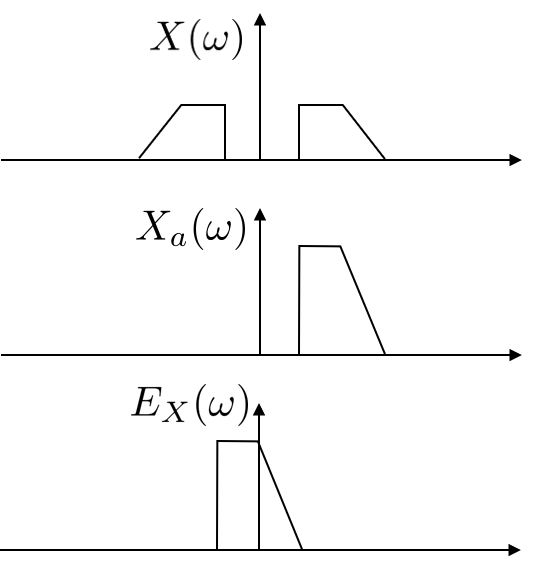
\includegraphics[width=0.3\textwidth]{img/analy_env.png}
\end{figure}


L'enveloppe complexe est $e_x(t)$ :
\begin{equation*}
\begin{split}
E_x(\omega) &= X_a(\omega + \omega_0) \\
e_x(t) &= e^{-j\omega_0t} x_a(t) \\
\end{split}
\end{equation*}


\section{Composantes de Rice}

$$ e_x(t) = x_1(t) - jx_2(t) $$

\begin{multicols}{2}
\begin{equation*}
\begin{split}
x_1(t) &= \Re{[e_x(t)]} \\
&= \Re{[e^{-j\omega_0t}x_a(t)]} \\
&= \Re{[e^{-j\omega_0t} (x(t)+ j \hat{x}(t))]} \\
&= x(t) cos(\omega_0t) + \hat{x}(t) sin(\omega_0t)
\end{split}
\end{equation*}

\begin{equation*}
\begin{split}
x_2(t) &= -\Im{[e_x(t)]} \\
&= -\Im{[e^{-j\omega_0t}x_a(t)]} \\
&= -\Im{[e^{-j\omega_0t} (x(t)+ j \hat{x}(t))]} \\
&= x(t) sin(\omega_0t) - \hat{x}(t) cos(\omega_0t)
\end{split}
\end{equation*}

\end{multicols}

\begin{equation*}
\begin{split}
x(t) &= \Re{[x_a(t)]} \\
&= \Re{[e^{j\omega_0t}e_x(t)]} \\
&= \Re{[e^{j\omega_0t} (x_1(t)- j x_2(t))]} \\
&= x_1(t) cos(\omega_0t) + x_2(t) sin(\omega_0t)
\end{split}
\end{equation*}

On voit donc que tout signal à spectre étroit peut-être vu comme un signal obtenu par la modulation de deux porteuses en quadrature ($sin$ et $cos$) par des signaux $x_1(t)$ et $x_2(t)$ , les composantes de Rice.\\

Voici comment obtenir ces composantes en pratique :

\begin{align*}
2x(t)cos(\omega_0t) &= 2x_1(t)cos^2(\omega_0t) + 2x_2(t)sin(\omega_0t)cos(\omega_0t) \\
&= x_1(t)+ \underbrace{x_1(t)cos(2\omega_0t)+x_2(t)sin(2\omega_0t)}_{filtre}
\end{align*}

\begin{Figure}
    \centering
    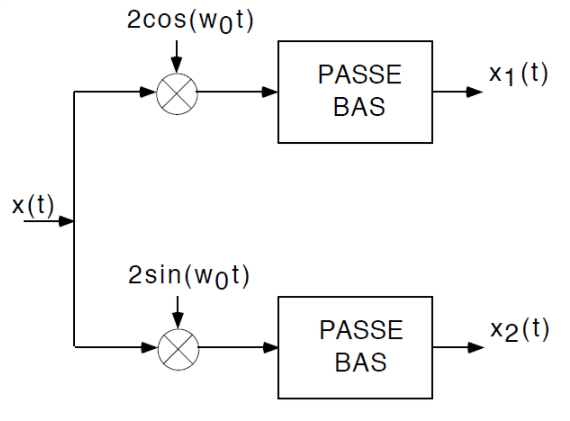
\includegraphics[width=0.3\textwidth]{img/LPF.png}
\end{Figure}


\section{Représentation en coordonnées polaires}

\begin{align*}
e_x &= a_x(t)e^{j\phi_x(t)} \\
x(t) &= a_x(t) cos[\omega_0t + \phi_x(t)] 
\end{align*}

%\newpage

\section{Lien entre les composantes I-Q et $E_x$}


\begin{multicols}{2}
\begin{equation*}
\begin{split}
x_1(t) &= \Re{[e_x(t)]} \\
&= [e_x(t) + e_x^*(t)]/2 \\
X_1(\omega) &= \frac{ E_x(\omega) + E_x^*(-\omega)}{2} \\
\vspace{1cm}
x_2(t) &= -\Im{[e_x(t)]} \\
&= -[e_x(t) - e_x^*(t)]/2j \\
X_2(\omega) &= -\frac{E_x(\omega) - E_x^*(-\omega)}{2j} \\
\end{split}
\end{equation*}

%\vfill\null
%\columnbreak

\begin{equation*}
\begin{split}
E_x(\omega) &= E_{x,p}(\omega) + E_{x,i}(\omega) 
\footnote{Les indices $p$ et $i$ font référence aux parties paires et impaires des enveloppes complexes.}
\\
E_{x,p}(\omega) &= E_{x,p}^*(-\omega) \\
E_{x,i}(\omega) &= - E_{x,i}^*(-\omega) \\
E_{x,p}(\omega) &= \frac{E_{x}(\omega)+E_{x}^*(-\omega)}{2} \\
E_{x,i}(\omega) &= \frac{E_{x}(\omega)-E_{x}^*(-\omega)}{2} \\
\end{split}
\end{equation*}

\end{multicols}

$$\rightarrow E_{x,p}(\omega) = X_1(\omega) \hspace{2.5cm} \rightarrow E_{x,i}(\omega) = -jX_2(\omega)$$

\section{Énergie}

\begin{align*}
\mathcal{E} &= \int_{-\infty}^{\infty} x^2(t) dt \\
&= \int_{-\infty}^{\infty} a_x^2(t) cos^2[\omega_0t+\phi_x(t)]dt \\
&= \int_{-\infty}^{\infty} a_x^2(t) \frac{1}{2} [1+cos(2\omega_0t+2\phi_x(t))]dt \\
&\simeq \frac{1}{2} \int_{-\infty}^{\infty} a_x^2(t) dt 
\end{align*}

\section{Système de types passe bande}

Les filtrages suivants sont équivalents :
\begin{itemize}
\item Process $x(t)$ avec $h(t)$
\item Process $x_a(t)$ avec $h_a(t)/2$
\item Process $e_x(t)$ avec $e_h(t)/2$
\end{itemize}

\begin{Figure}
    \centering
    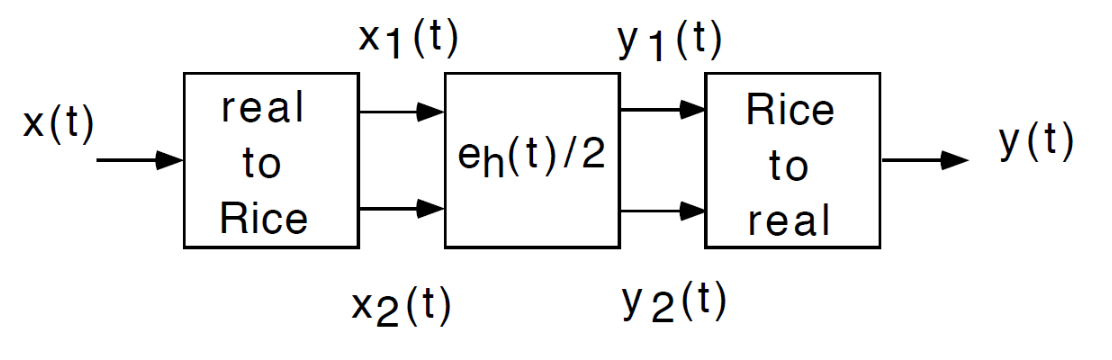
\includegraphics[width=0.5\textwidth]{img/BPSYS.png}
\end{Figure}


\part{Modulations analogiques}

\textbf{\underline{NB}:} phase instantanée $\theta \neq \omega.t = \int \omega(\tau) d\tau$

\section{Modulation en amplitude}


\subsection{Modulation DSB}

$s(t) = A_c[ 1+ \overbrace{k_a}^{\mathclap{\text{taux de modulation}[V^{-1}]}} m(t) ] cos(\omega_ct)
\hspace{3cm}
c(t) = A_c cos(\omega_ct)$ \\

pour éviter la surmodulation : $\left| k_a m(t) \right| \leq 1 \hspace{1cm}$ il faut aussi que :
$f_c >> W$\footnote{on aura au détecteur de crête : $W << \frac{1}{R_1C_1}<<f_0$}


\begin{multicols}{2}

\begin{Figure}
    \centering
    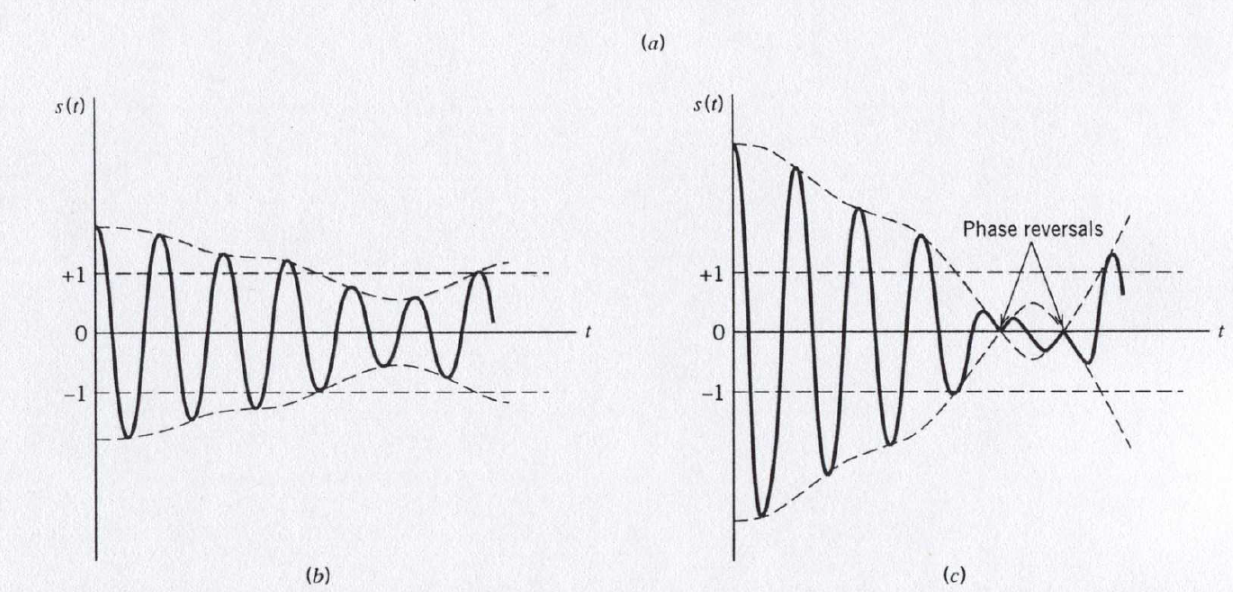
\includegraphics[width=\textwidth]{img/surmod.png}
\end{Figure}

\vfill \null
\columnbreak 

\begin{Figure}
    \centering
    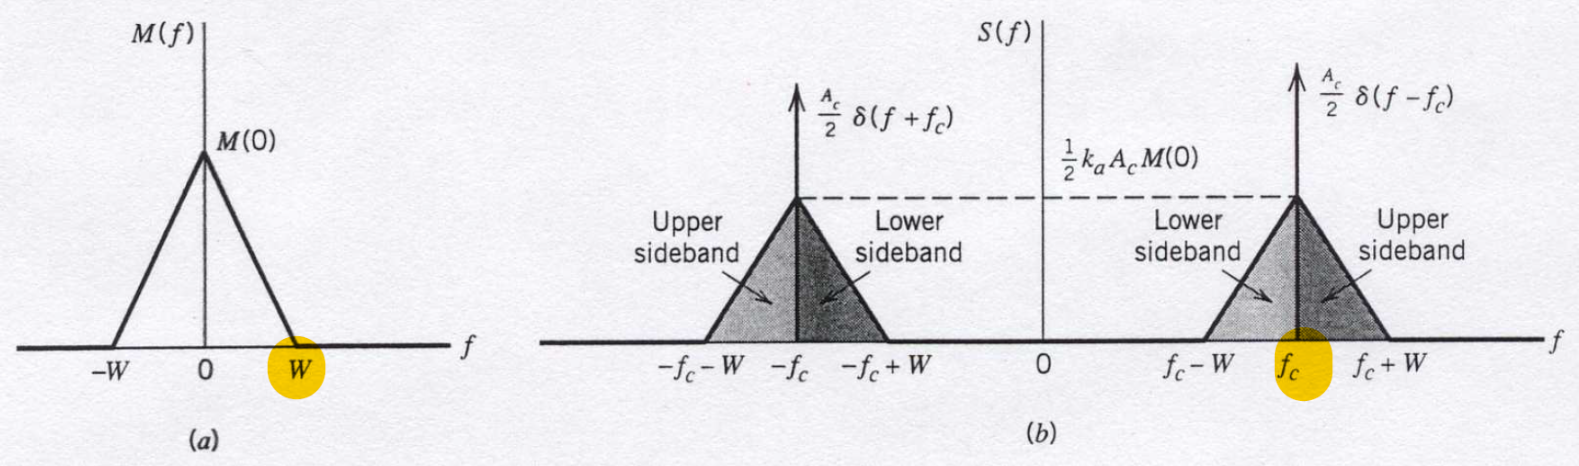
\includegraphics[width=\textwidth]{img/fcW.png}
\end{Figure}

\end{multicols}

\subsubsection*{Puissance}

\begin{align*}
P(t_0,T) &= \frac{1}{T} \int_{t_0}^{t_0+T} s^2(t)dt \\
&= \frac{1}{T} \int_{t_0}^{t_0+T} A_c^2[1+k_m(t)]^2 cos^2(\omega_ct)dt \\
&= \frac{1}{T} \int_{t_0}^{t_0+T} A_c^2[1+k_m(t)]^2 0.5[ \underbrace{1+cos(2\omega_ct)]}_{\mathclap{\omega_c >> W \rightarrow\text{contibution négligeable}}}dt  \\
&\simeq \frac{1}{T} \int_{t_0}^{t_0+T} \frac{A_c^2}{2}[1+k_m(t)]^2\\
&= \frac{A_c^2}{2} + 2 \times \frac{A_c^2}{2} \frac{1}{T}k_a \int_{t_0}^{t_0+T} m(t) dt \\
&+ \frac{1}{T} \frac{A_c^2}{2} k_a^2 \times \int_{t_0}^{t_0+T} m^2(t) dt
\end{align*}

Si $m(t)$ est une sin d'amplitude 1, on a $\frac{A_c^2}{2}$ consommé par la porteuse, et $\frac{A_c^2}{2} \frac{k_a^2}{2}$ pour le signal d'information.\\
Si $k_a =1$ la porteuse consomme le double du signal d'info ! Cette modulation est inefficace en terme de puissance et de bande passante puisqu'on passe de $W$ à $2W$ en bande utilisée !


\subsection{Modulation DSB-SC}

$s(t) = A_cm(t)cos(\omega_ct) \hspace{5cm} S_{LO} = A_c'cos(\omega_ct+\phi]$\\

On a donc un changement de phase à chaque fois que le signal $m(t)$ passe par 0 ce qui nécessite  une détection cohérente de phase. Ceci se fait à l'aide d'un local oscillator L.O.):
\begin{align*}
s(t)\times s_{LO} &= A_c A_c' \ m(t)\ cos(\omega_ct) \ cos(\omega_ct+\phi)\\
&= \frac{A_c A_c'}{2} \ m(t)\ [cos(\phi) + \underbrace{cos(2\omega_ct+\phi)}_{\mathclap{\text{à filtrer}}}]\footnotemark\\
\hat{m}(t) &= \frac{A_c A_c'}{2} \ m(t)\ cos(\phi) \hspace{2cm} \phi = \theta_1 - \theta_2 = \phi_{m(t)} - \phi_{L.O}
\end{align*}
\footnotetext{
\begin{align*}
2\ cos^2a &= 1+cos(2a) \hspace{6.6cm}
cos(a)\ cos(b) &= \frac{1}{2}[cos(a-b)+cos(a+b)]\\
sin(a)\ sin(b) &= \frac{1}{2}[cos(a-b)-cos(a+b)]\hspace{4.5cm}
sin(a)\ cos(b) &= \frac{1}{2}[sin(a-b)+sin(a+b)]\\
\end{align*}
}

\subsubsection*{Boucle de Costas}
La boucle de Costas est un récepteur dont l'objectif est d'assurer une démodulation cohérente du signal reçu.
\begin{multicols}{2}
signal reçu :
$$ s(t) = A_c\ m(t)\ cos(\omega_ct)$$

\vfill\null
\columnbreak

signaux produits localement:
\begin{align*}
s_I(t) &= A_c'\ cos(\omega_ct + \phi)\\
s_Q(t) &= A_c'\ sin(\omega_ct + \phi)
\end{align*}

\end{multicols}
\noindent  $s(t) \times s_I(t)$ après filtrage $=\hat{m}_I(t) = \frac{A_c\ A_c'}{2}m(t)\ cos(\phi)$\\ 
$s(t) \times s_Q(t)$ après filtrage $=\hat{m}_Q(t) = \frac{A_c\ A_c'}{2}m(t)\ sin(\phi)$\\

L'estimation du décalage de phase (phase discriminator) peut se faire par exemple
en calculant le produit $m_I (t) \times m_Q(t)$ et en intégrant ce produit. On obtient
$$ \hat{m}_Q(t) \times \hat{m}_I(t) = \frac{(A_c\ A_c')^2}{8}\ m^2(t) sin(2\phi) $$
\begin{multicols}{2}
Après intégration temporelle, on obtient un signal proportionnel à $sin(2\phi)$.L'on voit donc que si $\phi = 0$ la boucle n’opère pas de correction, ce qui est bien souhaité. Par contre, s'il y a une erreur de phase, et qu'elle peut être considérée
comme suffisamment petite, le sin peut être linéarisé et le signal d'erreur est
proportionnel à $\phi$. Ce signal attaque un VCO, voltage controlled oscillator. Cet oscillateur a une fréquence naturelle, qui peut être accélérée ou décélérée  par application d'une tension. Ici cette tension est le signal d’erreur.
\vfill\null
\columnbreak
\begin{Figure}
    \centering
    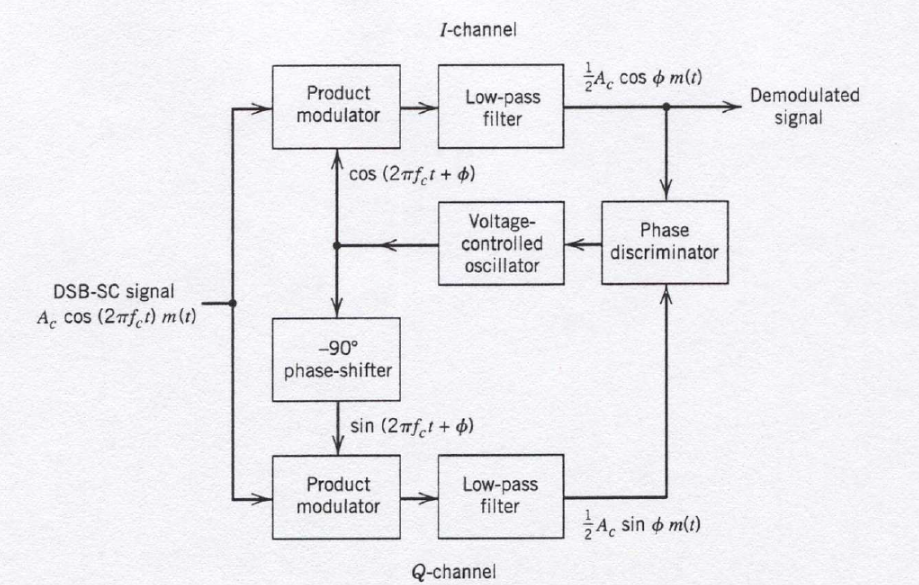
\includegraphics[width=\textwidth]{img/costas.png}
\end{Figure}
\end{multicols}

\subsection{Modulation en quadrature}

C'est aussi la détection cohérente qui permet de moduler deux porteuses en quadrature par des signaux différents, comme montré plus haut. Ce type de modulation permet à deux signaux \textbf{indépendants} d'occuper la même bande
tout en étant séparables. Ce schéma est donc intéressant en ce qui concerne la bande passante.
Le signal modulé est donné par:
$$s(t) = A_c\ m_I(t)\ cos(\omega_ct)+A_c\ m_Q(t)\ sin(\omega_ct)$$
Dans le récepteur, on produit deux porteuses en quadrature à l'aide de l'OL, correspondant à $s_I(t)$ et $s_Q(t)$ donnés ci-dessus.
\begin{multicols}{2}
\noindent
\begin{align*}
s(t)\ s_I(t) &= \frac{A_c\ A_c'}{2}\ m_I(t) [1+cos(2\omega_ct)] \\
&+ \frac{A_c\ A_c'}{2}\ m_Q(t)\ sin(2\omega_ct)\\
&\downarrow\\
\hat{m}_I(t) &= \frac{A_c\ A_c'}{2}\ m_I(t)
\end{align*}
%\vfill\null
\columnbreak
\begin{align*}
s(t)\ s_Q(t) &= \frac{A_c\ A_c'}{2}\ m_I(t)\ sin(2\omega_ct) \\
&+ \frac{A_c\ A_c'}{2}\ m_Q(t) [1+cos(2\omega_ct)] \\
&\downarrow\\
\hat{m}_Q(t) &= \frac{A_c\ A_c'}{2}\ m_Q(t)
\end{align*}
\end{multicols}

Lorsque le signal $m_Q(t)$ n'est pas indépendant de $m_I(t)$, il n'est plus nécessaire d'occuper $2W$ en largeur de bande et on peu donc avoir recours à la SSB ou la VSB en pratique.

\subsection{Modulation SSB}

Pour qu'une modulation SSB soit possible, il faut que le spectre du signal modulant ne s'étende pas jusqu'au DC.\\ On ne garde qu'un seul lobe en prenant le signal analytique (gauche | droite ):
$$m_a'(t) = m(t) - j\hat{m}(t) \hspace{3cm} m_a(t) = m(t) + j\hat{m}(t)$$
On transporte ensuite la bande latérale droite vers une fréquence porteuse positive et la bande latérale gauche vers l'opposé de cette fréquence ( modulation SSB du lobe de droite). Ou on peut aussi choisir de transporter la bande latérale gauche vers une fréquence porteuse négative et la bande latérale droite vers l'opposé de cette fréquence (modulation SSB du lobe de gauche)
\begin{multicols}{2}
\noindent
\begin{align*}
s_-(t) &= m_a'(t)\ e^{-j\omega_ct} \\
s_-(t) &= m_a(t)\ e^{-j\omega_ct}\\
\end{align*}
%\vfill\null
\columnbreak
\begin{align*}
s_+(t) &= m_a(t)\ e^{j\omega_ct}\\
s_+(t) &= m_a'(t)\ e^{j\omega_ct}
\end{align*}
\end{multicols}
\vspace{-7ex}
Le signal SSB complet est donc donné par :
\begin{align*}
s_{sup}(t) &= m_a'(t)\ e^{-j\omega_ct}+ m_a(t)\ e^{j\omega_ct} \\
&= 2\ m(t)\ cos(\omega_ct) - 2\ \hat{m}(t)\ sin(\omega_ct) \\
s_{inf}(t) &= m_a(t)\ e^{-j\omega_ct}+ m_a'(t)\ e^{j\omega_ct} \\
&= 2\ m(t)\ cos(\omega_ct) + 2\ \hat{m}(t)\ sin(\omega_ct)
\end{align*}

\subsection{Modulation VSB}

\subsubsection*{modulation:}
Si le spectre du signal s'étend jusqu'au DC et qu'on veut malgré tout ne transmettre qu'un lobe, on ne sera pas capable de concevoir un filtre à pente infinie à la fréquence nulle. On va donc transmettre un presque l'entièreté d'une bande latérale plus un résidu de l'autre, avec pour objectif de compenser ou reconstruire ce qui manque du premier lobe. On synthétise donc un signal DSB-SC qu'on passe ensuite dans un filtre particulier. Comme le filtre est $\mathbb{R}$, on a la symétrie conjuguée en fréquentiel :$H_+(\omega) = H_-^*(-\omega)$

\begin{Figure}
    \centering
    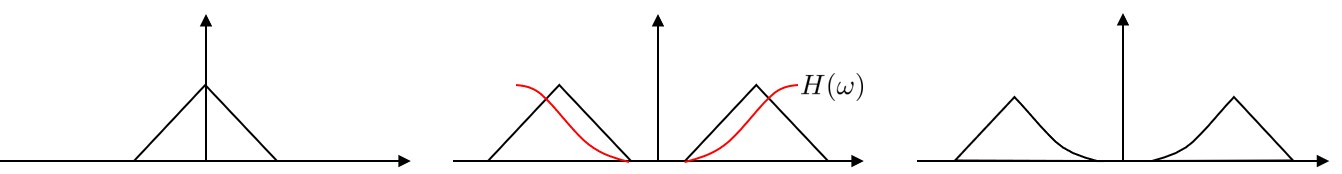
\includegraphics[width=0.8\textwidth]{img/moduVSB.jpg}
\end{Figure}

On aura :

\begin{align*}
s_+(t) &= s(t) + j \hat{s}(t) \\
s_-(t) &= s(t) - j \hat{s}(t) \\
\end{align*}


\subsubsection*{démodulation}

Il faut ramener les 2 triangles courbés au centre pour obtenir le triangle de départ. On a le signal VSB $S(\omega)$ les deux triangles courbés et $M(\omega)$ le signal modulant (le triangle de départ).  


\begin{multicols}{3}
\noindent
triangles de gauche et droite :
\begin{align*}
S_+(\omega) &= 2M(\omega-\omega_c)\ H_+(\omega) \\
S_-(\omega) &= 2M(\omega+\omega_c)\ H_-(\omega) \\
\end{align*}
\vfill\null
\columnbreak
triangles au centre :
\begin{align*}
S_+(\omega) &= 2M(\omega)\ H_+(\omega+\omega_c) \\
S_-(\omega) &= 2M(\omega)\ H_-(\omega-\omega_c) \\
\end{align*}
\vfill\null
\columnbreak
résultat :
\begin{align*}
&= 2M(\omega)\ \left( H_+(\omega+\omega_c) + H_-(\omega-\omega_c) \right) \\
&= 2M(\omega)\ \left( H_+(\omega+\omega_c) + H_+^*(\omega-\omega_c) \right) \\
\end{align*}
\vfill\null

\end{multicols}
\vspace{-7ex}
Pour récupérer $M(\omega)$ il faut donc que $\left[ H_+(\omega+\omega_c) + H_+^*(\omega-\omega_c) \right] = 1$.\\
Dans le domaine temporel, on aura :
\begin{align*}
m'(t) &= s_+(t)\ exp(-j\omega_c t) + s_-(t)\ exp(j\omega_ct)\\
&= 2\ s(t)\ cos(\omega_ct) + 2\ \hat{s}(t)\ sin(\omega_ct)
\end{align*}

\subsubsection*{Synthèse VSB en bande de base}

\underline{Idée}: Plutôt que de prendre le signal DSB-SC  $m(t) + j \hat{m}(t)$ (pour la partie de droite ici), de le passer dans un filtre $H(\omega)$ et d'obtenir $s_{VSB}(t)$, on produit un signal $m_q(t)$ lié à $m(t)$ tel que $m(t) + j m_q(t)$ donne le même résultat qu'à la sortie du filtre:
$$ M(\omega-\omega_c) + j H_q(\omega - \omega_c)\  M(\omega - \omega_c) = 2H_+(\omega)M(\omega-\omega_c)$$
$$ H_q(\omega) = \frac{[2H_+(\omega_c+\omega)-1]}{j} $$

On aura donc bien :
\begin{align*}
s(t) &= [m(t)+j m_q(t)]exp^{j\omega_ct}+[m(t)-j m_q(t)]exp^{-j\omega_ct}\\
&= 2m(t)\ cos(\omega_ct) - 2m_q(t)\ sin(\omega_ct)
\end{align*}

\subsection*{Télévision}

%%TODO
Systèmes NTSC \& PAL $\rightarrow$ pages 95 à 100 du syllabus\\


\subsection{Effet du bruit}

\begin{Figure}
    \centering
    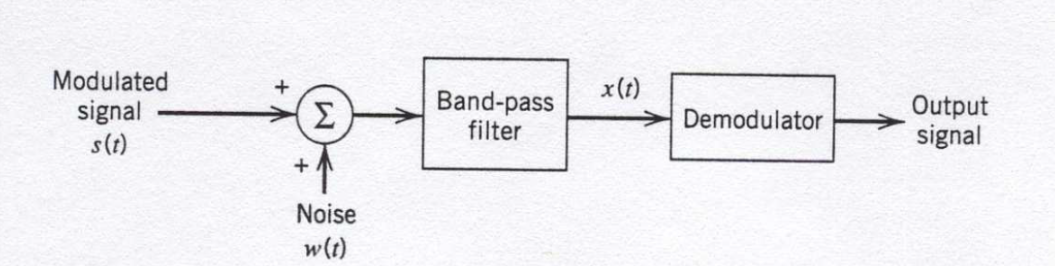
\includegraphics[width=0.6\textwidth]{img/struct.png}
\end{Figure}

Le bruit est supposé blanc et de densité spectrale bilatérale $\frac{N_0}{2}$. Le filtre a pour but de limiter le bruit à l'entrée du démodulateur, il est supposé idéal et centré sur la $f$ de la porteuse et est de largeur $B$ celle du signal modulé. Le signal qui arrive au démodulateur est de la forme :
$$x(t) = s(t) + n(t)\hspace{3cm} n(t) = n_I(t)\ cos(2\pi f_c t)+n_Q(t)\ sin(2\pi f_c t)$$ 
On peut définir plusieurs rapports signal-à-bruit:
\begin{itemize}
\item $SNR_i$ : rapport de la $P_{moy}$ du signal modulé à la $P_{moy}$ du bruit.
\item $SNR_o$ : rapport de la $P_{moy}$ du signal démodulé en sortie à la $P_{moy}$ du bruit.
\item $SNR_c$ : rapport de la $P_{moy}$ du signal à la $P_{moy}$ du bruit \textit{dans la bande du message (channel)}, tous deux mesurés à l'entrée du récepteur. 
\end{itemize}

Enfin on appelle le gain de rapport signal-à-bruit : $G_m = \frac{SNR_o}{SNR_c}$

\subsection*{Modulation DSB-SC}
\noindent
$s(t) = A_c\ m(t)\ cos(2\pi f_c t)$\\
$x(t) = A_c\ m(t)\ cos(2\pi f_c t)+ n_I(t)\ cos(2\pi f_c t)+n_Q(t)\ sin(2\pi f_c t)$\\
On suppose que le signal modulant est stationnaire de densité $S_m(\omega)$, limité à la bande $W$. Sa puissance est donnée par :
$$ P_m = \frac{1}{2\pi}\int_{-W}^{W}S_m(\omega)d\omega $$
Pour calculer \textbf{la puissance du signal modulé}, il nous faut la covariance. Nous devons donc le rendre aléatoire :
\vspace{-4ex}
\begin{align*}
s_{\theta} &= A_c\ m(t)\ cos(2\pi f_c t+ \phi)\\
C_{s_{\theta}}(\tau) &= \textbf{E}[s_{\theta}(t+\tau)\ s_{\theta}(t)]\\
&= A_c^2\ \textbf{E}\left( m(t+\tau)\ m(t) \right)\ cos(2\pi f_c (t+\tau)+\theta)\ cos(2\pi f_c t + \theta) \\
&= \frac{A_c^2}{2}C_m(\tau)\ \{ cos[2\pi f_c \tau] + cos[2\pi f_c(2t + \tau) + 2\theta ]\}\\
&\text{On supprime le conditionnement en intégrant sur } \theta\\
C_s(\tau) &= \frac{A_c^2}{2}C_m(\tau)\ cos[2\pi f_c \tau]\\
P_s &= C_s(0) = \frac{A_c^2}{2}P_m
\end{align*}

La puissance du bruit dans la bande du message est donnée par : $2W \times N_0/2$
$$SNR_c = \frac{A_c^2\ P_m}{2N_0W}$$

%\newpage	

A la sortie du démodulateur cohérent pour $n_I(t)$:
\begin{align*}
x(t)cos(2\pi f_c t) &= s(t)cos(2\pi f_c t) + n(t) cos(2\pi f_c t)\\
\text{On obtient :} \hspace{2cm} m'(t) &= \underbrace{\frac{A_c}{2} m(t)}_{\text{1 - utile}} + \underbrace{\frac{n_I(t)}{2}}_{\text{2 - bruit}}
\end{align*}

On peut ne pas se soucier des $\frac{1}{2}$ car le rapport SN ne change pas si on multiplie la partie utile et le bruit $\times 2$. 

\begin{enumerate}
\item $P_u = A_c^2\ P_m$
\item On a $\gamma_{n_I}(\omega) = \gamma_{\mathcal{E}}(\omega)/2 = 4\ \gamma_n(\omega-\omega_0)/2 = 2\ \frac{N_0}{2} = N_0 $\\
Le filtre va avoir une largeur $2W$ autour de $f_c$ donc $P_b = 2WN_0$\\
\underline{NB} : on aurait pu le deviner car on sait que les composantes de Rice ont la même puissance que le signal dont elles proviennent.
$$\text{On obtient :} \hspace{2cm} SNR_o = \frac{A_c^2\ P_m}{2N_0W}$$
$$\text{Donc :} \hspace{2cm} G_{m,DSB-SC} = 1$$
\end{enumerate}

\subsection*{Modulation SSB}

On aura 
\begin{align*}
G_{m,SSB} &= 1\\
\frac{SNR_o}{SNR_i} &= 1
\end{align*}

Ceci vient du fait que la bande RF a la même largeur que la bande de base, $2W$ et que le démodulateur SSB se contente de ramener la bande latérale située autour de la porteuse, autour de 0.

\subsection*{Détection d'enveloppe}

\begin{multicols}{2}
\noindent
$s(t) = A_c[1+k_a\ m(t)]\ cos(2\pi f_c t)\vspace{0.2cm}$\\
$P_s = \underbrace{\frac{A_c^2}{2}}_{\text{porteuse}}+ \underbrace{\frac{A_c^2}{2} k_a^2\ P_m}_{\text{utile}}$

\vfill\null
\columnbreak
\noindent

Le signal reçu est :
\noindent
\begin{align*}
x(t) &= s(t) + n(t)\\
&= \{A_c[1+k_a m(t)]+n_I(t)\}\ cos(2\pi f_c t)\\
&+ n_Q(t)\ sin(2\pi f_c t)
\end{align*}

\end{multicols}

l'amplitude instantanée : $a_x^2(t) = \{A_c[1+k_a m(t)]+n_I(t)\}^2 + n_Q(t)^2$\\

Lorsque le signal a un bon rapport SN, on peut négliger le $n_(t)$ et obtenir :
$$a_x(t) \simeq A_c[1+k_a m(t)]+n_I(t)$$
\begin{align*}
\text{On obtient :} \hspace{1cm} SNR_o &= \frac{A_c^2\ k_a^2\ P_m}{2N_0W} \hspace{1cm} \underline{\text{valable pour un bon rapport SN}}\\
\text{Ou encore :} \hspace{1cm} SNR_c &= \frac{A_c^2}{2}\frac{1+k_a^2\ P_m}{N_0W} \\
\text{Dès lors :} \hspace{1cm} G_m &= \frac{k_a^2\ P_m}{|1+k_a^2\ P_m|} < 1
\end{align*}

%\newpage

\subsection{L'effet de seuil}

\begin{align*}
SNR_o &= G_m\ SNR_i \\
10 \ log\  SNR_0 &= 10 \ log\  G_m + 10\ log \ SNR_i
\end{align*}
Ceci est valable pour un $SNR_i$ supérieur à une valeur seuil :

\begin{multicols}{2}

\begin{Figure}
    \centering
    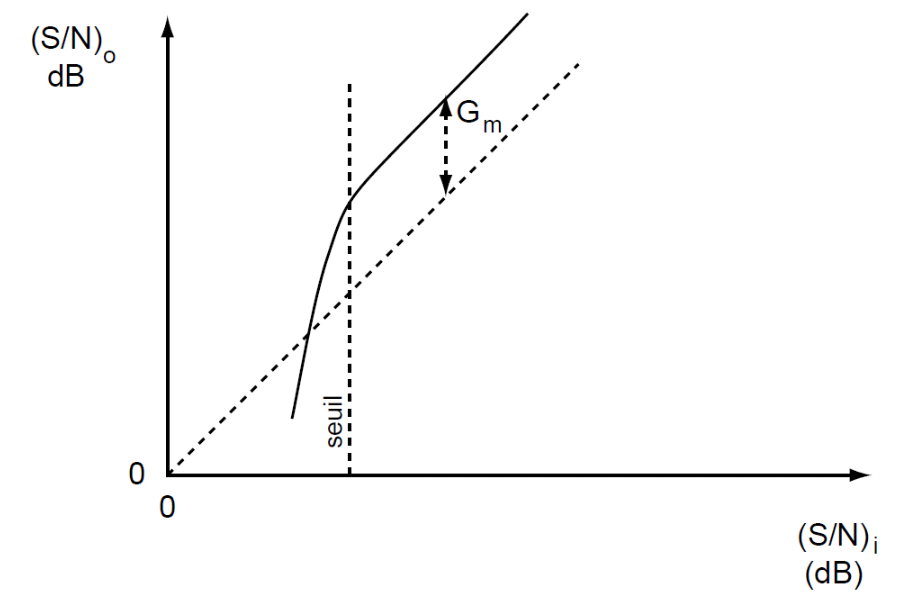
\includegraphics[width=0.8\textwidth]{img/seuil.png}
\end{Figure}
\vfill\null
\columnbreak
\noindent

Le seuil fait référence à la valeur de $SNR_i$ en dessous de laquelle les performances se dégradent plus rapidement que simplement proportionnellement au rapport signal-à-bruit. \textit{Tout détecteur non linéaire est caractérisé par un tel effet. Ce n'est pas le cas des détecteurs cohérents.}

\end{multicols}

\subsection{Changement de fréquence}

\begin{Figure}
    \centering
    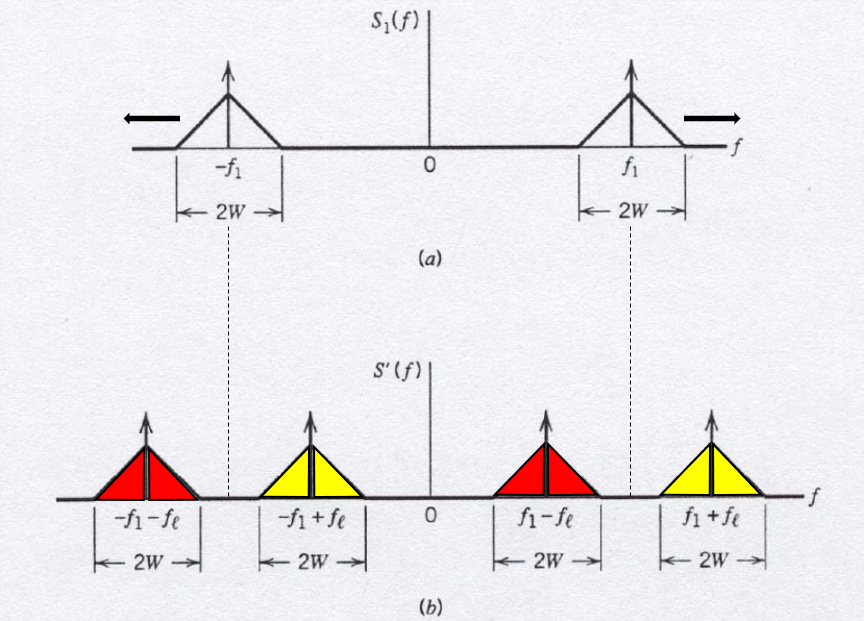
\includegraphics[width=0.5\textwidth]{img/chgtf.png}
\end{Figure}

Cette opération p-ê réalisée au moyen d'un \textit{mélangeur}. Si l'on veut déplacer un signal d'une fréquence $f_1$ vers $f_2 = f_1 + f_l$, on obtient bien le résultat escompté à savoir le signal transporté en $f_1+f_l$, mais on obtient aussi un signal autour de $f_1 - f_l$ et bien entendu tous les signaux correspondant dans les fréquences négatives !\\
On peut avoir recours à un filtre passe bas servant à éliminer les composantes fréquentielles situées autour de $f_1 - f_l = f_2 - 2f_l$ dite \textit{fréquence image}.\\
Il faut aussi s'assurer que les plages de fréquences ne sont pas occupées pas d'autres signaux qui pourraient venir empiéter sur les signaux utiles.

\section{Modulations angulaires}


Les modulations angulaires permettent une amélioration du rapport SNR en augmentant la largeur de bande utilisée, ce qu'on ne pouvait pas faire avec les modulations AM.
\begin{itemize}
\item Fréquence instantanée: $f_i(t) = \frac{1}{2\pi}\frac{d\theta_i(t)}{dt}$
\item Enveloppe complexe : $e_s(t) = A_c e^{j(\theta_i(t)-\omega_0.t)}$
\end{itemize}
Il existe deux types de modulations angulaires:\\

\noindent \textcolor{red}{modulation de phase}: phase instantanée $\theta_i(t) = 2\pi f_ct+k_pm(t)$\\
$k_p$ est la sensibilité du modulateur $\left[ \frac{rad}{V}\right]$ 
$$s(t) = A_c \ cos[2\pi f_c t + k_p m(t) ] $$

\noindent \textcolor{red}{modulation de fréquence}: $f_i(t) = f_c + k_f m(t)$
$$s(t) = A_c \ cos[2\pi f_c t + 2\pi k_f \int_0^t m(\tau) d\tau ] $$
exemple d'une modulation par un signal simple ton:
\begin{align*}
m(t) &= A_m cos(2\pi f_m t)\\
f_i(t) &= f_c + k_f\ A_m cos(2\pi f_mt) \\
&= f_c + \Delta f \ cos(2\pi f_mt) 
\end{align*}
$\Delta f = k_f\ A_m$ est appelée la déviation de fréquence, proportionnelle à l'amplitude du signal modulant et indépendante de la fréquence de ce signal modulant. La fréquence instantanée oscille donc autour de $f_c \pm\Delta f$.
\begin{align*}
\theta_i(t) &= 2\pi f_c t + 2\pi k_f \int_0^t m(\tau) d\tau \\
&= 2\pi f_c t + 2\pi k_f A_m \int_0^t cos(2\pi f_m \tau) d\tau \\
&= 2\pi f_c t + 2\pi \frac{k_f A_m}{2\pi f_m}sin(2\pi f_m t)\\
&= 2\pi f_c t + \frac{\Delta f}{f_m}.sin(2\pi f_m t)
\end{align*}
$\beta = \Delta f/f_m$ est appelé \textbf{indice de modulation FM}. $ \theta_i(t) = 2\pi f_c t + \beta.sin(2\pi f_m t)$ d'où $\beta\ [rad]$ est l'écart maximal que peut avoir la phase instantanée par rapport à la phase de la porteuse non-modulée.
$$s(t) = A_c \ cos[2\pi f_c t + \beta sin(2\pi f_m t)]$$


\subsection{FM à bande étroite ($\beta << 1$):}
\begin{align*}
s(t) &= A_c cos[2\pi f_c t]\ \underbrace{cos[\beta\ sin(2\pi f_mt)]}_{\simeq 1} - A_c sin[2\pi f_ct]\ \underbrace{ sin[\beta\ sin(2\pi f_m t)]}_{\simeq \beta\ sin(2\pi f_m t)} \\
&\simeq  A_c cos[2\pi f_c t] - A_c\ \beta\ sin(2\pi f_m t)\ sin[2\pi f_ct]
\end{align*}

On remarque que cette forme de modulation est proche de la modulation DSB. On retrouve d'ailleurs le même effet de décalement que dans cette modulation sur le spectre du signal modulé :
\begin{figure}[H]
    \centering
    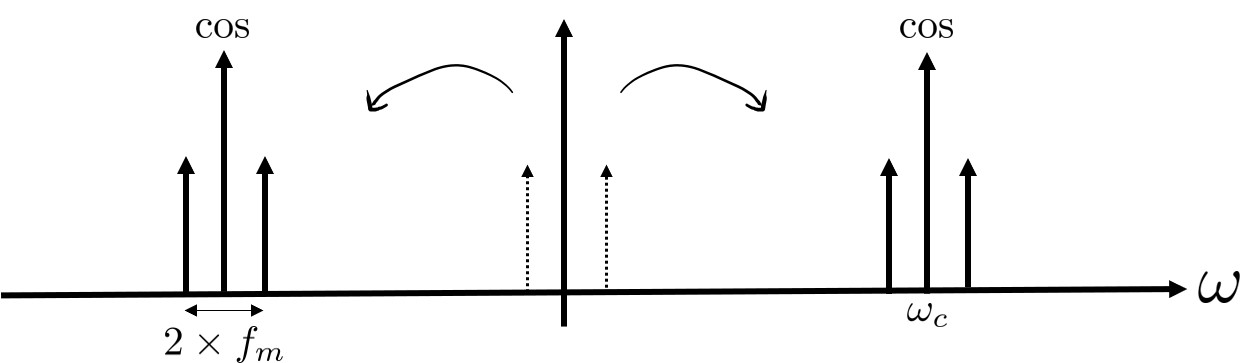
\includegraphics[width=0.9\textwidth]{img/BandeEtroite.jpg}
    \caption{Spectre d'une modulation FM à bande étroite}
    \label{fig : bande etroite}
\end{figure}
Les deux conditions que remplissent les véritables signaux modulés en FM sont :
\begin{itemize}
\item amplitude  $a_c \Perp t$
\item $\theta_s(t) = 2\pi f_c t + \frac{\Delta f}{f_m}.sin(2\pi f_m t)$
\end{itemize}
pour un signal FM à bande étroite, aucune de ces conditions n'est remplie.

\subsection{FM à bande large ($\beta >>  1$):}

$$s(t) = \Re{[A_c e^{j\beta sin(2\pi f_mt)}.e^{2\pi j f_c t}]} $$
On en sort l'enveloppe complexe du signal modulé : $e_s(t) = A_c e^{j\beta sin(2\pi f_mt)}$, un signal périodique que l'on peut décomposer en séries de Fourier, $e_s(t) = \sum_{k=-\infty}^{\infty} A_c J_k(\beta) exp^{2\pi j k f_m t}$. Le signal modulé est donc :
\begin{align*}
s(t) &= \Re{[e_s(t).exp^{2\pi j f_c t}]}\\
&= \Re{[\sum_{k=-\infty}^{\infty} A_c J_k(\beta) exp^{2\pi j k f_m t}.exp^{2\pi j f_c t}]}\\
&= \sum_{k=-\infty}^{\infty} A_c J_k(\beta).cos[2\pi(f_c + k.f_m).t]
\end{align*}
\begin{figure}[H]
    \centering
    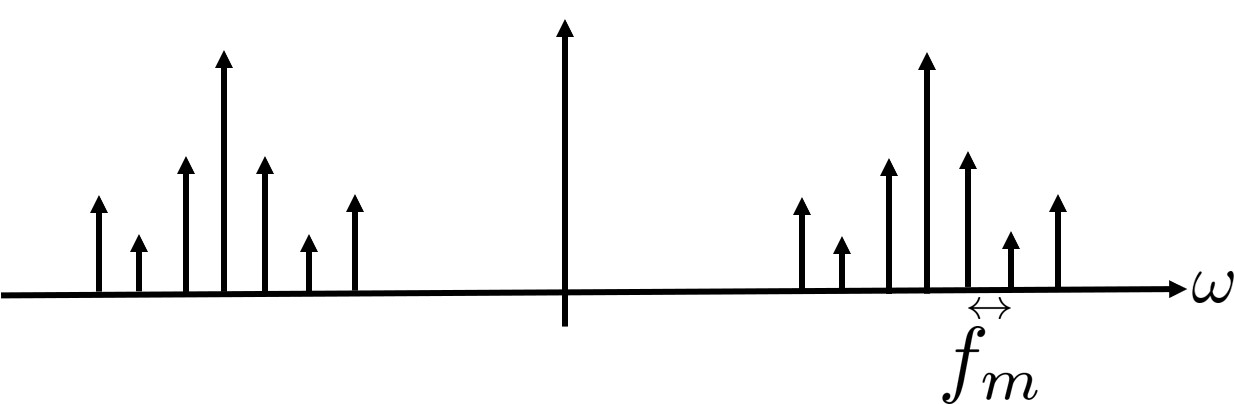
\includegraphics[width=0.9\textwidth]{img/BandeLarge.jpg}
    \caption{Spectre d'une modulation FM à bande large}
    \label{fig : bande large}
\end{figure}
On trouve aussi que les coefficients de Bessel pour des faibles indices de modulation: $J_0(\beta) \simeq 1$ ; $J_1(\beta) \simeq \beta/2$ ; $J_{n>2}(\beta) \simeq 0$ font qu'on retrouvera bien un spectre semblable à celui de la figure \ref{fig : bande etroite}. L'énergie totale comprise dans les différents deltas est aussi \textbf{constante} ! ($\sum_{k=-\infty}^{\infty} J_k^2(\beta) = 1$)\\ 

%\samepage{

\begin{multicols}{2}
\noindent
\begin{Figure}
    \centering
    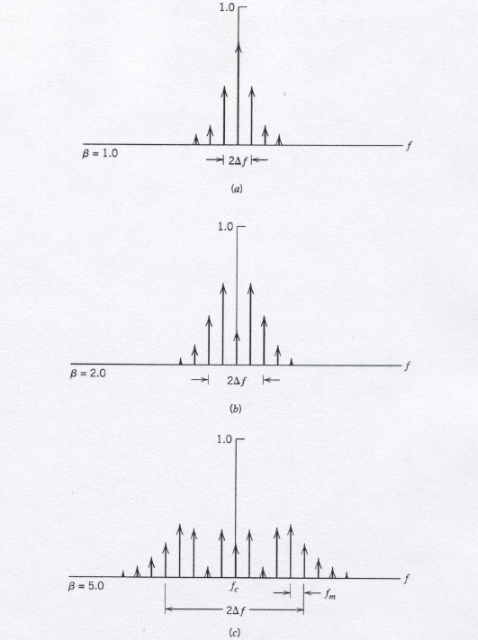
\includegraphics[width=0.7\textwidth]{img/fmFixe.png}
    \captionof{figure}{$f_m$ fixe}
\end{Figure}
\vfill\null
\columnbreak
\noindent
\begin{Figure}
    \centering
    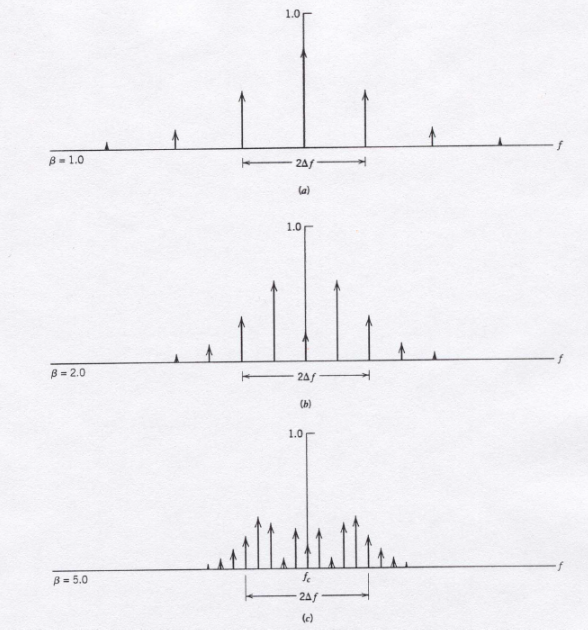
\includegraphics[width=0.7\textwidth]{img/DeltafFixe.png}
    \captionof{figure}{$\Delta f$ fixe}
\end{Figure}
\end{multicols}
%}

On constate donc que pour un signal simple ton, lorsque $\beta \rightarrow \infty$, la bande dépasse très modérément $2\Delta f$. Formule de Carson :
$$ B_T = 2 \underbrace{\Delta f}_{\textbf{!}} + 2 f_m $$
En FM, le spectre du signal modulé n'est pas fortement affecté par le spectre du signal modulant mais par \textbf{l'amplitude} de celui-ci ($\Delta f = k.A_m$) !\\

Si on a pas un signal simple ton, on peut prendre l'approche worst case à l'aide d'un signal simple ton en remplaçant $f_m$ par $W$, la plus haute fréquence observée dans le signal.

\subsubsection*{Déplacer bande :}

Pour centrer la bande autour de $n.f_c$, on utilise une non linéarité ex: $cos^n(x) \rightarrow cos(nx)$.
\begin{align*}
&\underline{Entrée} &&& \underline{Sortie}\\
s(t) &=  A_c \ cos[2\pi f_c t + 2\pi k_f \int_0^t m(\tau) d\tau ]
&&&
v(t) &= A_c' cos[2\pi nf_c t + 2\pi nk_f \int_0^t m(\tau) d\tau ]
\end{align*}

\subsection{Démodulation}
L'organe chargé de la démodulation FM est un discriminateur (on peut aussi utiliser un PLL - phase locked loop) qui va sortir l'information de l'argument sur l'amplitude du signal, que l'on pourra ensuite facilement lire à l'aide d'une détecteur de crête. Il est donc très important que l'amplitude ne soit \textbf{pas modifiée} par autre chôse sinon le signal est corrompu. On sort l'argument en dérivant ($\times j.\omega.cste)$:
\begin{figure}[H]
    \centering
    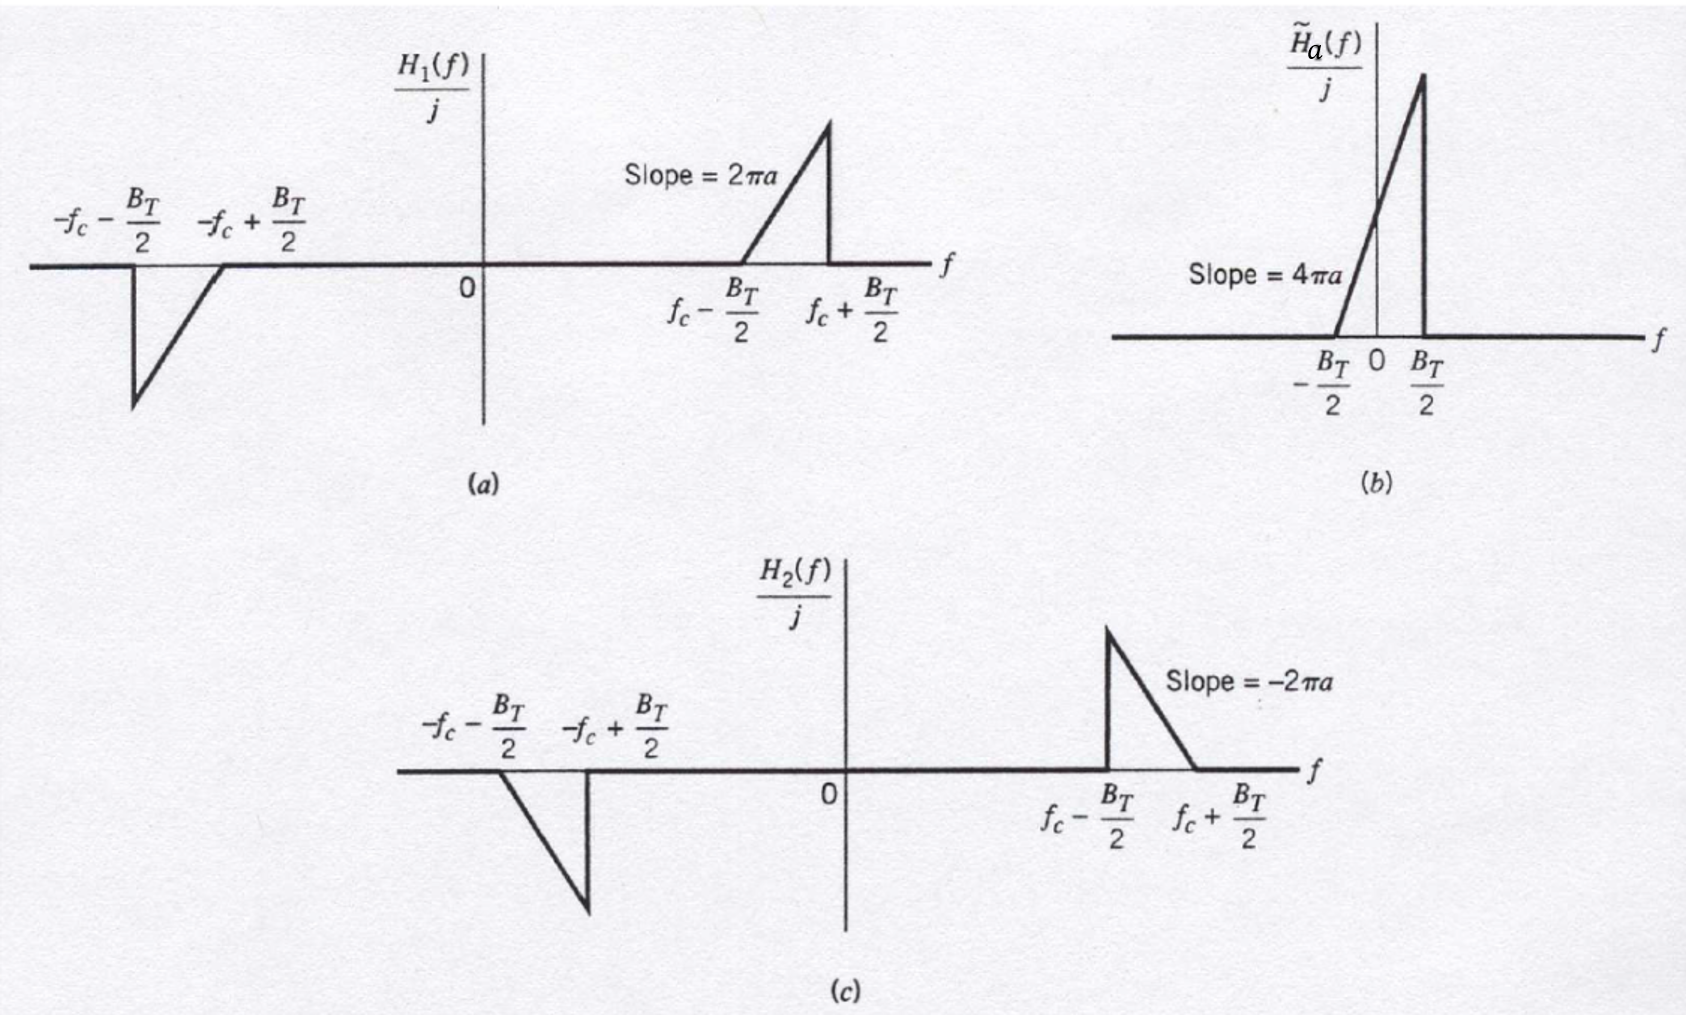
\includegraphics[width=0.7\textwidth]{img/Discri.png}
    \caption{Spectre du discriminateur}
    \label{fig : filtre discri}
\end{figure}

On voit que le filtre revient $\pm$ à multiplier le spectre du signal par $\times j.\omega$ autour sur la bande du signal $s(t)$.\\
Il est important de pouvoir ramener les opérations en bande de base:

\begin{equation}
H_a(f) = 
\left\{
\begin{array}{l}
j4\pi a (f+B_T/2) \\
0
\end{array}
\right.
\begin{array}{l}
si -B_T/2 \leq f \leq B_T/2 \\
sinon
\end{array}
\end{equation}
Enveloppe de $s(t)$ :
\begin{equation}
e_s(t) = A_c exp^{2\pi j k_f \int_0^t m(\tau) d\tau }
\end{equation}
Sortie:
\begin{equation}
E'_s(f) = H(f)E_s(f)/2 = 
\left\{
\begin{array}{l}
j2\pi a (f+B_T/2)E_s(f)\\
0
\end{array}
\right.
\begin{array}{l}
si -B_T/2 \leq f \leq B_T/2 \\
sinon
\end{array}
\end{equation}

Dès lors dans le domaine direct :
\begin{align*}
e'_s(t) &= a.\frac{d e_s(t)}{dt} + j\pi a B_T e_s(t) \\
&= [a2\pi j k_f m(t) + j\pi a B_T ].A_c exp^{2\pi j k_f \int_0^t m(\tau) d\tau}
\end{align*}
La sortie réelle est :
\begin{align*}
s_1(t) &= \Re{[e_s'(t) exp^{2\pi j f_ct}]} \\
&= \underbrace{\pi a B_T [1+2 k_f m(t)/B_T]A_c} cos[ 2\pi f_c t + 2\pi k_f \int_0^t m(\tau) d\tau +\pi/2]
\end{align*}
On voit donc ici qu'il est primordial que l'amplitude ne dépende pas du temps. On fera en sorte que ce soit le cas à l'aide d'un limiteur. La chaine considérée est :
\begin{figure}[H]
    \centering
    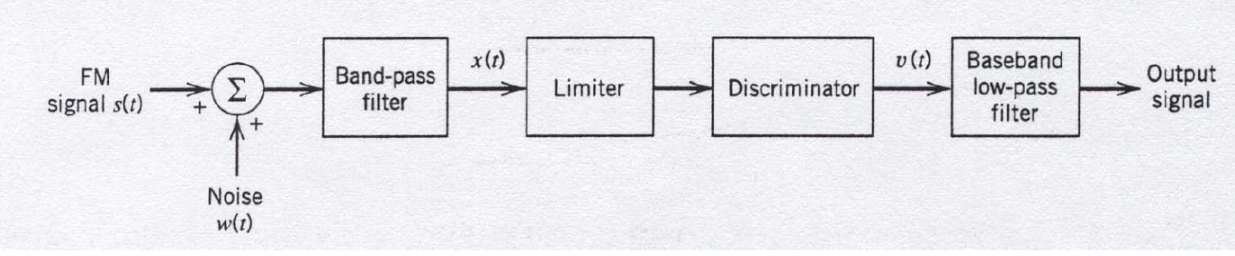
\includegraphics[width=0.9\textwidth]{img/ChaineDemod.png}
    \caption{}
    \label{fig : chaine demod}
\end{figure}

\subsection{Effet du bruit}

Le \textbf{B}ruit \textbf{B}lanc \textbf{G}aussien \textbf{A}dditif d'amplitude $N_0/2$, de porteuse $f_c$ et de bande $B_T$ est :
\begin{align*}
n(t) &= \textcolor{green}{n_I(t)}cos[2\pi f_ct] + \textcolor{red}{n_Q(t)} sin[2\pi f_c t]\\
&= r_n(t) cos[2\pi f_ct + \psi_n(t)]
\end{align*}

Avant d'entrer dans le discriminateur, on a :
$$ r(t) = A_c cos[2\pi f_c t + \phi(t)] + r_n(t) cos[2\pi f_c t + \psi_n(t)]$$

\begin{figure}[H]
    \centering
    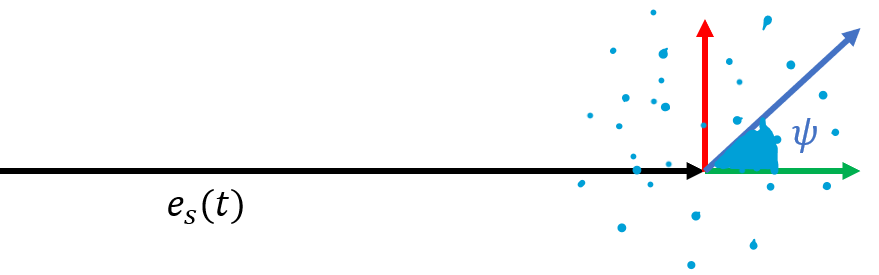
\includegraphics[width=0.5\textwidth]{img/sortieLimiteur.png}
    \caption{}
    \label{fig : chaine demod}
\end{figure}

On remarque que la composante $\textcolor{red}{n_Q(t)}$ aura le plus gros impact sur la phase $\psi$ qui est d'ailleurs une variable aléatoire équitablement distribuée. \\
Il est possible d'exprimer la phase instantanée de ce signal :
$$ \phi_r(t) = \phi(t) + ATN \left\{ \frac{r_n(t) sin[
\overbrace{\psi_n(t) - \phi(t)}^{\mathclap{\text{aussi une équiprobable}}}
]}{A_c+r_n(t)cos[\psi_n(t) - \phi(t)]} \right\} $$
On fait l'hypothèse que l'on a un bon SNR et donc $A_c$ est dominant. On peut affirmer que le numérateur possède les mêmes propriétés statistiques que $\textcolor{red}{n_Q(t)}$.\\
A la sortie du discriminateur, on une phase proportionnelle à $\frac{1}{2\pi}\frac{d\phi_r(t)}{dt}$ :
$$\frac{1}{2\pi}\frac{d\phi_r(t)}{dt} = \underbrace{k_f\ m(t)}_{\text{utile}} + \underbrace{\frac{1}{2\pi A_c}\frac{d\{
\overbrace{
 r_n(t) sin[
  \overbrace{
  \psi_n(t)-\phi(t)]
 }^{\simeq \psi_n(t)} }^{= - n_Q(t)}
 \} }{dt}}_{\text{bruit}}$$
 
Au niveau des densités spectrales, on a brièvement:
\begin{align*}
&\frac{N_0}{2}
&&& 
\rightarrow
\boxed{ \times| H(\omega)|^2 } \rightarrow 
&&&
2N_0 
&&&
\rightarrow 
\times \frac{1}{2}
\left\{
\begin{array}{l}
N_I(\omega)\\
N_Q(\omega)
\end{array}
\right.
\rightarrow 
&&&
N_0
&&&
\rightarrow 
\boxed{\times |j\omega|^2} \rightarrow 
&&& \omega^2\ N_0
\end{align*}

\begin{figure}[H]
    \centering
    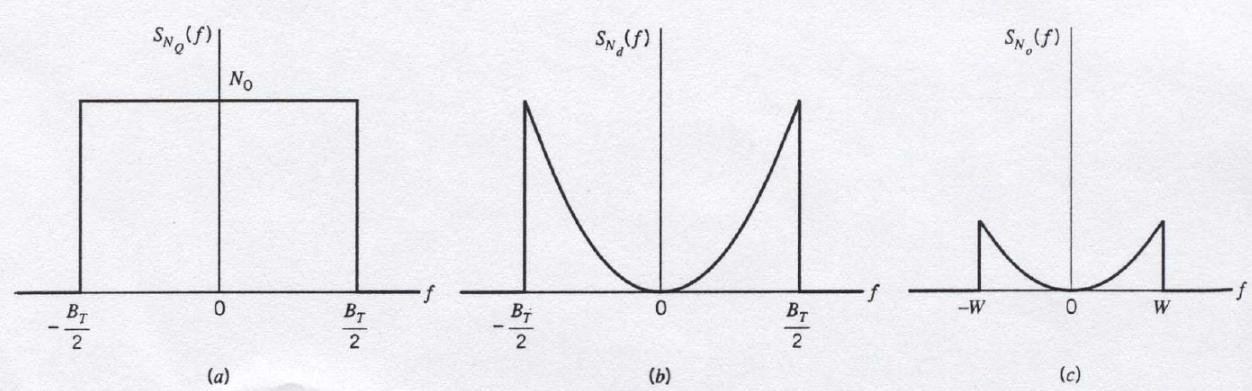
\includegraphics[width=0.8\textwidth]{img/bruit.png}
    \caption{}
\end{figure}
\noindent
On a d'une part le bruit : \begin{align}
n_d(t) &= -\frac{1}{2\pi A_c}\frac{d\{n_Q(t)\}}{dt}\\
N_d(\omega) &= -j\omega N_Q(\omega)/2\pi A_c
\end{align}
et le terme utile de puissance
\begin{equation}
k_f^2 P_m
\end{equation}
On trouve la puissance contenue dans le bruit :
\begin{align*}
\textbf{E}[N_d(\omega)N_d^*(\omega')] &= \frac{-j\omega}{2\pi A_c}\frac{j\omega}{2\pi A_c}\textbf{E}[N_Q(\omega)N_Q^*(\omega')]\\
&= \frac{\omega^2}{2\pi A_c^2}N_0 \delta(\omega - \omega')\\
\gamma_{N_d}(\omega) &= \frac{\omega^2 N_0}{(2\pi A_c)^2} \quad |\omega|/2\pi \leq B_T/2
\end{align*}
On passe ensuite le signal dans un filtre autour du signal modulant de largeur $W$. \\
Les grandeurs de bruit :
\begin{align}
&\text{Puissance de bruit :} &&& \sigma_{n_0}^2 &= \frac{1}{2\pi}\int_{-W}^W \frac{\omega^2 N_0}{(2\pi A_c)^2}d\omega = \frac{2N_0 W^3}{3 A_c^2} \\
&\text{Rapport signal à bruit :}&&&
SNR_0 &= \frac{k_f^2 P_m}{2N_0 W^3/3A_c^2}=\frac{3 A_c^2 k_f^2 P_m}{2N_0 W^3}
\end{align}
\begin{align}
SNR_c &= \frac{A_c^2}{2N_0 W}\\
\text{Gain : } G_m &= \frac{SNR_0}{SNR_c} = \frac{3k_f^2 P_m}{W^2}
\end{align}
Or on a que pour un signal qui n'est pas à simple ton, on a $D=\frac{\Delta f}{W}\propto \frac{k_f P_m^{0.5}}{W}$. On voit donc que si on augmente la bande et donc $B_T$, on augmente $\Delta f$ ce qui va améliorer le gain !\\

On observe aussi que toute les fréquences ne seront pas affectées de la même manière par le bruit. Une solution à cela est de préaccentuer et désaccentuer les signaux pour que l'affectation du bruit soit répartie:
\begin{figure}[H]
    \centering
    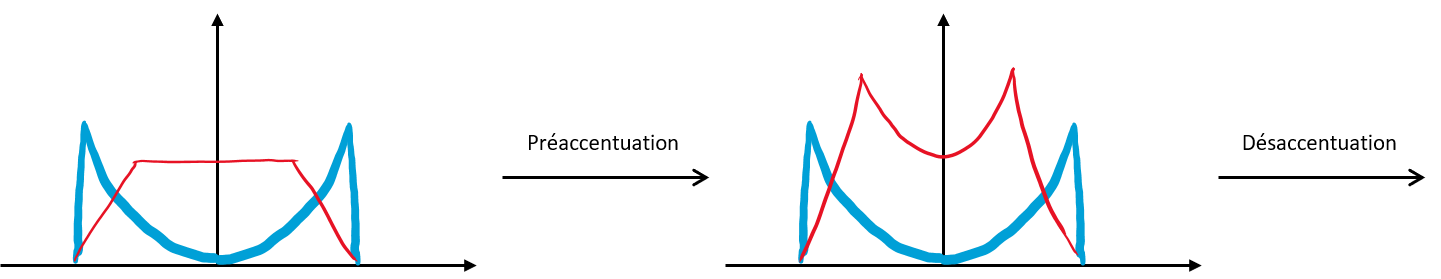
\includegraphics[width=0.8\textwidth]{img/accent.png}
    \caption{}
\end{figure}

\subsubsection{Effet de seuil}

On observe aussi l'effet de seuil pour la démodulation FM. Un valeur typique de seuil est un SNR d'entrée de 10 dB.\\

\textbf{remarque} : La modulation FM sera préférée pour des signaux sujets à de fortes non-linéarités car la phase est assez bien préservée de celles-ci.

\section{Phase Locked Loop PLL}
\begin{figure}[H]
    \centering
    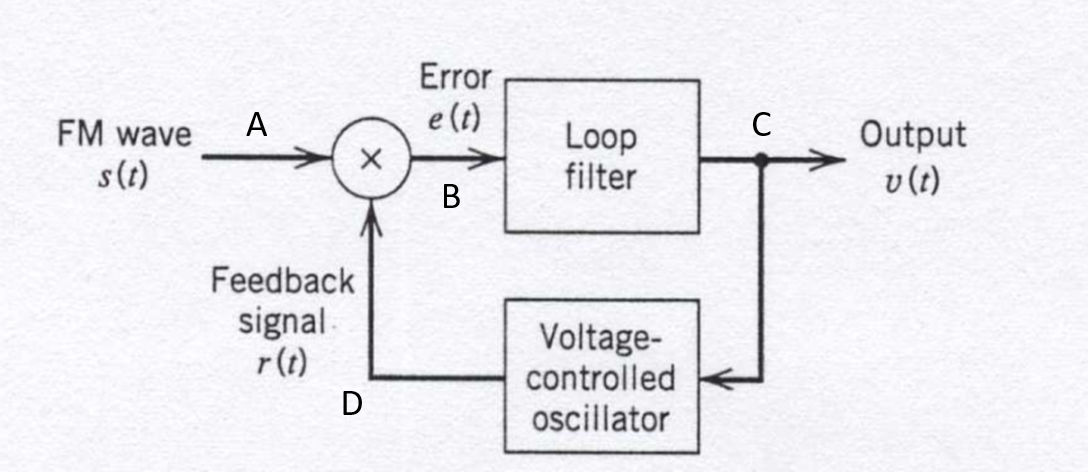
\includegraphics[width=0.5\textwidth]{img/PLL.png}
    \caption{}
\end{figure}
\noindent
En \textbf{A} - on a $s(t) = A_c sin[2\pi f_c t +\phi_1(t)]$ avec $\phi_1(t) = 2\pi k_f \int_0^T m(\tau) d\tau $. \\
\noindent En \textbf{D} - $r(t) = A_v cos[2\pi f_c t + \phi_2(t)]$ où $\phi_2(t) = 2\pi k_v \int_0^t v(\tau) d\tau$.\quad $k_v$ est la sensibilité du VCO\\
\noindent En \textbf{B} - à la sortie du multiplicateur, on filtre le signal pour ne garder que la composante en $e(t) = k_m A_c A_v sin[\phi_1(t) - \phi_2(t)]= k_m A_c A_v sin[\phi_1(t) -2\pi k_v \int_0^t v(\tau) d\tau]$\\
\noindent En \textbf{C} - à la sortie du filtre de boucle on aura :
$$\frac{d\phi_e(t)}{dt}=\frac{d\phi_1(t)}{dt} - 2\pi K_0 \int_{-\infty}^{\infty} sin[\phi_e(t)]h(t-\tau)d\tau$$

\subsubsection*{modèle linéaire}

Lorsque l'erreur de phase est petite, la boucle est dite "accrochée" ou en "phase lock". On peut alors approximer $sin[\phi_e(t)]$ par $\phi_e(t)$:
\begin{figure}[H]
    \centering
    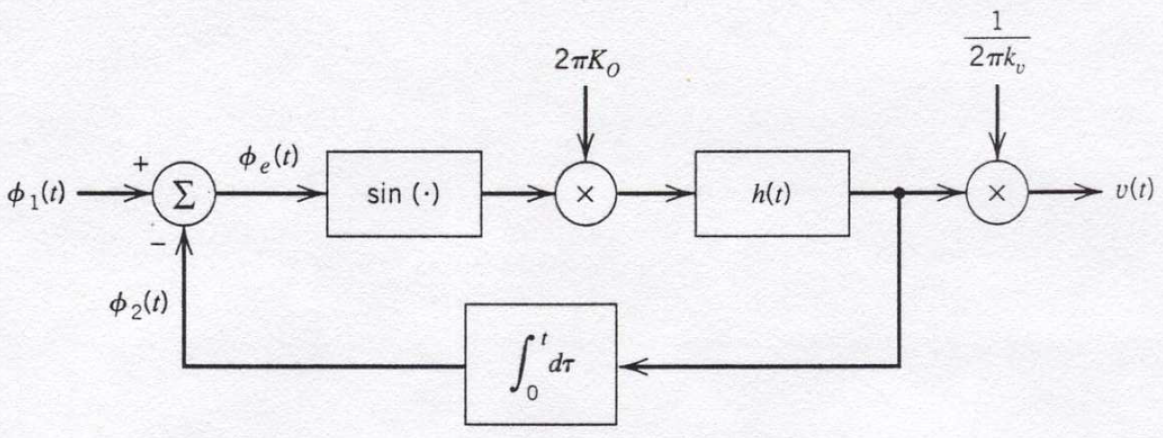
\includegraphics[width=0.5\textwidth]{img/line.png}
    \caption{}
\end{figure}

On trouve alors :
\begin{equation}
\frac{\Phi_2(\omega)}{\Phi_1(\omega)}=\frac{2\pi K_0 H(\omega)}{j\omega + 2\pi K_0 H(\omega)}
\end{equation}
Ce qui montre que les deux phases se suivent bien !

\section{Récepteur superhétérodyne}
contourne la difficulté associée à la construction d'un filtre sélectif et devant pouvoir être déplacé sur l'axe des fréquences. Contenu dans tous les récepteurs radio. Attention aux fréquences images !
\begin{figure}[H]
    \centering
    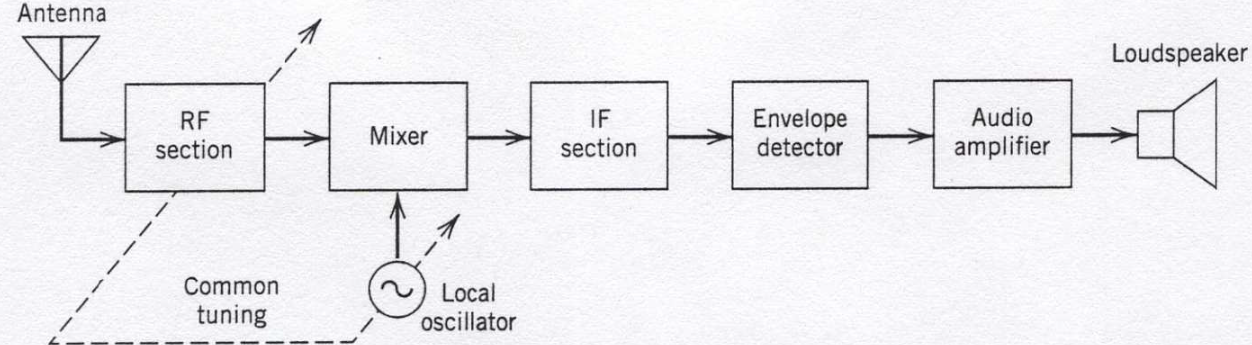
\includegraphics[width=0.6\textwidth]{img/super.png}
    \caption{}
\end{figure}

\part{Transmissions numériques}


\section{Quantification}

La première étape est de passer d'un signal analogique en digital en quantifiant le signal. Cette opération entraîne une perte de précision et est irréversible. 

\begin{figure}[H]
    \centering
    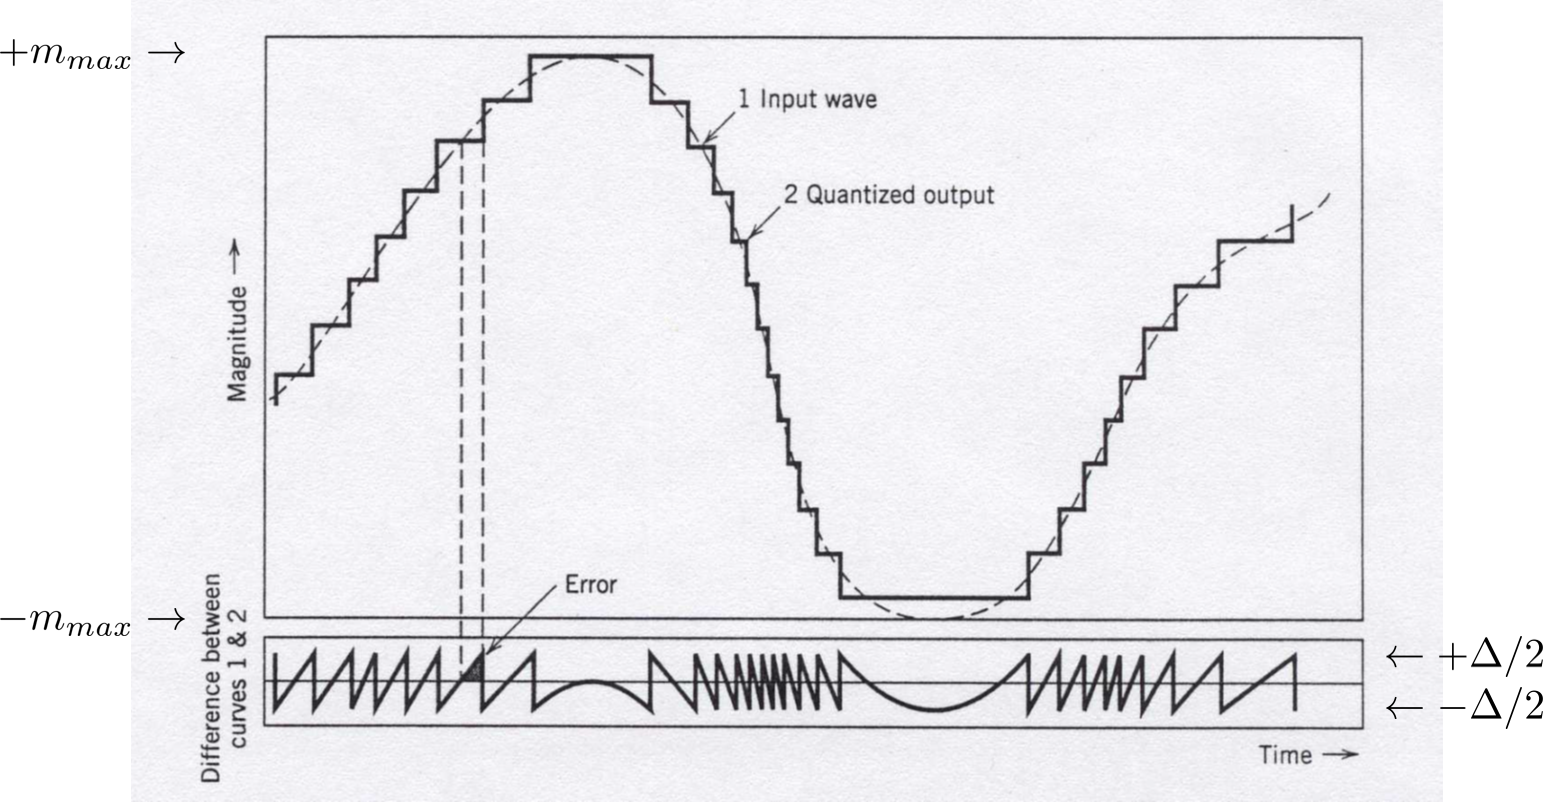
\includegraphics[width=0.7\textwidth]{img/BruitQuantTEX.png}
    \caption{Différence entre signal et signal quantifié appelée bruit de quantification}
\end{figure}

On pourra faire l'hypothèse de considérer la quantification comme un bruit additif au signal de base. Ce bruit aura une densité de probabilité plate, on peut donc en calculer la moyenne et la variance. On aura :
$$
f_Q(q)=
\left\{
\begin{array}{l}
  \frac{1}{\Delta} \quad -\Delta/2 \leq q \leq \Delta/2 \\
  0 \quad \text{sinon}
\end{array}
\right.
$$
\begin{align*}
\Delta &= \frac{2\ m_{max}}{L} &&& L&=2^R &&& \sigma^2_Q &= \mathbf{E}[Q^2]=\frac{\Delta^2}{12}
\end{align*}
Avec $R$ le nombre de bits par échantillons. On aura donc : $\sigma^2_Q = \frac{1}{3}m^2_{max}2^{-2R}$\\
Le SNR est donné par :
\begin{align*}
SNR_o &= \frac{P}{\sigma^2_Q}=\left( \frac{3P}{m^2_{max}} \right) 2^{2R}
\end{align*}
On remarque donc que l'on peut améliorer le SNR exponentiellement en consacrant plus de bande passante car cela va de paire avec un accroissement de R.\\

\begin{figure}[H]
    \centering
    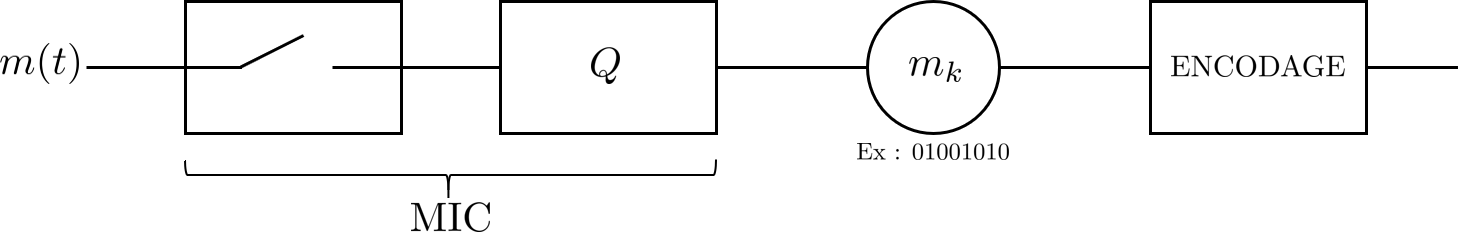
\includegraphics[width=0.7\textwidth]{img/MIC.png}
    \caption{\textbf{M}odulation par \textbf{I}mpulsions \textbf{C}odées ou \textbf{PCM}}
\end{figure}

\section{Compression}

Le signal entrant est volontairement échantillonné à un rythme supérieur au rythme de Shannon. Ceci a pour effet de rendre les échantillons successifs fortement corrélés. Il est donc possible de réduire le débit en comprimant le signal au strict minimum pour pouvoir reconstituer le signal original à la démodulation.

\subsection{Modulation delta}

\begin{figure}[H]
    \centering
    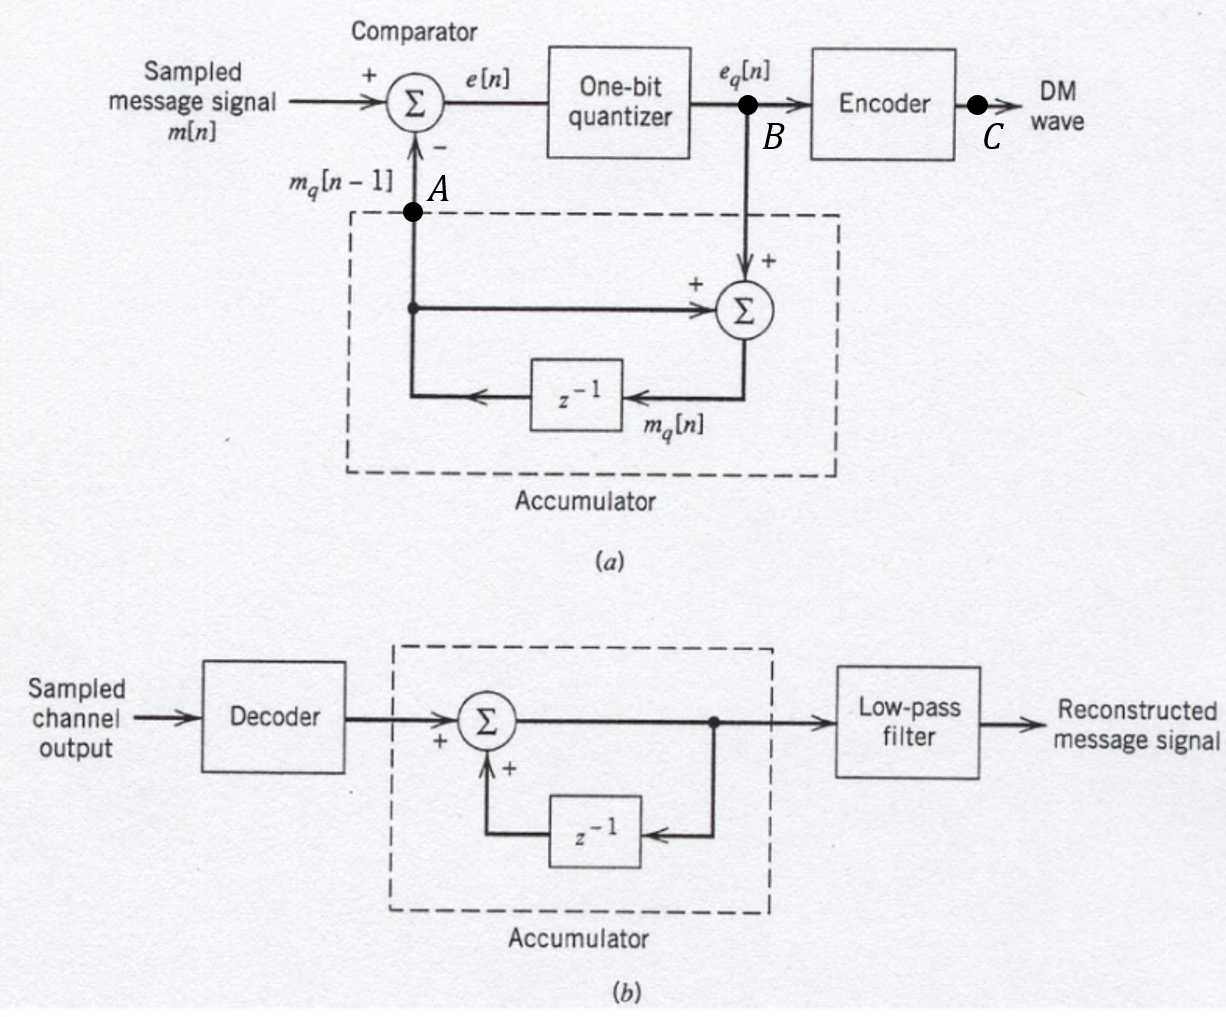
\includegraphics[width=0.7\textwidth]{img/delta.png}
    \caption{Modulation delta}
\end{figure}
\begin{enumerate}[label=(\Alph*)]
\item prédiction proposée = signal précédent DÉCODÉ car seul l'encodeur a les valeurs précédentes originales !
\item signe de l'erreur commise 
\item $\pm \delta$
\end{enumerate}

Il se peut que l'on ait des oscillation entre + et - , 1 et 0. Ceci sera appelé un bruit granulaire. Il est dû au fait qu'on a un pas $\delta$ constant. On voudra à l'avenir pouvoir adapter ce pas.

\subsection{Modulation delta adaptative}
\begin{itemize}
\item si erreurs successives sont de types >< on réduit le pas
\item sinon le quantificateur est susceptible d'être en surcharge : judicieux d'augmenter le pas.
\end{itemize}

\subsection{Codage prédictif}
Idée : \\
Si on a un signal $m[n]$ et sa prédiction $\hat{m}[n]=m_q[n-1]$ codés sur 8 bits, on aura une erreur $e[n]$ ayant une valeur comprise entre [-255 , 255]. On passe donc de 8 à 9 bits à l'émission. On aimerait donc attribuer à des échantillons plus courants, des symboles moins longs pour réduire le débit. Cela s'appelle faire du \textbf{V}ariable \textbf{L}enght \textbf{C}oding. C'est l'idée implémentée dans le Morse.

\begin{figure}[H]
    \centering
    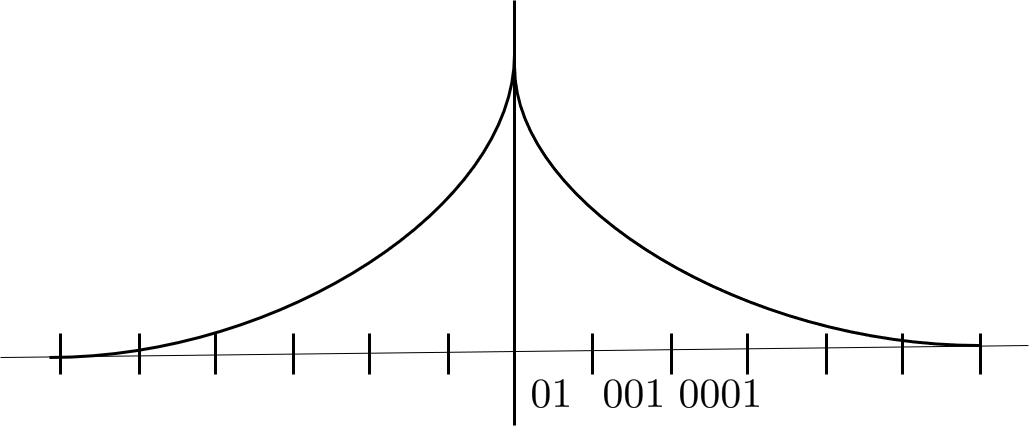
\includegraphics[width=0.4\textwidth]{img/VLC.png}
    \caption{Densité de probabilité de $e[n]$}
\end{figure}

Il sera cependant nécessaire que les codes ne soient pas les préfixes des autres car il est maintenant primordial de pouvoir délimiter chaque paquet de longueur variable. 

\subsection{Codage par transformée}

Plutôt que de quantifier les échantillons eux-mêmes, on applique aux blocs (par exemple de 8 ou 16 bits) une transformée bien choisie. Une des motivations est qu'avec les transformées utilisées, il est possible d'accorder une signification spectrale aux coefficients transformés. Comme la sensibilité de l’œil ou de l'oreille n'est pas a même à toutes les fréquences, on peut utiliser des pas de quantification différents pour différents coefficients obtenus.\\
Soit $\bar{X}$ un bloc de N échantillons auquel on applique une transformée : $ \underline{Y} = \doubleunderline{A}\ \underline{X} $\\
La matrice de covariance est donnée par : $\doubleunderline{R}_Y = \doubleunderline{A}\ \doubleunderline{R}_X\ \doubleunderline{A}^T$\\
Si la matrice de covariance de départ admet une décomposition en vecteurs et valeurs propres :

\begin{align*}
\doubleunderline{R}_X &= \doubleunderline{M}_X\ \doubleunderline{\Lambda}_X\ \doubleunderline{M}_X^T \\
\doubleunderline{R}_Y &= \doubleunderline{A}\  \doubleunderline{M}_X\ \doubleunderline{\Lambda}_X\ \doubleunderline{M}_X^T\ \doubleunderline{A}^T
\end{align*}

Le choix $\doubleunderline{A} = \doubleunderline{M}_X^{-1}$ permet de rendre $\doubleunderline{R}_Y$ diagonale, c'est à dire de décorréler les composantes de ce vecteur. 

\subsubsection*{La télévision numérique}
L'échantillonnage en horizontale revient à découper chaque ligne en picture-elements (pixels). La bande passante occupé par la luminance $Y$ est de l'ordre de 13.5 MHz et de l'ordre de 6.75 MHz pour les 2 signaux de chrominance. Soit un total de 27 millions d'échantillons par seconde. Si l'on quantifie sur 8 bits donc 256 niveaux, on aura $27 \times 10^6  \times 8 = 216$ Mbits/s !!! \\
Si on ne garde que la partie active des lignes, on peut gagner 25\%. D'autres techniques prédictives sont utilisées et du codage par transformée sont utilisés pour réduire au minimum le débit.

\begin{figure}[H]
    \centering
    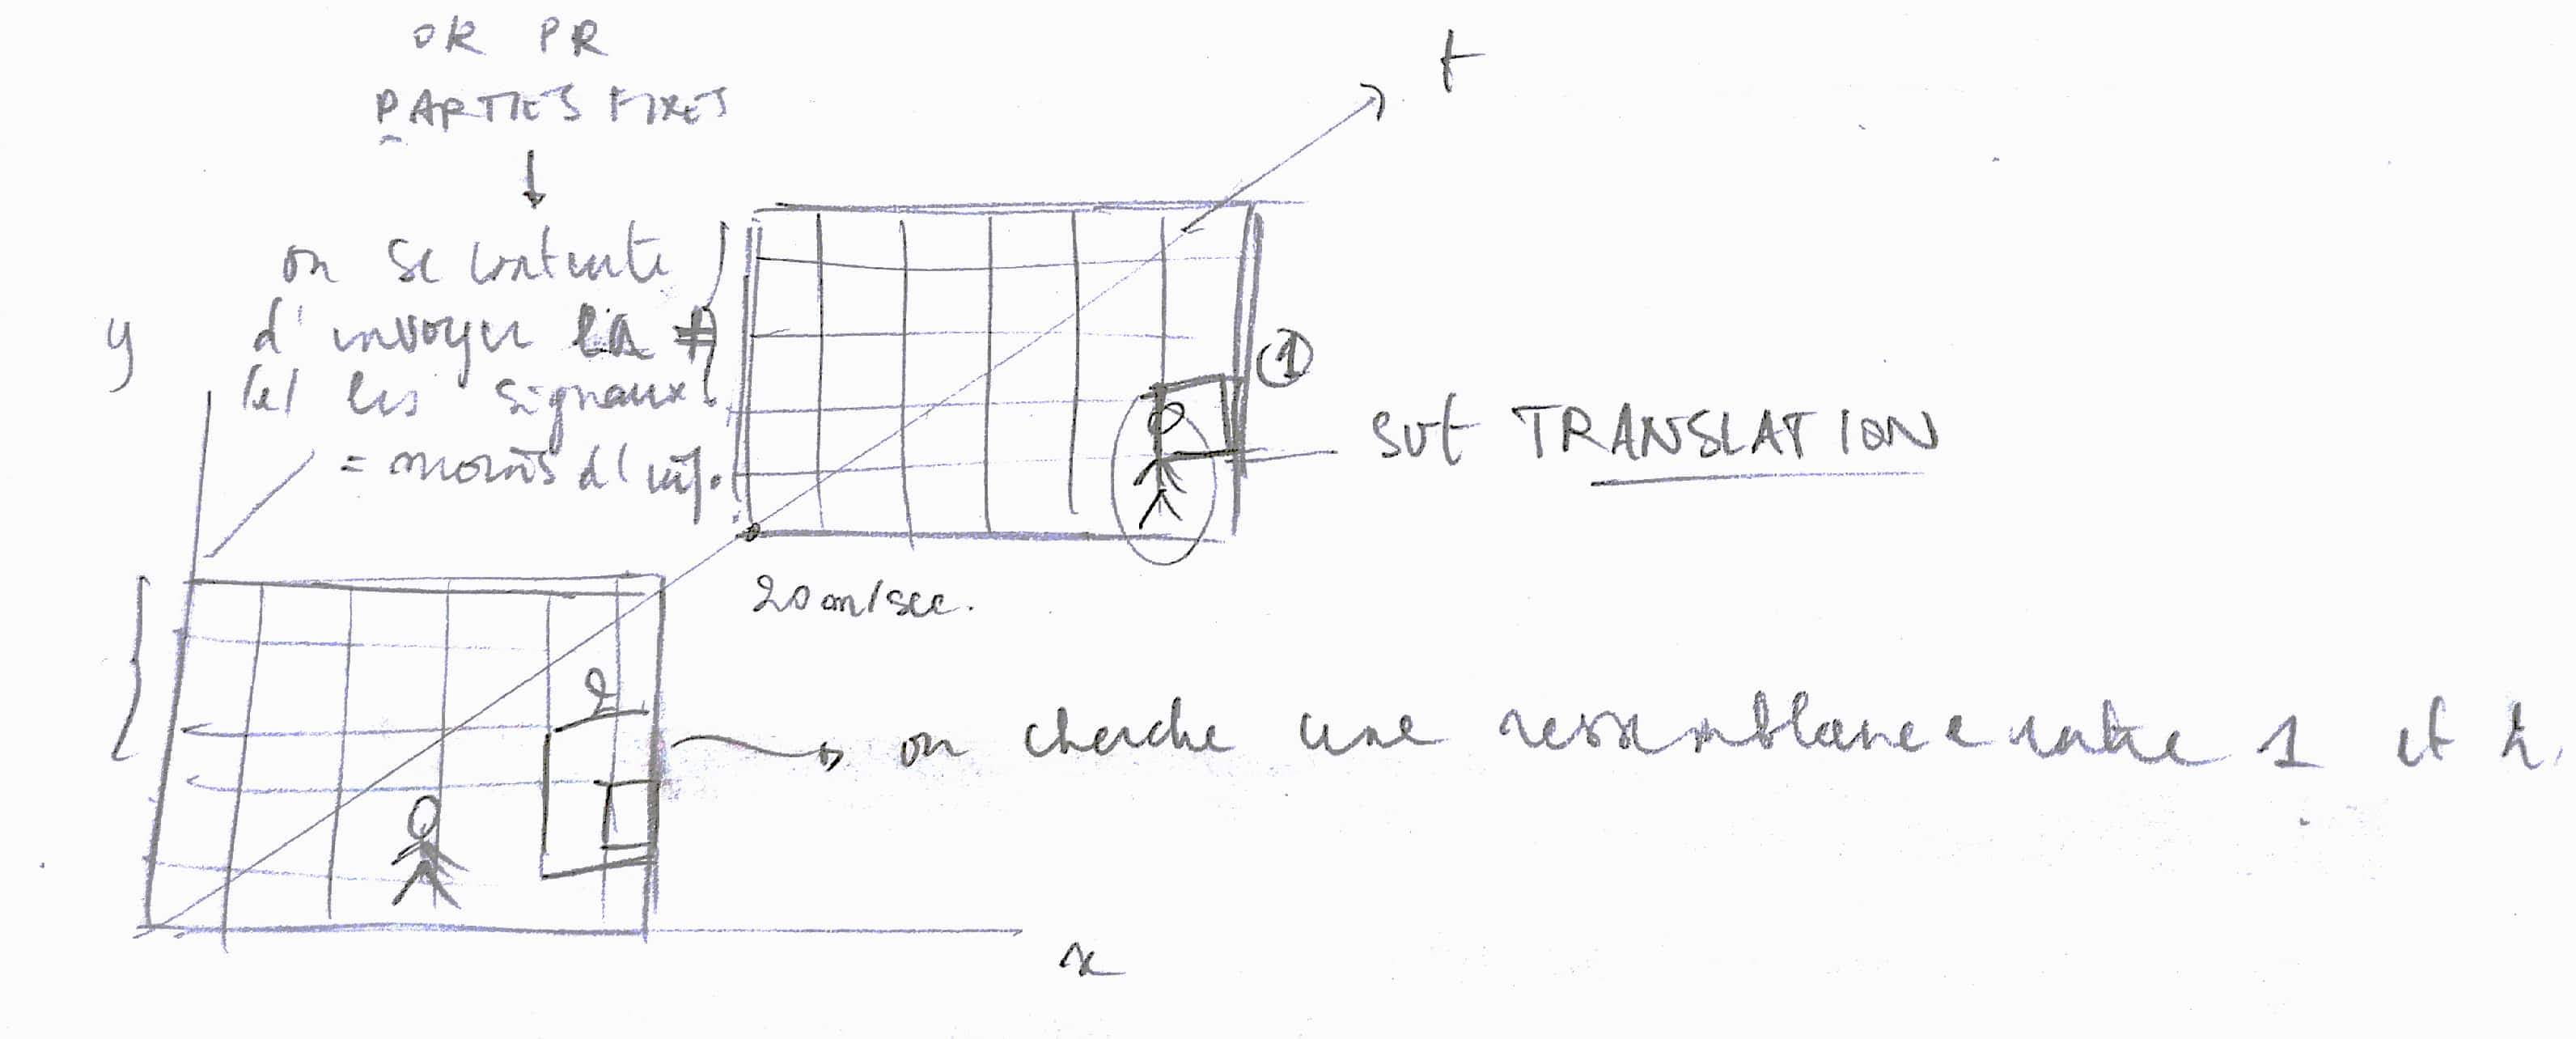
\includegraphics[width=0.8\textwidth]{img/TVnum.jpg}
    \caption{}
\end{figure}

\section{Transmission en bande de base}

\subsection{Codes en ligne}

Utilisés pour pouvoir se superposer aux signaux analogiques du son [20 20k] Hz. Évolution des codes en ligne :
\begin{enumerate}
\item \textit{unipolaire NRZ} ou non return to zero
\item \textit{NRZ polaire}
\item \textit{RZ unipolaire}
\item \textit{RZ bipolaire}
\item \textit{Manchester}
\end{enumerate}
Le cahier des charges à remplir était de ne pas empiéter sur la bande de base des signaux sonores et aussi de pouvoir assurer une bonne distinction entre les symboles. C'est pourquoi il a fallu se débarrasser de toute composante DC, éviter les signaux qui aient une densité spectrale empiétant sur les basses fréquence et éviter les longs trains de symboles.

\begin{figure}[H]
    \centering
    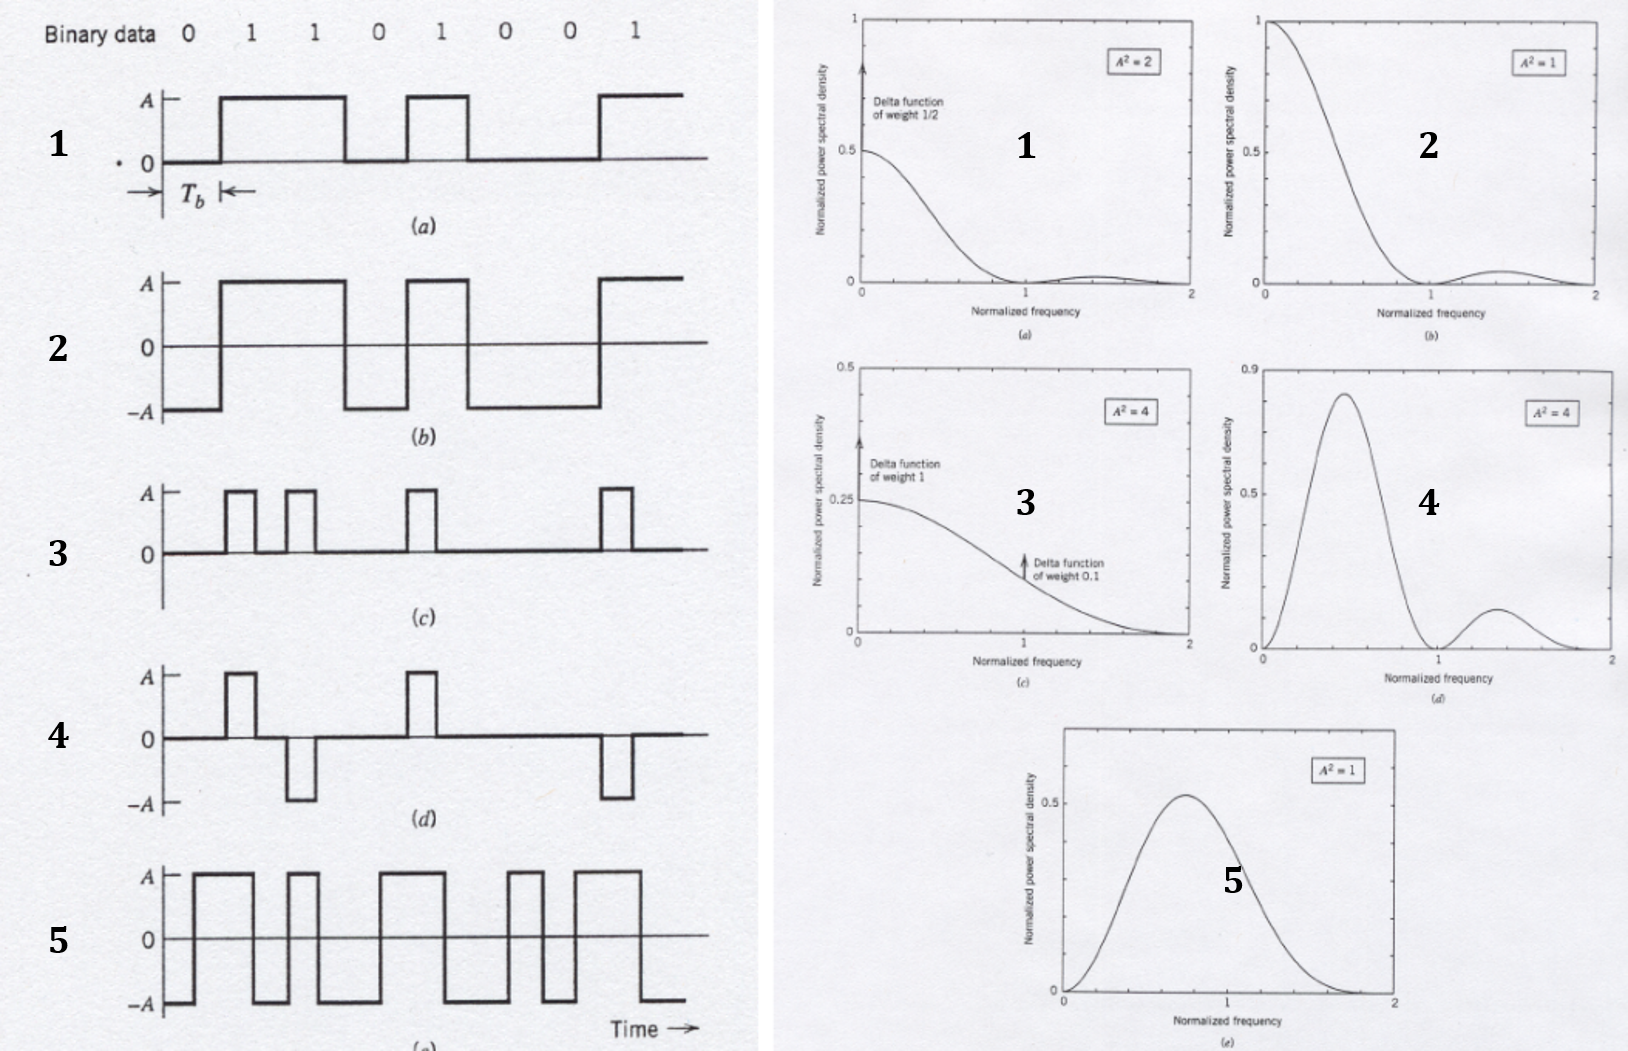
\includegraphics[width=\textwidth]{img/lignes.png}
    \caption{codes en lignes : temporel et densités spectales}
    \label{ligne}
\end{figure}

L'unité de transmission de symbole par seconde est le BAUD. Sur la figure \ref{ligne}, on aura un débit de $\frac{1}{T_b} [BAUD]$

%\newpage

\subsection{Maximisation rapport signal à bruit}
Problème :\\

\begin{figure}[H]
    \centering
    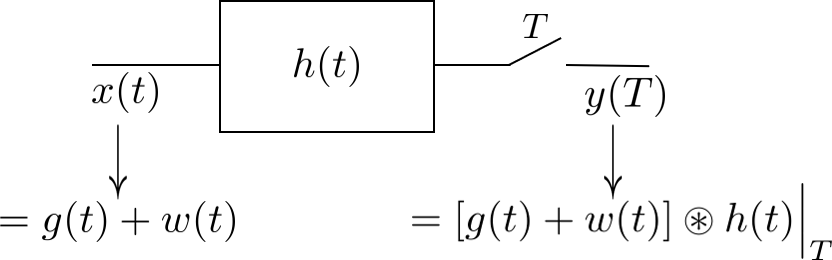
\includegraphics[width=0.5\textwidth]{img/prob.png}
    \caption{}
\end{figure}

Le rapport signal à bruit en temporel :

$$ SNR = \dfrac{\left| \frac{1}{2\pi} \int G(\omega)\ H(\omega)\ e^{j\omega T} d\omega \right|}{\frac{N_0}{4\pi}  \int \left| H(\omega) \right|^2 d\omega} $$

On sait de part l'inégalité de Schwarz, que le membre de gauche de l'inégalité suivante : 

$$ \left| \int_{-\infty}^{\infty} \phi_1(x) \phi_2(x) dx \right|^2 \leq \int_{-\infty}^{\infty} \left| \phi_1(x) \right|^2 dx\ \int_{-\infty}^{\infty} \left| \phi_2(x) \right|^2 d$$

est maximisé pour : \quad $\phi_1(x) = k \phi_2^*(x)$ \\ 
\indent Si on remplace $\phi_1(x)=H(\omega)$ et $\phi_2(x) = G(\omega)\ e^{j\omega T}$ on requiert :
\begin{align*}
H(\omega)&=k\ G^*(\omega) e^{-j\omega T}  &&& h(t) &= k\ g^*(T-t)
\end{align*}

Le filtre optimal a donc une réponse impulsionnelle qui est, à un facteur $k$ près, la version retournée et décalée de la forme d'onde utilisée en émission. On appelle ce filtre un \textbf{filtre adapté}.\\
Le rapport signal à bruit devient :
\begin{align*}
SNR &=  \dfrac{\left| \frac{1}{2\pi} \int \cancel{k}\ \left| G(\omega)\right|^2 \  d\omega \right|^2}{\frac{N_0}{4\pi} \int  \cancel{k^2} \left| G(\omega) \right|^2 d\omega} = \dfrac{\frac{1}{2\pi} \int \ \left| G(\omega)\right|^2 \  d\omega}{\frac{N_0}{2}} \\
&= \frac{2 \mathcal{E}_g}{N_0} = \text{SNR maximal auquel on peut prétendre}
\end{align*}
 
L'action opérée par le filtre adapté est équivalente à une corrélation du signal reçu $x(t)$ avec le signal utile que l'on s'attend à recevoir $g(t)$.\\
\underline{NB} : corréler avec $g(t)$ = convoluer avec $g(-t)$\\

\subsection{BER}

\subsection*{Signaux en transmission NRZ}


Si on s'intéresse à une transmission NRZ avec un signal reçu dans l'intervalle de durée $T_b$ :

\begin{align*}
x(t)	&=
\left\{
\begin{array}{l}
  +A+w(t) \quad \text{Pour l'envoi d'un 1} \\
  -A+w(t) \quad \text{Pour l'envoi d'un 0}
\end{array}
\right.
&&&
g(t) &= \pm rect_{T_b}(t)
\end{align*}

\begin{align*}
y(t) &= \int_{-\infty}^{\infty} x(t) rect_{T_b}(t) dt&&&  &\stackrel{\text{POUR UNE FENÊTRE}}{=} &&& \frac{1}{T_b}\int_0^{T_b} x(t) dt\\
&= \frac{1}{T_b}\int_0^{T_b} (A+\omega(t)) dt = A+\underbrace{\frac{1}{T_b}\int_0^{T_b} w(t) dt}_{\nu}
\end{align*}

\begin{figure}[H]
    \centering
    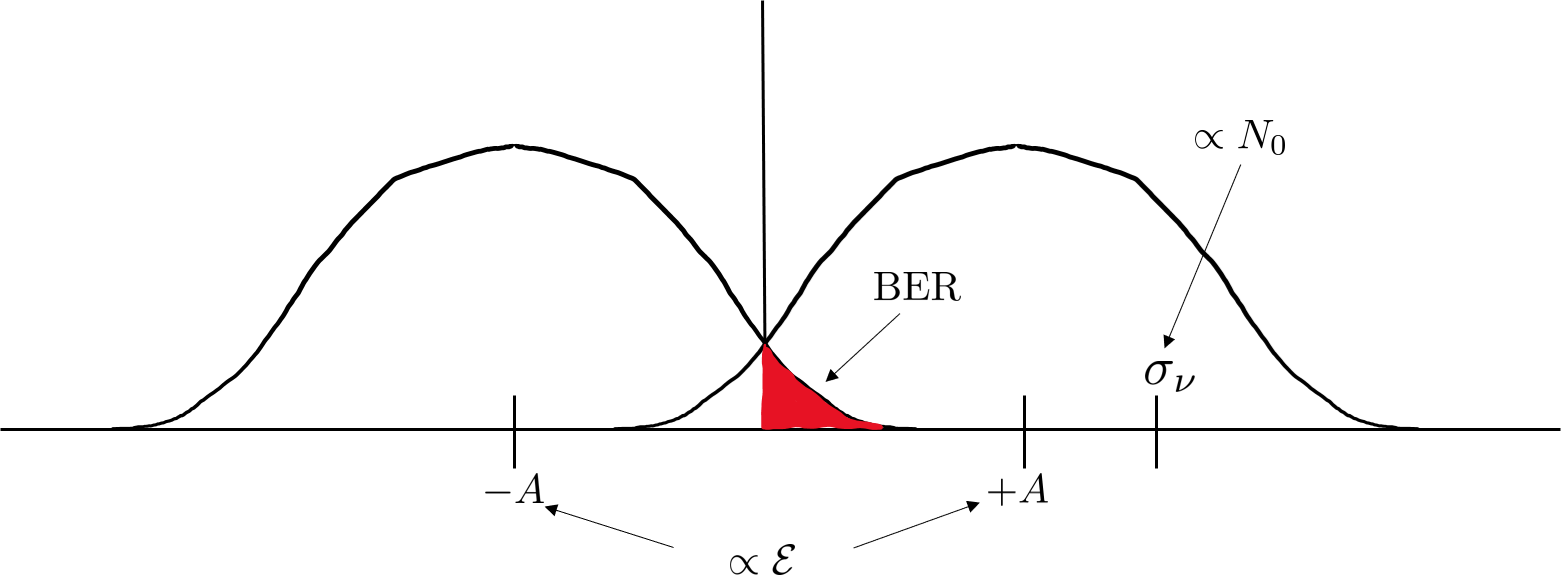
\includegraphics[width=0.6\textwidth]{img/BER.png}
    \caption{}
\end{figure}

On aura :
\begin{align*}
\sigma^2_{\nu} = \mathbf{E}[\nu^2] &= \mathbf{E}\left[\frac{1}{T_b^2} \int_0^{T_b} w(t) dt  \int_0^{T_b} w(t') dt' \right]\\
&= \frac{1}{T_b^2} \int_0^{T_b} dt  \int_0^{T_b} dt' \mathbf{E}[w(t) w(t')]\\
&= \frac{1}{T_b^2} \int_0^{T_b} dt  \int_0^{T_b} dt' \frac{N_0}{2} \delta(t-t')\\
&= \frac{N_0}{2T_b}
\end{align*}

Le seuil de décision est calculé de la sorte :
$$\int x(t) s_0(t) dt \lessgtr \int x(t) s_1(t) dt \ \leftrightarrow \ \int x(t) [s_0(t)-s_1(t)]dt \lessgtr 0$$



La probabilité de faire une erreur est donnée par :

$$ p_e = p[0|1]p_1 + p[1|0]p_0 $$

$p_1$ et $p_0$ sont les probabilités d'avoir un 1 ou un 0. 

\subsubsection*{Envoi du 0}

La densité de probabilité de $Y$ conditionnellement à l'envoi du 0 est une gaussienne
\footnote{ $ f(x) = \dfrac{1}{\sigma \sqrt{2\pi}}\ exp^{-\frac{1}{2}\left( \frac{x-\mu}{\sigma} \right)^2}$}
 de moyenne $-A$ et de variance $\frac{N_0}{2T_b}$ :
$$ T_{Y|0}(y|0) = \dfrac{1}{\sqrt{(\pi N_0/T_b)}} exp \left[ -\dfrac{(y+A)^2}{N_0/T_b} \right] $$

Si le seuil de décision est fixé à $\lambda$, on aura une erreur lorsque $Y \geq \lambda$ ou $Z = \frac{Y-m_y}{\sigma_{Y|0}} \geq \frac{\lambda - m_y}{\sigma_{Y|0}}$

\begin{align*}
p[1|0] &= \int_{\lambda}^{\infty} \dfrac{1}{\sqrt{(\pi N_0/T_b)}} exp \left[ -\dfrac{(y+A)^2}{N_0/T_b} \right] dy \\
&= \int_{\frac{\lambda +A}{\sqrt{N_0/2T_b}}}^{\infty} \dfrac{1}{\sqrt{2\pi}} exp \left[ -\dfrac{z^2}{2} \right] dz 
&&& \boxed{erfc(u) = \int_u^{\infty} \frac{2}{\sqrt{\pi}} exp (-x^2) dx  } \\
&= 0.5 \ erfc \left( \dfrac{A+\lambda}{\sqrt{N_0/T_b}} \right)
\end{align*}

On notera en passant la relation :

$$ P(Y>u) = \frac{1}{2}erfc \left( \frac{u}{\sqrt{2}}\right) \quad \text{pour} \quad Y\sim \mathcal{N}(0,1)$$

\subsubsection*{Envoi du 1}

La densité de probabilité de $Y$ conditionnellement à l'envoi du 1 est une gaussienne de moyenne $+A$ et de variance $\frac{N_0}{2T_b}$ :
$$ T_{Y|1}(y|1) = \dfrac{1}{\sqrt{(\pi N_0/T_b)}} exp \left[ -\dfrac{(y-A)^2}{N_0/T_b} \right] $$

Si le seuil de décision est fixé à $\lambda$, on aura une erreur lorsque $Y \leq \lambda$ ou $Z = \frac{Y-m_Y}{\sigma_{Y|1}} \leq \frac{\lambda - m_y}{\sigma_{Y|1}}$

\begin{align*}
p[0|1] &= \int_{-\infty}^{\lambda} \dfrac{1}{\sqrt{(\pi N_0/T_b)}} exp \left[ -\dfrac{(y-A)^2}{N_0/T_b} \right] dy \\
&= \int_{-\infty}^{\frac{\lambda -A}{\sqrt{N_0/2T_b}}} \dfrac{1}{\sqrt{2\pi}} exp \left[ -\dfrac{z^2}{2} \right] dz\\
&= 0.5 \ erfc \left( \dfrac{A-\lambda}{\sqrt{N_0/T_b}} \right)
\end{align*}

Pour des signaux équiprobables, on aura :
\begin{align*}
\lambda &=0 &&& \mathcal{E}_b&=A^2T_b
\end{align*}

\begin{align*}
p_e &= p[0|1]\frac{1}{2} + p[1|0]\frac{1}{2}\\
&= 0.5 \ erfc\left(\frac{A}{\sqrt{N_0/T_b}} \right)\\
&= 0.5 \ erfc\left( \sqrt{\frac{\mathcal{E}_b}{N_0}} \right)
\end{align*}

\begin{figure}[H]
    \centering
    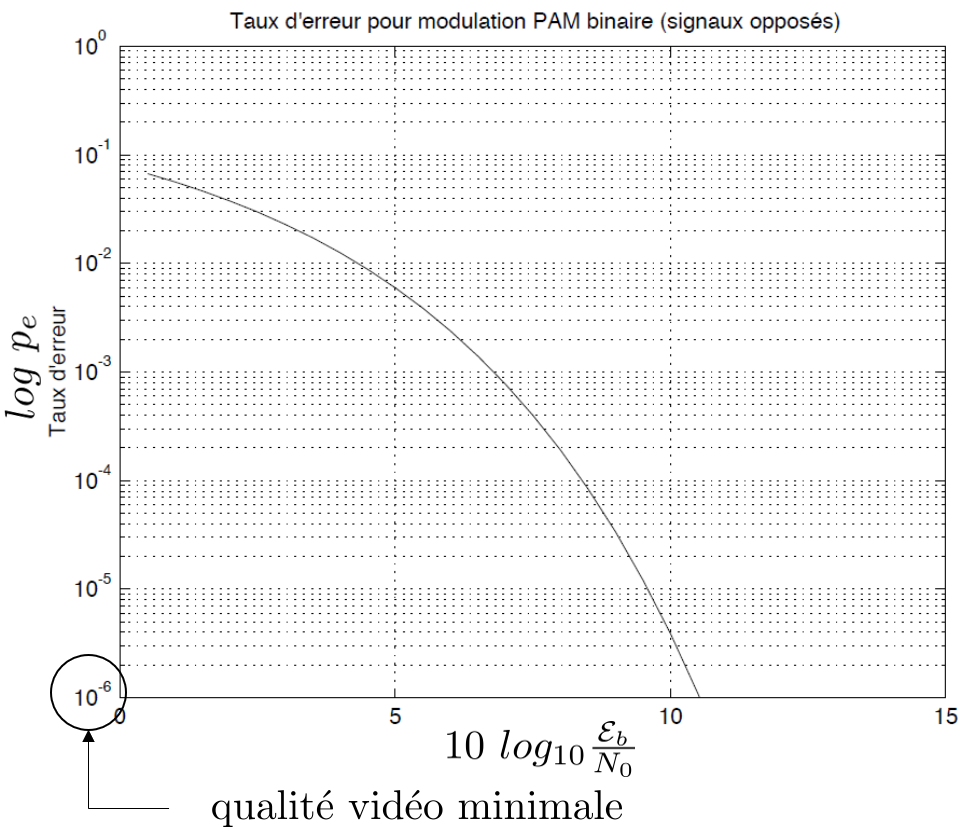
\includegraphics[width=0.6\textwidth]{img/Pe.png}
    \caption{Log de la $p_e$ \textbf{pour des signaux opposés}}

\end{figure}

\subsection*{Signaux de corrélation quelconque}
Si on travaille avec l'envoi de 0 par $s_0(t)$ d'énergie $\mathcal{E}_0$ et l'envoi de 1 par $s_1(t)$ d'énergie $\mathcal{E}_1$, le seuil de décision sera calculé en comparant cette fois-ci les distances euclidiennes :
\begin{align*}
\int (x(t) - s_0(t))^2 dt &\lessgtr \int (x(t) - s_1(t))^2 dt \\
\xcancel{\int x^2(t)\ dt} - 2\int x(t) s_0(t)\ dt + \int s_0(t)^2\ dt &\lessgtr \xcancel{\int x^2(t)\ dt} - 2\int x(t) s_1(t)\ dt + \int s_1(t)^2\ dt \\
-2\ \int x(t) [ s_0(t) - s_1(t) ]\ dt &\lessgtr \mathcal{E}_1 - \mathcal{E}_0
\end{align*}

Le filtre adapté de corrélation/produit scalaire/projection vu précédement est bien lorsque les deux signaux sont de même énergie (on retombe ici sur le même résultat). Si ce n'est pas le cas, on préfèrera comparer les distances euclidiennes. 

\begin{align*}
Y_0 &= \int_{-\infty}^{\infty} x(t) s_0(t) dt 	&&& &                        &&& Y&=Y_0 - Y_1 \\
Y_1 &= \int_{-\infty}^{\infty} x(t) s_1(t) dt &&& &\text{on décide} &&& &0 \quad si \quad Y_0 \geq Y_1\ ou\  Y\geq 0 \\
      &                                                       &&&  &                        &&& &1\quad  sinon 
\end{align*}

Imaginons que $s_0(t)$ ait été envoyé :

\begin{align*}
Y_0 &=  \int_{-\infty}^{\infty} s_0(t)\ s_0(t)\ dt +  \int_{-\infty}^{\infty} w(t)\ s_0(t) \ dt =\mathcal{E}_0 + \nu_0 \\
Y_1 &=  \int_{-\infty}^{\infty} s_0(t)\ s_1(t)\ dt +  \int_{-\infty}^{\infty} w(t)\ s_1(t) \ dt =C_{01} + \nu_1 \\
Y    &=  \int_{-\infty}^{\infty} s_0(t)\ [s_0(t)-s_1(t)]\ dt +  \int_{-\infty}^{\infty} w(t)\ [s_0(t)-s_1(t)] \ dt =\mathcal{E}_0 -C_{01}+ \nu_0 - \nu_1\\
\end{align*}
avec 
$$ C_{01} = \int_{-\infty}^{\infty} s_0(t)\ s_1(t)\ dt = \rho\ \mathcal{E} \neq covariance $$

Notre variable de décision est donc une gaussienne (normale)
\begin{itemize}
\item
de moyenne : $$\mu = \mathcal{E}_0 -C_{01}$$
\item
de variance ($\neq \ \sum$ variances car signaux non indépendant on a une corrélation) : 
\begin{align*}
\sigma^2 = \mathbf{E}[(\nu_0 - \nu_1)^2]
&= \mathbf{E}\left[ \int_{-\infty}^{\infty} w(t)[s_0(t) - s_1(t)]\ dt \ \int_{-\infty}^{\infty} w(t')[s_0(t') - s_1(t')]\ dt' \right] \\
&= \int_{-\infty}^{\infty} \ \int_{-\infty}^{\infty} [s_0(t) - s_1(t)][s_0(t') - s_1(t')]\mathbf{E}[w(t)w(t')]\ dt\ dt' \\
&= \int_{-\infty}^{\infty} \ \int_{-\infty}^{\infty} [s_0(t) - s_1(t)][s_0(t') - s_1(t')]\frac{N_0}{2}\delta(t-t')\ dt\ dt' \\
&= \frac{N_0}{2} \int_{-\infty}^{\infty}  [s_0(t) - s_1(t)]^2\ dt = \frac{N_0}{2}[ \mathcal{E}_0 + \mathcal{E}_1 - 2 C_{01}]
\end{align*}
\item[]
Si $\mathcal{E}_0 = \mathcal{E}_1 = \mathcal{E}$ et en définissant $\rho \stackrel{\text{$\Delta$}}{=} C_{01}/\mathcal{E}$
\begin{align*}
\mu &= \mathcal{E}(1-\rho) \\
\sigma^2 &=  \mathbf{E}[(\nu_0 - \nu_1)^2] = N_0(\mathcal{E} - C_{01}) = N_0 \mathcal{E}(1-\rho)
\end{align*}
\end{itemize}

\begin{align*}
p_e &= p[s_1|s_0]\frac{1}{2} + p[s_0|s_1]\frac{1}{2}\\
&= 0.5 \ erfc\left( \frac{\mu}{\sqrt{2}\ \sigma} \right) \\
&= 0.5\ erfc \underbrace{ \left(  \sqrt{ \frac{\mathcal{E}(1-\rho)}{2N_0} }\right) }_{\text{terme à maximiser}} 
\end{align*}

On remarque qu'on aura un BER plus faible si on utilise des signaux \underline{opposés} ($\rho = -1$) que si on utilise des signaux \underline{orthogonaux} ($\rho = 0$).

\subsection{Interférence entre symboles}

\begin{figure}[H]
    \centering
    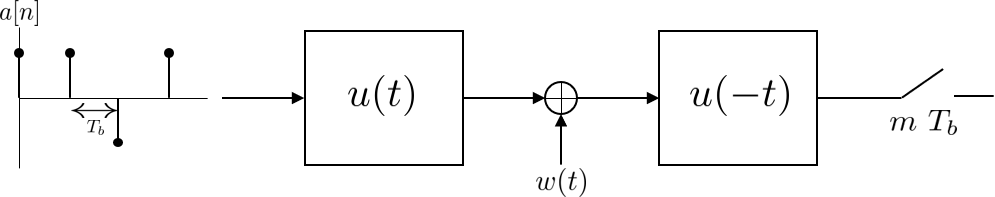
\includegraphics[width=0.8\textwidth]{img/Nyquist.png}
    \caption{}
\end{figure}

Les symboles sont convertis dans le domaine temporel via les filtres $u(t)$. 
Nous avons :
\begin{align*}
r(t) &= \sum_{n=-\infty}^{\infty} a[n]\ u(t-nT_b)+w(t) \\
y[m] &= \int r(t)\ u(t-mT_b)\ dt \\
	&=  \sum_{n=-\infty}^{\infty} a[n] \int u(t-nT_b)\ u(t-mT_b)\ dt + \int w(t) u(t-nT_b)\ dt \\
	&=  \sum_{n=-\infty}^{\infty} a[n] C_a[(m-n)T_b] + \nu[m] \\
\intertext{Pour éviter l' ISI, il est nécessaire que le signal reçu échantillonné en $m\ T_b$ ne soit dépendant que de $n\ T_b$. C'est pourquoi nous imposons l'égalité $n=m$ avec $\delta[m-n]$.}\\
C_a[(m-n)T_b] &= \delta[m-n] \\
C_a[n\ T_b] &= \delta[n] \\
&= \int u(t-nT_b)\ u(t)\ dt \qquad \text{convolution , \st{retournement} , échantillonné $\rightarrow$ périodisé}\\
\textbf{Nyquist} &\rightarrow \frac{1}{T_b} \sum_{k=-\infty}^{\infty} \left| U \left( \omega	- \frac{2\pi k}{T_b}\right) \right|^2 = 1
\end{align*}
\vspace{-4ex}


\begin{figure}[H]
    \centering
    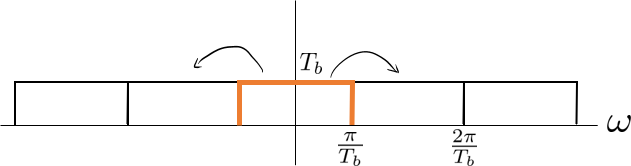
\includegraphics[width=0.5\textwidth]{img/perio.png}
    \caption{}
\end{figure}

Ceci constitue donc la condition à remplir pour éviter d'avoir de l'interférence entre symboles !\\

$\rightarrow$ On est pas capable de faire des transmissions numériques à hauteur de un symbole toutes les $T_b$ secondes \textbf{sans ISI} si on ne dispose pas d'une bande de fréquences de longueur $\frac{1}{T_b}$. \\

En pratique on est pas capables de fabriquer des filtres à pente infinie comme celui ci-dessus. Pour toujours satisfaire à la condition de remplir toutes les plages de fréquence en échantillonnant, on prendra des filtres à flanc de Nyquist, dont les transformées inverses sont des ``raised cosine''. On aura donc un ``roll-off factor'' $\alpha$ qui sera représentatif de l'excès en largeur de bande.

\begin{figure}[H]
    \centering
    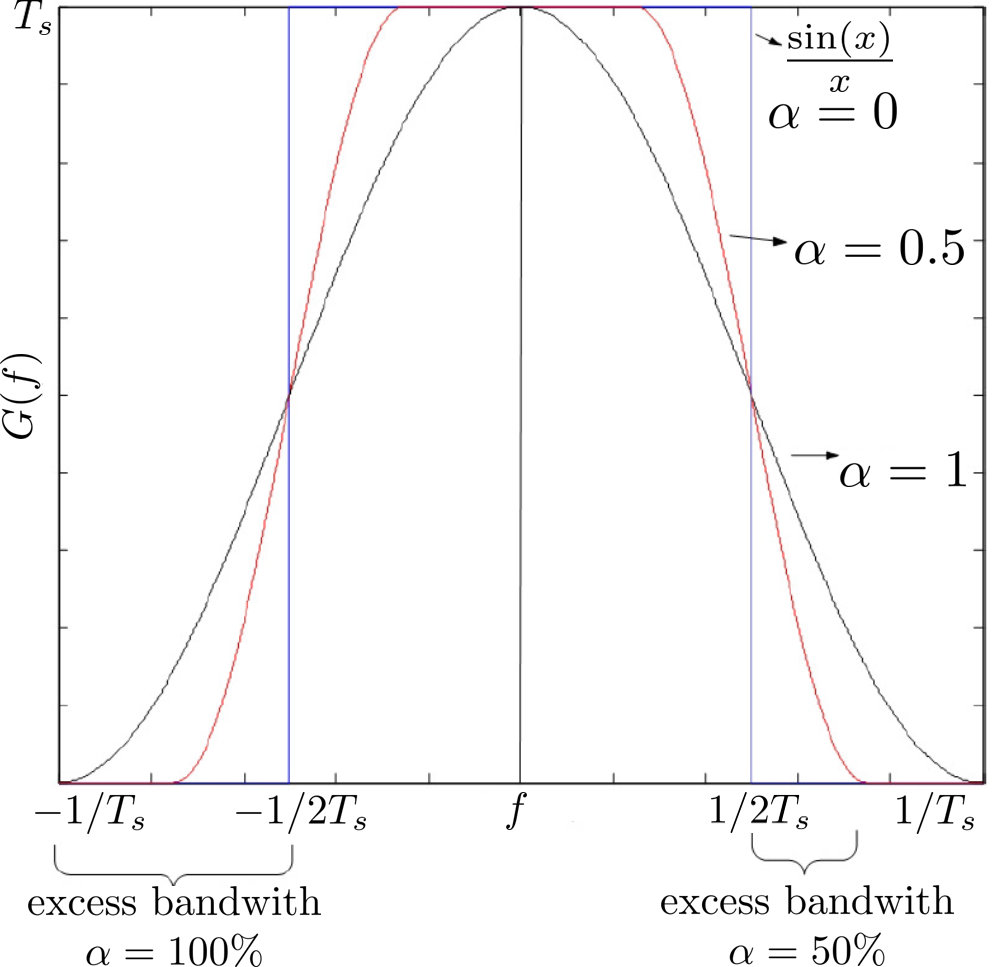
\includegraphics[width=0.35\textwidth]{img/rolloff.png}
\end{figure}

Il est important de se rappeler que c'est la mise en cascade (convolution) de $u(t)$ et $u(-t)$ qui doit être du type Nyquist. Cela signifie que $U(\omega)$ est obtenu par racine carrée de $G(\omega)$.\\
En temporel on a:

\begin{figure}[H]
    \centering
    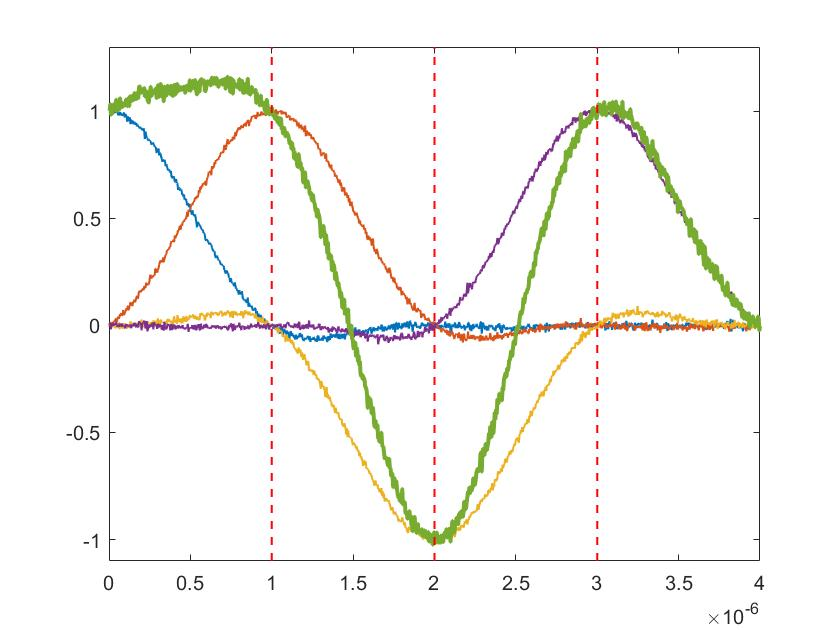
\includegraphics[width=0.6\textwidth]{img/eye.jpg}
\end{figure}

Les instants de passage par zéro sont alignés au $T_b$ seulement parce que le critère de Nyquist est respecté. En sachant que la facteur limitant est le taux $\frac{symb}{sec}$ on pourrait se dire qu'il suffirait d'augmenter au maximum le nombre de $\frac{bit}{symb}$ pour avoir un taux de $\frac{bit}{sec}$ max
\footnote{
$2^{\#bits}=\# symb$
}
. Ceci étant, le rapport SNR reste lui constant et le BER augmentera donc inévitablement si on n'augmente pas la puissance d'émission. Si par contre on ne souhaite pas aumgmenter la puissance tout en gardant un BER constant, la portée du signal s'en retrouve réduite.

\section{Transmission en bande passante}
Nous parlerons ici essentiellement de \textit{modulations linéaires} pour lesquelles le signal modulé peut se mettre sous la forme :
$$ x(t) = \Re{[e_s(t)\ exp(j\omega_ct)]} $$
avec :
$$ e_x(t) = \sum_{n=-\infty}^{\infty} I_n\ u(t-nT) $$
Les $I_n = a_n + j\ b_n = \rho_n\ exp(j\phi_n)$ sont des symboles $\mathbb{C}$ qui appartiennent à un \textit{alphabet} et qui définissent une \textit{constellation}. $u(t)$ est le filtre de mise en forme (en principe en racine de Nyquist).\\
Le fait d'avoir une composante en phase et en quadrature nous permet de faire porter $n_a$ bits sur la composante $a_n$ et $n_b$ sur la composante $b_n$.\\
Si $n_a$ bits en I et $n_b$ bits en Q on a un débit de $(n_a+n_b)/T$ bps, de plus si $n_a = n_b$ on aura une constellation \textbf{Q}uadrature \textbf{A}mplitude \textbf{M}odulation. \\

\begin{figure}[H]
    \centering
    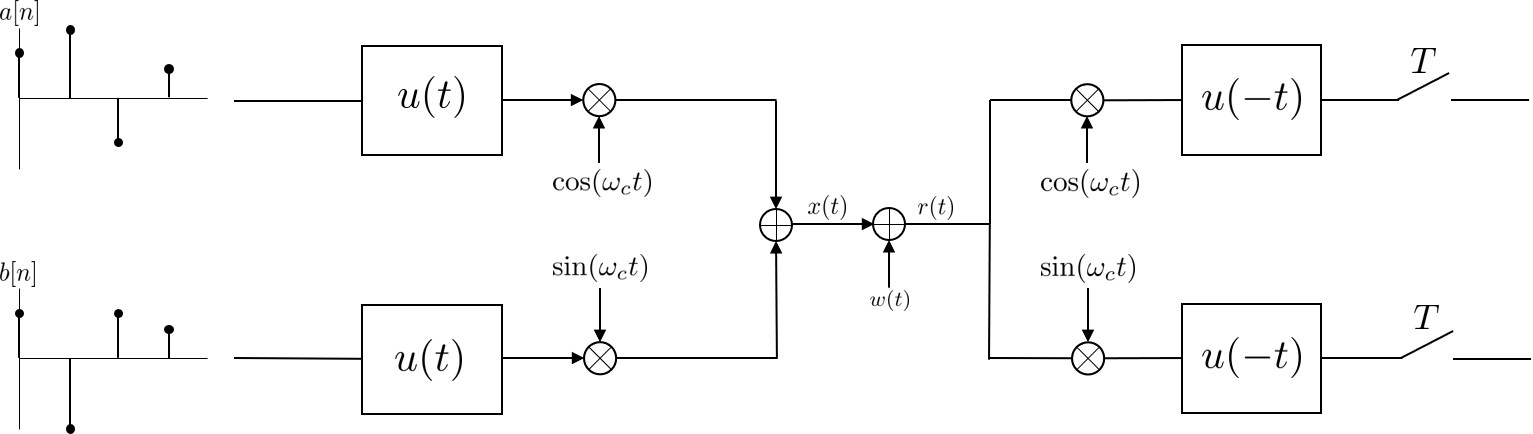
\includegraphics[width=0.9\textwidth]{img/BP.png}
\end{figure}

\begin{align*}
e_x(t) &= \sum_n I_n u(t-nT)\\
x(t) &= \Re{ \left( \sum_n (a[n] + jb[n])\ u(t-nT)\ e^{j\omega_cT} \right) }\\
&=\underbrace{ \sum_n a[n]u[t-nT]}_{x_1}cos(\omega_ct)\ - \ \underbrace{\sum_n b[n] u(t-nT)}_{x_2}sin(\omega_ct)
\end{align*}

Les filtres $u(t)$ servent de filtre passe bas pour ne reprendre que les composantes de Rice ET de filtres adaptés.\\

On peut aussi concevoir des constellations \textbf{P}hase \textbf{S}hift \textbf{K}eying. La première est plus sensible à l'amplitude du vecteur bruit tandis que la dernière est plus sensible à la phase du bruit.
%\samepage{
\begin{multicols}{2}
\noindent
\begin{Figure}
    \centering
    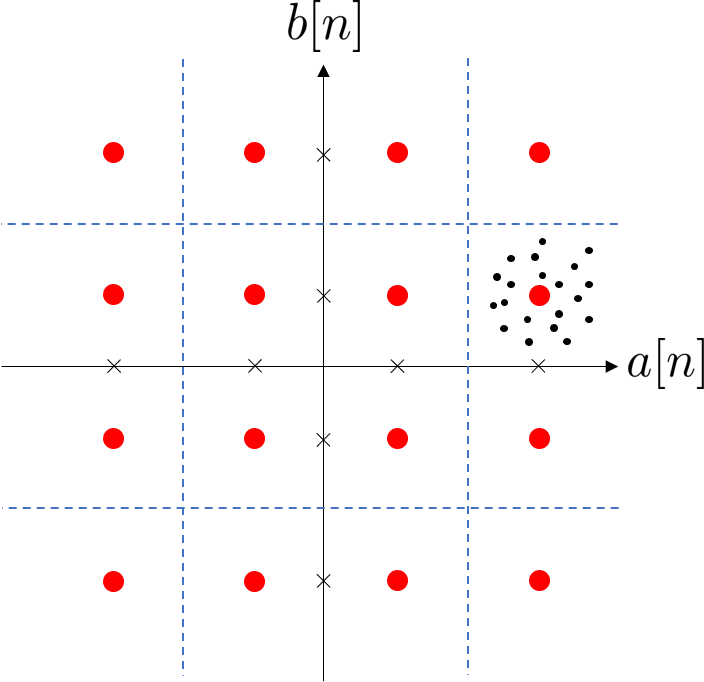
\includegraphics[width=0.7\textwidth]{img/constell2.png}
    \captionof{figure}{QAM-16}
\end{Figure}
\vfill\null
\columnbreak
\noindent
\vspace{2ex}

\begin{Figure}
    \centering
    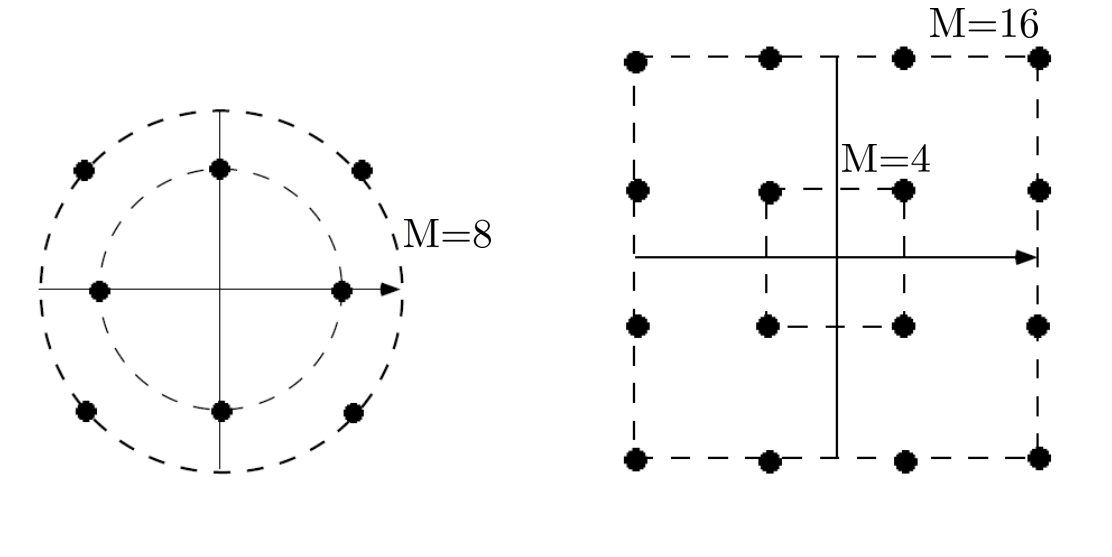
\includegraphics[width=\textwidth]{img/constell.png}
\end{Figure}
\end{multicols}
%}
\subsection{Efficacité spectrale}

La bande occupée par le signal modulé requiert une largeur $B=(1+\alpha)/T_b\ [Hz]$. \\
L'efficacité est calculée comme le débit en bauds sur la largeur de bande consommée: 
$$ \frac{(n_a + n_b)/T_b}{(1+\alpha)/T_b}\ [baud/Hz]$$


\part{Codes correcteurs d'erreur et stratégies de détection}

\section*{Hypothèse}


Les codes classiques ont de meilleurs performance lorsque les erreurs du canal sont indépendantes. Les conditions de transmission peuvent avoir pour répercution de rendre le canal ``à mémoire''. Prenons l'exemple d'un obstacle venant se mettre en travers de l'émetteur et du récepteur durant une période $T_w$. Ceci aura pour effet de confronter des paquets successifs à des taux d'erreur similaires, donnant ainsi une mémoire au canal, ce qui est à éviter. La solution est donc de supprimer cette mémoire en \textit{entrelaçant} les paquets entre eux sur une période $T>T_w$.

\begin{figure}[H]
    \centering
    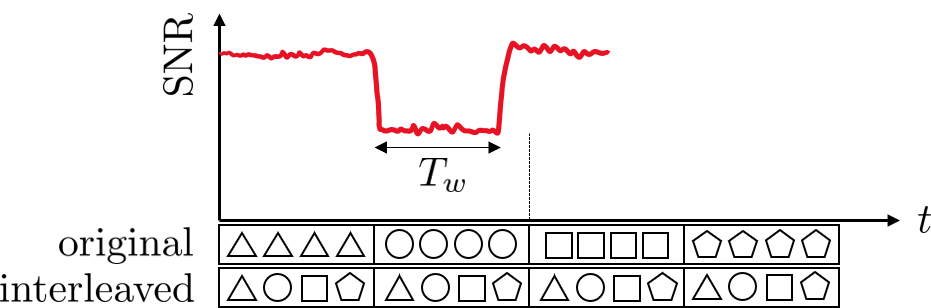
\includegraphics[width=0.5\textwidth]{img/interleaving.png}
    \caption{Processus d'entrelacement}
\end{figure}

\section{Code FEC : Foward error correction}


\subsection{Informations requises}

Les codes correcteurs d'erreur ont besoin de certaines informations à savoir les \textit{probabilités de transition} :
$$ p[y_i | x_j,z_j] $$
\begin{itemize}
\item[•]
$y_i$ la sortie du démodulateur
\item[•]
$x_j$ la sortie du codeur ou de l'entrelaceur
\item[•]
$z_j$ information sur le canal (ici simplement savoir si le brouilleur
\footnote{source d'interférence qui détruis le SNR (voulue ou non) et qui fais passer le $N_0$ à $N_0 + N_j$}
 est actif/inactif)
\end{itemize}

Le fait de choisir un $y_i$ plutôt qu'un autre se fera sur base de décision dont on distingue deux types :
\begin{itemize}
\item
décision dure (hard) : on ne se base que sur le signe du signal reçu.
\item
décision souple (soft) : on se base sur la valeur complète du signal reçu.
\end{itemize}

\subsection{Distance}

La distance en deux mots code est le nombre de bits qui diffèrent d'un mot par rapport à l'autre. Elle est appelée la \textit{distance de Hamming} $d_H$. C'est aussi le poids (la somme des 1 dans un mot code) de la somme des deux signaux, une somme étant équivalente à l'opération XOR. On s'évertuera à minimiser la distance entre le signal reçu et ceux proposés afin de les faire correspondre au mieux. 


\subsection{Concepts de code en blocs linéaires}

On va introduire des bits de redondance à la fin de chaque blocs pour augmenter notre capacité à détecter des erreurs. On pourra aussi dans certains cas les corriger mais pas à chaque fois :

\begin{figure}[H]
    \centering
    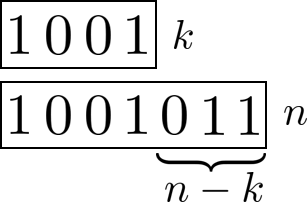
\includegraphics[width=0.15\textwidth]{img/redun.png}
\end{figure}

On a $k$ bits d'entrée, $n$ bits de sortie, un taux de code de $k/n$ et une redondance de $n-k$.\\
Du fait qu'on n'exploite que $2^k$ possibilités des $2^n$, on pourra ensuite détecter si un paquet appartient ou non à ceux définis dans les $2^k$ possibilités et ainsi identifier les erreurs. \\
Exemple :

\begin{multicols}{2}
\begin{Figure}
    \centering
    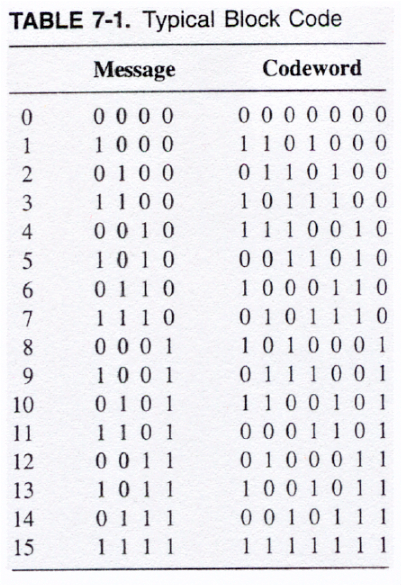
\includegraphics[width=0.7\textwidth]{img/table.png}
\end{Figure}
\vfill\null
\columnbreak
\noindent
$k=4$, $n=7$, $A_3 = 7$, $A_4 = 7$, $A_7=1$ \\\\
Imaginons que 0000 ait été envoyé et que l'on reçoive 0000001. On peux voir que ce dernier mot code n'est pas repris dans la liste de $2^4$ mots possibles, nous sommes donc en mesure de détecter une erreur. De plus on est capables de retrouver le mot d'origine en se ramenant au mot ayant une distance $d_H$ minimale avec celui reçu Soit le mot 0 qui est notre signal envoyé. \\
Si maintenant on avait reçu 0000011, le mot qui s'en rapproche le plus aurait été le 12, qui ne correspond pas à notre mot d'origine. On détecte donc l'erreur mais on ne sait plus la corriger car la distance entre ces deux mots allongés est plus proche de la distance minimale entre tous les mots allongés (ref. $A_3$) que de 0.

\end{multicols}

\subsection{Règle de décodage optimale}

Jusqu'à présent on peut voir la stratégie de minimiser la distance de Hamming comme assez intuitive et coulant de source. Cependant, on peut retomber sur ce même résultat en partant de règles strictes.\\
Nous travaillerons avec des canaux sans mémoire, à symétrie binaire et de probabilité de transition $p$. Pour rappel, la probabilité d'erreur pour une BPSK suit la relation : $p_j = erfc (\sqrt{2E_b/N_{nj}})$

\begin{multicols}{2}
\Large
$p[\mathbf{y}|\mathbf{x}_m,\mathbf{z}] = \prod_{j=1}^n p[y_j|x_{mj},z_j]$
\vfill\null
\columnbreak
\noindent
\begin{Figure}
    \centering
    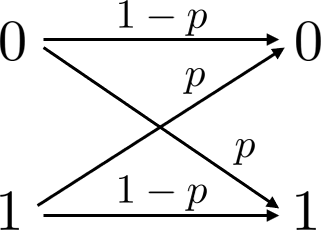
\includegraphics[width=0.3\textwidth]{img/BSC.png}
\end{Figure}
\end{multicols}

Les probabilités de transition se calculent comme suit :

\begin{align*}
p[\mathbf{y}|\mathbf{x}_m,\mathbf{z}] &= \prod_{j \in J} p[y_j|x_{mj}, \overbrace{z_j =1}^{\mathclap{\text{brouilleur inactif}}}] \ \prod_{j \cancel{\in} J} p[y_j|x_{mj},\overbrace{z_j =0}^{\mathclap{\text{brouilleur actif}}}]\\
&= p_1^{d_1} (1-p_1)^{n_1-d_1}\ p_0^{d_0}(1-p_0)^{n-n_1-d_0} \\
\text{Si pas de brouilleur: } &= p^{d_H}(1-p)^{n-d_H} \qquad \text{$p$ une valeur moyenne}
\end{align*}

On va sélectionner le $\mathbf{x}_m$ ayant la plus grande probabilité posteriori $p[\mathbf{x}_m | \mathbf{y}]$. Sachant qu'on ait reçu $\mathbf{y}$, quel est le signal qui a la plus grande probabilité d'avoir été envoyé. Avec Bayes :

$$ p[\mathbf{x}_m | \mathbf{y}] = \dfrac{p[\mathbf{y} | \mathbf{x}_m]\ p[\mathbf{x}_m]}{p[\mathbf{y}]} $$

Le dénominateur étant indépendant du message, on se focalisera sur la maximisation du facteur de gauche du numérateur, le second supposé régulier. On voit donc qu'il suffira de maximiser la probabilité de transition.

\subsubsection*{Décision dure - sans brouilleur}
$$ p[\mathbf{y}|\mathbf{x}_m] = p^{d_H}(1-p)^{n-d_H} $$
On peut maximiser le log cette fonction car le logarithme est une fonction strictement monotone :
$$ ln\ p[\mathbf{y}|\mathbf{x}_m] = d_H\ ln\ p + (n-d_H)ln(1-p) = d_H \ \underbrace{ln\frac{p}{1-p}}_{<0} + \underbrace{n\ln(1-p)}_{cst}$$
On voit donc qu'il faudra minimiser $d_H$ !

\subsubsection*{Décision souple - sans brouilleur}
\begin{align*}
p[y_j|x_j] &= \frac{1}{\sqrt{\pi N_0}}\ \exp\left[- \frac{(y_j - x_j)^2}{N_0}\right]\\
&\downarrow \\
ln\ p[\mathbf{y}|\mathbf{x}_m] &= \sum_{j=1}^n ln\ p[y_j|x_{mj}] \\
&= -\frac{n}{2}\ ln\ p[\pi N_0] - \frac{1}{N_0}\sum_{j=1}^n (y_j-x_j)^2
\end{align*}
Ceci revient à minimiser le terme de droite qui est la distance euclidienne, ce qui revient aussi à maximiser le produit scalaire entre les deux mots codes, ce qui est plutôt intuitif.

\subsubsection*{Décision dure - avec brouilleur}

\begin{align*}
p[\mathbf{y}|\mathbf{x}_m,\mathbf{z}] &= p_1^{d_1} (1-p_1)^{n_1-d_1}\ p_0^{d_0}(1-p_0)^{n-n_1-d_0} \\
&\downarrow \\
ln\ p[\mathbf{y}|\mathbf{x}_m,\mathbf{z}] &= d_1\ ln\frac{p_1}{1-p_1} +\underbrace{ n_1\ ln(1-p_1)}_{cst}\\
&+ \cancel{d_0\ ln\frac{p_0}{1-p_0}} + \underbrace{(n-n_1)\ ln(1-p_0)}_{cst}\\
\intertext{Lorsque le brouilleur est au max, $p_0$ tend vers $1/2$. On ne tiendra donc compte que de la partie où le brouilleur est inactif.}
\end{align*}
Comme $p_1 \leq 0.5$, il est nécessaire de minimiser $d_1$ pour maximiser la probabilité de transition.

\subsubsection*{Décision souple - avec brouilleur}

\begin{align*}
p[y_j|x_j] &= \frac{1}{\sqrt{\pi N_n}}\ \exp\left[- \frac{(y_j - x_j)^2}{N_n}\right]\\
&\downarrow \\
p[\mathbf{y}|\mathbf{x}_m] &= \prod_{j \cancel{\in} J} \frac{1}{\sqrt{\pi N_0}}\ \exp\left[- \frac{(y_j - x_{mj})^2}{N_0}\right] \ +\ \prod_{j \in J} \frac{1}{\sqrt{\pi( N_0+N_j)}}\ \exp\left[- \frac{(y_j - x_{mj})^2}{N_0+N_j}\right] \\
\intertext{avec $\log$}\\
&-\underbrace{\frac{1}{N_0 + N_j}}_{\mathclap{\nearrow \nearrow \ \text{si brouilleur actif}}}\ \sum_{j \in J} (y_j - x_{mj})^2\ -\ \frac{1}{N_0}\sum_{j \cancel{\in} J} (y_j - x_{mj})^2 
\end{align*}
Il faut ici aussi minimiser la distance euclidienne.

\subsection{Comparaison décision souple/dure}

\begin{figure}[H]
    \centering
    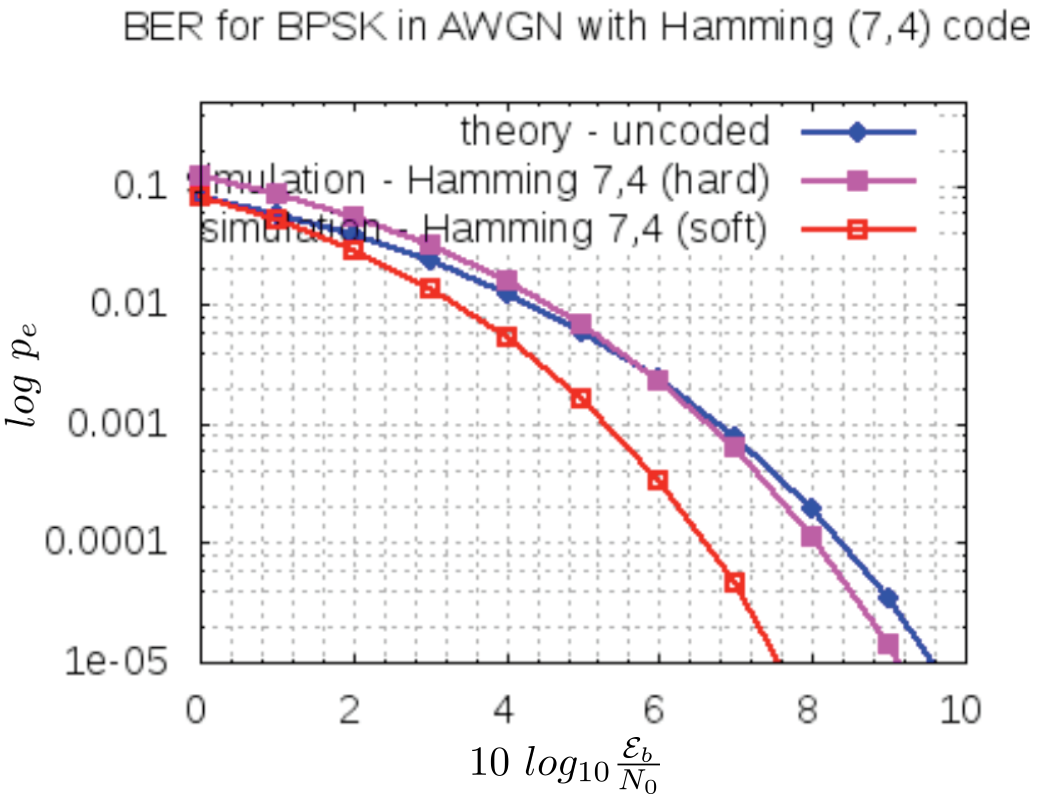
\includegraphics[width=0.7\textwidth]{img/hardsoft.png}
\end{figure}

On peut voir qu'à très mauvais SNR, on se trompe plus de fois si on décide de prendre la distance minimale entre les mots code que si on ne le fait pas. Ceci est dû au fait que l'hypothèse que l'élément envoyé est le plus proche de celui reçu est mauvaise à bas SNR.

\section{Codes convolutifs}

Ce type de code fonctionne en continu à l'opposition de l'utilisation de blocs dans les codes FEC. Souvent utilisé avec des décisions souples, il peut être représenté de différentes manières :

\begin{figure}[H]
    \centering
    \includegraphics[width=0.8\textwidth]{img/state.png}
\end{figure}

On peut faire une analogie entre la variable $D$ et la variable $z$ de la transformée en $z$. $w(D)$ est le train de bits d'entrée. On voit ici que le \textit{taux du code} est de $1/2$ car on a une sortie de 2 bits pour 1 bit d'entrée. Ces deux bits de sortie amènent à 4 états différents possibles. \\
De ce schéma, on peut définir deux représentations du code :

\subsection{Représentation d'état}

\begin{multicols}{2}

\begin{Figure}
    \centering
	 \includegraphics[width=0.7\textwidth]{img/StateRep.png}
\end{Figure}
\vfill\null
\columnbreak
\noindent

L'ordre à suivre est le suivant :\\
Supposons que nous partons de l'état \encircle{00}. On introduit ensuite le bit 1 ce qui nous fait suivre la flèche en tirets. Les deux bits soulignés par celle-ci sont nos bits de sortie pour un 1 en entrée. Enfin, nous atteignons un nouvel état \encircle{10} qui est obtenu en décalant l'état initial dans le temps et en introduisant notre bit d'entrée dans le nouvel état.

\end{multicols}

\subsection{Diagramme en treillis}

Le treillis est une représentation d'état, dépliée au cours du temps: 

\begin{figure}[H]
    \centering
    \includegraphics[width=0.9\textwidth]{img/treillis.png}
\end{figure}

\subsection{Décodage}

Le décodage se fera ici aussi en minimisant les distances de Hamming ou les distance euclidiennes selon que l'on travaille en décisions dures ou souples, entre la séquence reçue et les différentes séquences de la structure. On peut aussi choisir de plutôt que de maximiser la vraisemblance et ainsi minimiser $d_H$, maximiser le $\log$ de la vraisemblance et ainsi tenter de maximiser $\sum_{j=0}^{\infty} ln\ p[y_j|x_{mj}]$. Les $ln\ p[y_j|x_{mj}]$ sont appelées les ``\textit{branch metric}''.\\
L'algorithme de Viterbi nous permet de minimiser le nombre de séquences à comparer avec la séquence reçue en \textit{élaguant} le treillis. La démarche est la suivante : Calculer la $d_H$ de la profondeur 0 à 1 pour toutes les séquences, afficher cette distance au dessus des états candidats et continuer plus en profondeur dans le treillis tout en accumulant les distances. Si deux séquences se rejoignent en un même nœud, on ne garde que celle dont la distance accumulée est la plus faible. On peut ainsi élaguer le treillis en supprimant des séquences :

\begin{figure}[H]
    \centering
    \includegraphics[width=0.7\textwidth]{img/treillisVirb.png}
\end{figure}

On voit ici que les chemins bleu et rouge se rejoignent au même état avec des poids différents. On ne gardera donc que le chemin bleu. \\
On arrivera au final avec une seule séquence valable qui correspondra bien à la séquence envoyée. 

\subsection*{Décision souple}

Si on décide de garder l'information sur la zone dans laquelle l'information a été quantifiée. 

\begin{multicols}{2}

\begin{Figure}
    \centering
	 \includegraphics[width=0.9\textwidth]{img/quant.png}
\end{Figure}
\vfill\null
\columnbreak
\noindent
\begin{Figure}
    \centering
	 \includegraphics[width=0.7\textwidth]{img/quantbis.png}
	 \captionof{figure}{quantification sur 2 bits}
\end{Figure}
\vfill\null
\end{multicols}

Il s'agira alors de maximiser les métriques cumulatives (les chemins avec une $\times$ sont élagués).

\begin{figure}[H]
    \centering
    \includegraphics[width=0.9\textwidth]{img/soft.png}
\end{figure}

\end{document}
